\documentclass[twoside]{book}

% Packages required by doxygen
\usepackage{fixltx2e}
\usepackage{calc}
\usepackage{doxygen}
\usepackage[export]{adjustbox} % also loads graphicx
\usepackage{graphicx}
\usepackage[utf8]{inputenc}
\usepackage{makeidx}
\usepackage{multicol}
\usepackage{multirow}
\PassOptionsToPackage{warn}{textcomp}
\usepackage{textcomp}
\usepackage[nointegrals]{wasysym}
\usepackage[table]{xcolor}

% Font selection
\usepackage[T1]{fontenc}
\usepackage[scaled=.90]{helvet}
\usepackage{courier}
\usepackage{amssymb}
\usepackage{sectsty}
\renewcommand{\familydefault}{\sfdefault}
\allsectionsfont{%
  \fontseries{bc}\selectfont%
  \color{darkgray}%
}
\renewcommand{\DoxyLabelFont}{%
  \fontseries{bc}\selectfont%
  \color{darkgray}%
}
\newcommand{\+}{\discretionary{\mbox{\scriptsize$\hookleftarrow$}}{}{}}

% Page & text layout
\usepackage{geometry}
\geometry{%
  a4paper,%
  top=2.5cm,%
  bottom=2.5cm,%
  left=2.5cm,%
  right=2.5cm%
}
\tolerance=750
\hfuzz=15pt
\hbadness=750
\setlength{\emergencystretch}{15pt}
\setlength{\parindent}{0cm}
\setlength{\parskip}{3ex plus 2ex minus 2ex}
\makeatletter
\renewcommand{\paragraph}{%
  \@startsection{paragraph}{4}{0ex}{-1.0ex}{1.0ex}{%
    \normalfont\normalsize\bfseries\SS@parafont%
  }%
}
\renewcommand{\subparagraph}{%
  \@startsection{subparagraph}{5}{0ex}{-1.0ex}{1.0ex}{%
    \normalfont\normalsize\bfseries\SS@subparafont%
  }%
}
\makeatother

% Headers & footers
\usepackage{fancyhdr}
\pagestyle{fancyplain}
\fancyhead[LE]{\fancyplain{}{\bfseries\thepage}}
\fancyhead[CE]{\fancyplain{}{}}
\fancyhead[RE]{\fancyplain{}{\bfseries\leftmark}}
\fancyhead[LO]{\fancyplain{}{\bfseries\rightmark}}
\fancyhead[CO]{\fancyplain{}{}}
\fancyhead[RO]{\fancyplain{}{\bfseries\thepage}}
\fancyfoot[LE]{\fancyplain{}{}}
\fancyfoot[CE]{\fancyplain{}{}}
\fancyfoot[RE]{\fancyplain{}{\bfseries\scriptsize Generated by Doxygen }}
\fancyfoot[LO]{\fancyplain{}{\bfseries\scriptsize Generated by Doxygen }}
\fancyfoot[CO]{\fancyplain{}{}}
\fancyfoot[RO]{\fancyplain{}{}}
\renewcommand{\footrulewidth}{0.4pt}
\renewcommand{\chaptermark}[1]{%
  \markboth{#1}{}%
}
\renewcommand{\sectionmark}[1]{%
  \markright{\thesection\ #1}%
}

% Indices & bibliography
\usepackage{natbib}
\usepackage[titles]{tocloft}
\setcounter{tocdepth}{3}
\setcounter{secnumdepth}{5}
\makeindex

% Hyperlinks (required, but should be loaded last)
\usepackage{ifpdf}
\ifpdf
  \usepackage[pdftex,pagebackref=true]{hyperref}
\else
  \usepackage[ps2pdf,pagebackref=true]{hyperref}
\fi
\hypersetup{%
  colorlinks=true,%
  linkcolor=blue,%
  citecolor=blue,%
  unicode%
}

% Custom commands
\newcommand{\clearemptydoublepage}{%
  \newpage{\pagestyle{empty}\cleardoublepage}%
}

\usepackage{caption}
\captionsetup{labelsep=space,justification=centering,font={bf},singlelinecheck=off,skip=4pt,position=top}

%===== C O N T E N T S =====

\begin{document}

% Titlepage & ToC
\hypersetup{pageanchor=false,
             bookmarksnumbered=true,
             pdfencoding=unicode
            }
\pagenumbering{alph}
\begin{titlepage}
\vspace*{7cm}
\begin{center}%
{\Large Advanced Algorithms and Parallel Programming Project \\[1ex]\large 1.\+0 }\\
\vspace*{1cm}
{\large Generated by Doxygen 1.8.13}\\
\end{center}
\end{titlepage}
\clearemptydoublepage
\pagenumbering{roman}
\tableofcontents
\clearemptydoublepage
\pagenumbering{arabic}
\hypersetup{pageanchor=true}

%--- Begin generated contents ---
\chapter{A\+A\+P\+P\+\_\+\+Project}
\label{index}\hypertarget{index}{}Advanced Algorithms Project for the course Advanced Algorithms and Parallel Programming

\subsection*{Prerequisites}


\begin{DoxyItemize}
\item Boost Libraries should be installed and should be built with c++11 flag
\item Required libraries for python scripts
\begin{DoxyItemize}
\item pandas
\item numpy
\item matplotlib
\item argparse
\item seaborn
\item contextmanager
\item networkx
\end{DoxyItemize}
\end{DoxyItemize}

\subsection*{How to Build}

After cloning the project execute the commands below in the project folder


\begin{DoxyCode}
cmake .
make
\end{DoxyCode}


\subsection*{How to run}


\begin{DoxyCode}
./out/Project 
\end{DoxyCode}
 \subsection*{How to generate the documentation}

Execute the command below in the project folder


\begin{DoxyCode}
doxygen Doxyfile
\end{DoxyCode}
 
\chapter{Namespace Index}
\section{Namespace List}
Here is a list of all namespaces with brief descriptions\+:\begin{DoxyCompactList}
\item\contentsline{section}{\hyperlink{namespace_utility_structs}{Utility\+Structs} }{\pageref{namespace_utility_structs}}{}
\end{DoxyCompactList}

\chapter{Hierarchical Index}
\section{Class Hierarchy}
This inheritance list is sorted roughly, but not completely, alphabetically\+:\begin{DoxyCompactList}
\item \contentsline{section}{Analyzer}{\pageref{class_analyzer}}{}
\item \contentsline{section}{Application}{\pageref{class_application}}{}
\item \contentsline{section}{Utility\+Structs\+:\+:Edge\+Property}{\pageref{struct_utility_structs_1_1_edge_property}}{}
\item \contentsline{section}{Graph\+Component}{\pageref{class_graph_component}}{}
\begin{DoxyCompactList}
\item \contentsline{section}{Nuutila}{\pageref{class_nuutila}}{}
\item \contentsline{section}{Pearce}{\pageref{class_pearce}}{}
\item \contentsline{section}{Tarjan}{\pageref{class_tarjan}}{}
\end{DoxyCompactList}
\item \contentsline{section}{Session}{\pageref{struct_session}}{}
\item \contentsline{section}{Utility\+Structs\+:\+:Storage\+Items}{\pageref{struct_utility_structs_1_1_storage_items}}{}
\item \contentsline{section}{Utility\+Structs\+:\+:Timer}{\pageref{class_utility_structs_1_1_timer}}{}
\item \contentsline{section}{Utility\+Structs\+:\+:Vertex\+Property}{\pageref{struct_utility_structs_1_1_vertex_property}}{}
\item \contentsline{section}{Visualize}{\pageref{class_visualize}}{}
\end{DoxyCompactList}

\chapter{Class Index}
\section{Class List}
Here are the classes, structs, unions and interfaces with brief descriptions\+:\begin{DoxyCompactList}
\item\contentsline{section}{\hyperlink{class_analyzer}{Analyzer} \\*This class is mainly responsible for the experiment functionality. It also provides the wrapped experiment methods }{\pageref{class_analyzer}}{}
\item\contentsline{section}{\hyperlink{class_application}{Application} \\*This class will contain the main functionalities of the application }{\pageref{class_application}}{}
\item\contentsline{section}{\hyperlink{struct_utility_structs_1_1_edge_property}{Utility\+Structs\+::\+Edge\+Property} \\*This struct contains the edge type info for \hyperlink{class_tarjan}{Tarjan}\textquotesingle{}s S\+CC Algorithm }{\pageref{struct_utility_structs_1_1_edge_property}}{}
\item\contentsline{section}{\hyperlink{class_graph_component}{Graph\+Component} \\*This class is used to read graphs from the file and import them to the Boost Graph objects }{\pageref{class_graph_component}}{}
\item\contentsline{section}{\hyperlink{class_nuutila}{Nuutila} \\*This class contains the implementations of algorithms from the \hyperlink{class_nuutila}{Nuutila}\textquotesingle{}s Paper }{\pageref{class_nuutila}}{}
\item\contentsline{section}{\hyperlink{class_pearce}{Pearce} \\*This class contains the implementation of algorithms from the \hyperlink{class_pearce}{Pearce}\textquotesingle{}s paper }{\pageref{class_pearce}}{}
\item\contentsline{section}{\hyperlink{struct_session}{Session} \\*This struct is used to contain information about the last generated graph directive and the experiment result for users }{\pageref{struct_session}}{}
\item\contentsline{section}{\hyperlink{struct_utility_structs_1_1_storage_items}{Utility\+Structs\+::\+Storage\+Items} \\*This struct is used to store all of the output information of algorithms for later use }{\pageref{struct_utility_structs_1_1_storage_items}}{}
\item\contentsline{section}{\hyperlink{class_tarjan}{Tarjan} \\*This class contains the implementation of algorithms from the \hyperlink{class_tarjan}{Tarjan}\textquotesingle{}s paper }{\pageref{class_tarjan}}{}
\item\contentsline{section}{\hyperlink{class_utility_structs_1_1_timer}{Utility\+Structs\+::\+Timer} \\*This class is used to measure the execution time of a executed function with the same scope }{\pageref{class_utility_structs_1_1_timer}}{}
\item\contentsline{section}{\hyperlink{struct_utility_structs_1_1_vertex_property}{Utility\+Structs\+::\+Vertex\+Property} \\*This struct contains the vertex index info that are used by all of the algorithms }{\pageref{struct_utility_structs_1_1_vertex_property}}{}
\item\contentsline{section}{\hyperlink{class_visualize}{Visualize} \\*This class is used to visualize the information that are gathered from the algorithms }{\pageref{class_visualize}}{}
\end{DoxyCompactList}

\chapter{File Index}
\section{File List}
Here is a list of all files with brief descriptions\+:\begin{DoxyCompactList}
\item\contentsline{section}{header/\hyperlink{analyzer_8h}{analyzer.\+h} }{\pageref{analyzer_8h}}{}
\item\contentsline{section}{header/\hyperlink{application_8h}{application.\+h} }{\pageref{application_8h}}{}
\item\contentsline{section}{header/\hyperlink{graphcomponent_8h}{graphcomponent.\+h} }{\pageref{graphcomponent_8h}}{}
\item\contentsline{section}{header/\hyperlink{nuutila_8h}{nuutila.\+h} }{\pageref{nuutila_8h}}{}
\item\contentsline{section}{header/\hyperlink{pearce_8h}{pearce.\+h} }{\pageref{pearce_8h}}{}
\item\contentsline{section}{header/\hyperlink{tarjan_8h}{tarjan.\+h} }{\pageref{tarjan_8h}}{}
\item\contentsline{section}{header/\hyperlink{utilities_8h}{utilities.\+h} }{\pageref{utilities_8h}}{}
\item\contentsline{section}{header/\hyperlink{visualize_8h}{visualize.\+h} }{\pageref{visualize_8h}}{}
\item\contentsline{section}{src/\hyperlink{analysis_8py}{analysis.\+py} }{\pageref{analysis_8py}}{}
\item\contentsline{section}{src/\hyperlink{analyzer_8cpp}{analyzer.\+cpp} }{\pageref{analyzer_8cpp}}{}
\item\contentsline{section}{src/\hyperlink{application_8cpp}{application.\+cpp} }{\pageref{application_8cpp}}{}
\item\contentsline{section}{src/\hyperlink{generate__graph__directories_8py}{generate\+\_\+graph\+\_\+directories.\+py} }{\pageref{generate__graph__directories_8py}}{}
\item\contentsline{section}{src/\hyperlink{graphcomponent_8cpp}{graphcomponent.\+cpp} }{\pageref{graphcomponent_8cpp}}{}
\item\contentsline{section}{src/\hyperlink{main_8cpp}{main.\+cpp} }{\pageref{main_8cpp}}{}
\item\contentsline{section}{src/\hyperlink{nuutila_8cpp}{nuutila.\+cpp} }{\pageref{nuutila_8cpp}}{}
\item\contentsline{section}{src/\hyperlink{pearce_8cpp}{pearce.\+cpp} }{\pageref{pearce_8cpp}}{}
\item\contentsline{section}{src/\hyperlink{tarjan_8cpp}{tarjan.\+cpp} }{\pageref{tarjan_8cpp}}{}
\item\contentsline{section}{src/\hyperlink{visualize_8cpp}{visualize.\+cpp} }{\pageref{visualize_8cpp}}{}
\end{DoxyCompactList}

\chapter{Namespace Documentation}
\hypertarget{namespace_utility_structs}{}\section{Utility\+Structs Namespace Reference}
\label{namespace_utility_structs}\index{Utility\+Structs@{Utility\+Structs}}
\subsection*{Classes}
\begin{DoxyCompactItemize}
\item 
struct \hyperlink{struct_utility_structs_1_1_edge_property}{Edge\+Property}
\begin{DoxyCompactList}\small\item\em This struct contains the edge type info for \hyperlink{class_tarjan}{Tarjan}\textquotesingle{}s S\+CC Algorithm. \end{DoxyCompactList}\item 
struct \hyperlink{struct_utility_structs_1_1_storage_items}{Storage\+Items}
\begin{DoxyCompactList}\small\item\em This struct is used to store all of the output information of algorithms for later use. \end{DoxyCompactList}\item 
class \hyperlink{class_utility_structs_1_1_timer}{Timer}
\begin{DoxyCompactList}\small\item\em This class is used to measure the execution time of a executed function with the same scope. \end{DoxyCompactList}\item 
struct \hyperlink{struct_utility_structs_1_1_vertex_property}{Vertex\+Property}
\begin{DoxyCompactList}\small\item\em This struct contains the vertex index info that are used by all of the algorithms. \end{DoxyCompactList}\end{DoxyCompactItemize}

\chapter{Class Documentation}
\hypertarget{class_analyzer}{}\section{Analyzer Class Reference}
\label{class_analyzer}\index{Analyzer@{Analyzer}}


{\ttfamily \#include $<$analyzer.\+h$>$}

\subsection*{Public Member Functions}
\begin{DoxyCompactItemize}
\item 
\hyperlink{class_analyzer_a1be2ff17bba265bdef6e1b44748eaf96_a1be2ff17bba265bdef6e1b44748eaf96}{Analyzer} ()
\item 
\hyperlink{class_analyzer_a2aed8194a48a8385ef271af3bd6fdd42_a2aed8194a48a8385ef271af3bd6fdd42}{Analyzer} (std\+::string \&dirname)
\item 
std\+::vector$<$ std\+::string $>$ \hyperlink{class_analyzer_a7903ffdba689848dd199139e5dacf1bc_a7903ffdba689848dd199139e5dacf1bc}{get\+Input\+List} (std\+::string \&dir\+Path)
\item 
std\+::string \hyperlink{class_analyzer_a9108681fee1078aed1af2ddee58cc55c_a9108681fee1078aed1af2ddee58cc55c}{current\+Date\+Time} ()
\item 
void \hyperlink{class_analyzer_a471ed64111b58f49cfee911b5db93ada_a471ed64111b58f49cfee911b5db93ada}{solve\+\_\+with\+\_\+all} (std\+::string \&input\+File)
\item 
void \hyperlink{class_analyzer_a8207cd71986d26dc8abda1a807490ab2_a8207cd71986d26dc8abda1a807490ab2}{solve\+\_\+with\+\_\+tarjan} (std\+::string \&input\+File)
\item 
void \hyperlink{class_analyzer_a5ac77dbb2bbea6b34af561272705d64e_a5ac77dbb2bbea6b34af561272705d64e}{solve\+\_\+with\+\_\+nuutila} (std\+::string \&input\+File)
\item 
void \hyperlink{class_analyzer_a6009c58addbb9730b54580a5f01ddce7_a6009c58addbb9730b54580a5f01ddce7}{solve\+\_\+with\+\_\+pearce} (std\+::string \&input\+File)
\item 
std\+::string \hyperlink{class_analyzer_ae4637e33a985efefebf2a10502be351c_ae4637e33a985efefebf2a10502be351c}{benchmark\+\_\+comparison} (bool write\+\_\+to\+\_\+file, bool is\+Csv, std\+::string \&input\+Directory)
\end{DoxyCompactItemize}
\subsection*{Public Attributes}
\begin{DoxyCompactItemize}
\item 
std\+::vector$<$ std\+::string $>$ \hyperlink{class_analyzer_a567b5d8b2bbdde28b489834c1644446e_a567b5d8b2bbdde28b489834c1644446e}{graph\+List}
\item 
\hyperlink{class_visualize}{Visualize} \hyperlink{class_analyzer_ae32079d0816589617a0c76b1d4cf881b_ae32079d0816589617a0c76b1d4cf881b}{v}
\end{DoxyCompactItemize}


\subsection{Detailed Description}
This class will test the algorithms with different settings to create a basis for analysis and a comparison baseline 

\subsection{Constructor \& Destructor Documentation}
\mbox{\Hypertarget{class_analyzer_a1be2ff17bba265bdef6e1b44748eaf96_a1be2ff17bba265bdef6e1b44748eaf96}\label{class_analyzer_a1be2ff17bba265bdef6e1b44748eaf96_a1be2ff17bba265bdef6e1b44748eaf96}} 
\index{Analyzer@{Analyzer}!Analyzer@{Analyzer}}
\index{Analyzer@{Analyzer}!Analyzer@{Analyzer}}
\subsubsection{\texorpdfstring{Analyzer()}{Analyzer()}\hspace{0.1cm}{\footnotesize\ttfamily [1/2]}}
{\footnotesize\ttfamily Analyzer\+::\+Analyzer (\begin{DoxyParamCaption}{ }\end{DoxyParamCaption})\hspace{0.3cm}{\ttfamily [inline]}}

\mbox{\Hypertarget{class_analyzer_a2aed8194a48a8385ef271af3bd6fdd42_a2aed8194a48a8385ef271af3bd6fdd42}\label{class_analyzer_a2aed8194a48a8385ef271af3bd6fdd42_a2aed8194a48a8385ef271af3bd6fdd42}} 
\index{Analyzer@{Analyzer}!Analyzer@{Analyzer}}
\index{Analyzer@{Analyzer}!Analyzer@{Analyzer}}
\subsubsection{\texorpdfstring{Analyzer()}{Analyzer()}\hspace{0.1cm}{\footnotesize\ttfamily [2/2]}}
{\footnotesize\ttfamily Analyzer\+::\+Analyzer (\begin{DoxyParamCaption}\item[{std\+::string \&}]{dirname }\end{DoxyParamCaption})\hspace{0.3cm}{\ttfamily [inline]}}



\subsection{Member Function Documentation}
\mbox{\Hypertarget{class_analyzer_ae4637e33a985efefebf2a10502be351c_ae4637e33a985efefebf2a10502be351c}\label{class_analyzer_ae4637e33a985efefebf2a10502be351c_ae4637e33a985efefebf2a10502be351c}} 
\index{Analyzer@{Analyzer}!benchmark\+\_\+comparison@{benchmark\+\_\+comparison}}
\index{benchmark\+\_\+comparison@{benchmark\+\_\+comparison}!Analyzer@{Analyzer}}
\subsubsection{\texorpdfstring{benchmark\+\_\+comparison()}{benchmark\_comparison()}}
{\footnotesize\ttfamily std\+::string Analyzer\+::benchmark\+\_\+comparison (\begin{DoxyParamCaption}\item[{bool}]{write\+\_\+to\+\_\+file,  }\item[{bool}]{is\+Csv,  }\item[{std\+::string \&}]{input\+Directory }\end{DoxyParamCaption})}

\mbox{\Hypertarget{class_analyzer_a9108681fee1078aed1af2ddee58cc55c_a9108681fee1078aed1af2ddee58cc55c}\label{class_analyzer_a9108681fee1078aed1af2ddee58cc55c_a9108681fee1078aed1af2ddee58cc55c}} 
\index{Analyzer@{Analyzer}!current\+Date\+Time@{current\+Date\+Time}}
\index{current\+Date\+Time@{current\+Date\+Time}!Analyzer@{Analyzer}}
\subsubsection{\texorpdfstring{current\+Date\+Time()}{currentDateTime()}}
{\footnotesize\ttfamily std\+::string Analyzer\+::current\+Date\+Time (\begin{DoxyParamCaption}{ }\end{DoxyParamCaption})}

\mbox{\Hypertarget{class_analyzer_a7903ffdba689848dd199139e5dacf1bc_a7903ffdba689848dd199139e5dacf1bc}\label{class_analyzer_a7903ffdba689848dd199139e5dacf1bc_a7903ffdba689848dd199139e5dacf1bc}} 
\index{Analyzer@{Analyzer}!get\+Input\+List@{get\+Input\+List}}
\index{get\+Input\+List@{get\+Input\+List}!Analyzer@{Analyzer}}
\subsubsection{\texorpdfstring{get\+Input\+List()}{getInputList()}}
{\footnotesize\ttfamily std\+::vector$<$ std\+::string $>$ Analyzer\+::get\+Input\+List (\begin{DoxyParamCaption}\item[{std\+::string \&}]{dir\+Path }\end{DoxyParamCaption})}

\mbox{\Hypertarget{class_analyzer_a471ed64111b58f49cfee911b5db93ada_a471ed64111b58f49cfee911b5db93ada}\label{class_analyzer_a471ed64111b58f49cfee911b5db93ada_a471ed64111b58f49cfee911b5db93ada}} 
\index{Analyzer@{Analyzer}!solve\+\_\+with\+\_\+all@{solve\+\_\+with\+\_\+all}}
\index{solve\+\_\+with\+\_\+all@{solve\+\_\+with\+\_\+all}!Analyzer@{Analyzer}}
\subsubsection{\texorpdfstring{solve\+\_\+with\+\_\+all()}{solve\_with\_all()}}
{\footnotesize\ttfamily void Analyzer\+::solve\+\_\+with\+\_\+all (\begin{DoxyParamCaption}\item[{std\+::string \&}]{input\+File }\end{DoxyParamCaption})}

\mbox{\Hypertarget{class_analyzer_a5ac77dbb2bbea6b34af561272705d64e_a5ac77dbb2bbea6b34af561272705d64e}\label{class_analyzer_a5ac77dbb2bbea6b34af561272705d64e_a5ac77dbb2bbea6b34af561272705d64e}} 
\index{Analyzer@{Analyzer}!solve\+\_\+with\+\_\+nuutila@{solve\+\_\+with\+\_\+nuutila}}
\index{solve\+\_\+with\+\_\+nuutila@{solve\+\_\+with\+\_\+nuutila}!Analyzer@{Analyzer}}
\subsubsection{\texorpdfstring{solve\+\_\+with\+\_\+nuutila()}{solve\_with\_nuutila()}}
{\footnotesize\ttfamily void Analyzer\+::solve\+\_\+with\+\_\+nuutila (\begin{DoxyParamCaption}\item[{std\+::string \&}]{input\+File }\end{DoxyParamCaption})}

\mbox{\Hypertarget{class_analyzer_a6009c58addbb9730b54580a5f01ddce7_a6009c58addbb9730b54580a5f01ddce7}\label{class_analyzer_a6009c58addbb9730b54580a5f01ddce7_a6009c58addbb9730b54580a5f01ddce7}} 
\index{Analyzer@{Analyzer}!solve\+\_\+with\+\_\+pearce@{solve\+\_\+with\+\_\+pearce}}
\index{solve\+\_\+with\+\_\+pearce@{solve\+\_\+with\+\_\+pearce}!Analyzer@{Analyzer}}
\subsubsection{\texorpdfstring{solve\+\_\+with\+\_\+pearce()}{solve\_with\_pearce()}}
{\footnotesize\ttfamily void Analyzer\+::solve\+\_\+with\+\_\+pearce (\begin{DoxyParamCaption}\item[{std\+::string \&}]{input\+File }\end{DoxyParamCaption})}

\mbox{\Hypertarget{class_analyzer_a8207cd71986d26dc8abda1a807490ab2_a8207cd71986d26dc8abda1a807490ab2}\label{class_analyzer_a8207cd71986d26dc8abda1a807490ab2_a8207cd71986d26dc8abda1a807490ab2}} 
\index{Analyzer@{Analyzer}!solve\+\_\+with\+\_\+tarjan@{solve\+\_\+with\+\_\+tarjan}}
\index{solve\+\_\+with\+\_\+tarjan@{solve\+\_\+with\+\_\+tarjan}!Analyzer@{Analyzer}}
\subsubsection{\texorpdfstring{solve\+\_\+with\+\_\+tarjan()}{solve\_with\_tarjan()}}
{\footnotesize\ttfamily void Analyzer\+::solve\+\_\+with\+\_\+tarjan (\begin{DoxyParamCaption}\item[{std\+::string \&}]{input\+File }\end{DoxyParamCaption})}



\subsection{Member Data Documentation}
\mbox{\Hypertarget{class_analyzer_a567b5d8b2bbdde28b489834c1644446e_a567b5d8b2bbdde28b489834c1644446e}\label{class_analyzer_a567b5d8b2bbdde28b489834c1644446e_a567b5d8b2bbdde28b489834c1644446e}} 
\index{Analyzer@{Analyzer}!graph\+List@{graph\+List}}
\index{graph\+List@{graph\+List}!Analyzer@{Analyzer}}
\subsubsection{\texorpdfstring{graph\+List}{graphList}}
{\footnotesize\ttfamily std\+::vector$<$std\+::string$>$ Analyzer\+::graph\+List}

\mbox{\Hypertarget{class_analyzer_ae32079d0816589617a0c76b1d4cf881b_ae32079d0816589617a0c76b1d4cf881b}\label{class_analyzer_ae32079d0816589617a0c76b1d4cf881b_ae32079d0816589617a0c76b1d4cf881b}} 
\index{Analyzer@{Analyzer}!v@{v}}
\index{v@{v}!Analyzer@{Analyzer}}
\subsubsection{\texorpdfstring{v}{v}}
{\footnotesize\ttfamily \hyperlink{class_visualize}{Visualize} Analyzer\+::v}



The documentation for this class was generated from the following files\+:\begin{DoxyCompactItemize}
\item 
header/\hyperlink{analyzer_8h}{analyzer.\+h}\item 
src/\hyperlink{analyzer_8cpp}{analyzer.\+cpp}\end{DoxyCompactItemize}

\hypertarget{class_application}{}\section{Application Class Reference}
\label{class_application}\index{Application@{Application}}


This class will contain the main functionalities of the application.  




{\ttfamily \#include $<$application.\+h$>$}

\subsection*{Public Member Functions}
\begin{DoxyCompactItemize}
\item 
\hyperlink{class_application_afa8cc05ce6b6092be5ecdfdae44e05f8}{Application} ()
\item 
void \hyperlink{class_application_adecc88549e44815bd94985ea043b733f}{run} (\hyperlink{struct_session}{Session} \&s)
\item 
void \hyperlink{class_application_abf73a60a6a2e4b83a675de777273d12c}{welcome\+Screen} (\hyperlink{struct_session}{Session} \&s)
\item 
std\+::string \hyperlink{class_application_a169c37596e9a7a9e0546700876adcbe7}{generate\+Graph} (\hyperlink{struct_session}{Session} \&s)
\item 
std\+::string \hyperlink{class_application_a1d9cfbea705655427e7d1847de2567c1}{run\+Experiment} (\hyperlink{struct_session}{Session} \&s)
\item 
void \hyperlink{class_application_adb639e3593f8f6f4dcb3d89d690eb538}{run\+Debug\+Mode} (\hyperlink{struct_session}{Session} \&s)
\item 
void \hyperlink{class_application_ae0d3919fe03bae0b3ce31ef4be49374d}{analyze\+Experiment} (\hyperlink{struct_session}{Session} \&s)
\end{DoxyCompactItemize}
\subsection*{Public Attributes}
\begin{DoxyCompactItemize}
\item 
\hyperlink{class_visualize}{Visualize} \hyperlink{class_application_a96cff2295a95d7e6de06638bb7e61243}{v}
\end{DoxyCompactItemize}


\subsection{Detailed Description}
This class will contain the main functionalities of the application. 

This class acts as a wrapper for the whole application. Every functionality is shown to user via parameter updates, menus and choices. 

Definition at line 15 of file application.\+h.



\subsection{Constructor \& Destructor Documentation}
\mbox{\Hypertarget{class_application_afa8cc05ce6b6092be5ecdfdae44e05f8}\label{class_application_afa8cc05ce6b6092be5ecdfdae44e05f8}} 
\index{Application@{Application}!Application@{Application}}
\index{Application@{Application}!Application@{Application}}
\subsubsection{\texorpdfstring{Application()}{Application()}}
{\footnotesize\ttfamily Application\+::\+Application (\begin{DoxyParamCaption}{ }\end{DoxyParamCaption})\hspace{0.3cm}{\ttfamily [inline]}}



Definition at line 18 of file application.\+h.


\begin{DoxyCode}
18                  \{
19     \};
\end{DoxyCode}


\subsection{Member Function Documentation}
\mbox{\Hypertarget{class_application_ae0d3919fe03bae0b3ce31ef4be49374d}\label{class_application_ae0d3919fe03bae0b3ce31ef4be49374d}} 
\index{Application@{Application}!analyze\+Experiment@{analyze\+Experiment}}
\index{analyze\+Experiment@{analyze\+Experiment}!Application@{Application}}
\subsubsection{\texorpdfstring{analyze\+Experiment()}{analyzeExperiment()}}
{\footnotesize\ttfamily void Application\+::analyze\+Experiment (\begin{DoxyParamCaption}\item[{\hyperlink{struct_session}{Session} \&}]{s }\end{DoxyParamCaption})}



Definition at line 73 of file application.\+cpp.


\begin{DoxyCode}
73                                              \{
74     \hyperlink{class_application_a96cff2295a95d7e6de06638bb7e61243}{v}.\hyperlink{class_visualize_a29f27ff8c5e59163eea2be42ff372405}{printProgramEntry}(s);
75     \hyperlink{class_application_a96cff2295a95d7e6de06638bb7e61243}{v}.\hyperlink{class_visualize_abce6cd538dc0715b21851e0bf0377d85}{printLine}(\textcolor{stringliteral}{""});
76     std::string Program = \textcolor{stringliteral}{"python src/python/analysis.py"};
77     std::string filename = s.\hyperlink{struct_session_a256b14530b834d61ce85bab451694b8c}{csv};
78     \textcolor{keywordtype}{char} choice ;
79     \textcolor{keywordflow}{if}(filename == \textcolor{stringliteral}{"None"})\{
80         \hyperlink{class_application_a96cff2295a95d7e6de06638bb7e61243}{v}.\hyperlink{class_visualize_abce6cd538dc0715b21851e0bf0377d85}{printLine}(\textcolor{stringliteral}{"Please enter the name of the experiment csv file:"});
81         \hyperlink{class_application_a96cff2295a95d7e6de06638bb7e61243}{v}.\hyperlink{class_visualize_ac0be9ece2d80a7d1e34724fb87424216}{printProgramBottom}();
82         std::cout << \textcolor{stringliteral}{"|>> "};
83         std::cin >> filename;
84     \}\textcolor{keywordflow}{else}\{
85         \hyperlink{class_application_a96cff2295a95d7e6de06638bb7e61243}{v}.\hyperlink{class_visualize_abce6cd538dc0715b21851e0bf0377d85}{printLine}(\textcolor{stringliteral}{"Do you want to provide a different csv file ? (y/n)"});
86         \hyperlink{class_application_a96cff2295a95d7e6de06638bb7e61243}{v}.\hyperlink{class_visualize_ac0be9ece2d80a7d1e34724fb87424216}{printProgramBottom}();
87         std::cout << \textcolor{stringliteral}{"|>>"};
88         std::cin >> choice;
89         \textcolor{keywordflow}{switch}(choice)\{
90             \textcolor{keywordflow}{case} \textcolor{charliteral}{'y'}:
91                 \hyperlink{class_application_a96cff2295a95d7e6de06638bb7e61243}{v}.\hyperlink{class_visualize_a29f27ff8c5e59163eea2be42ff372405}{printProgramEntry}(s);
92                 \hyperlink{class_application_a96cff2295a95d7e6de06638bb7e61243}{v}.\hyperlink{class_visualize_abce6cd538dc0715b21851e0bf0377d85}{printLine}(\textcolor{stringliteral}{""});
93                 \hyperlink{class_application_a96cff2295a95d7e6de06638bb7e61243}{v}.\hyperlink{class_visualize_abce6cd538dc0715b21851e0bf0377d85}{printLine}(\textcolor{stringliteral}{"Please enter the name of the experiment csv file:"});
94                 \hyperlink{class_application_a96cff2295a95d7e6de06638bb7e61243}{v}.\hyperlink{class_visualize_ac0be9ece2d80a7d1e34724fb87424216}{printProgramBottom}();
95                 std::cout << \textcolor{stringliteral}{"|>> "};
96                 std::cin >> filename;
97                 \textcolor{keywordflow}{break};
98             \textcolor{keywordflow}{case} \textcolor{charliteral}{'n'}:
99                 \textcolor{keywordflow}{break};
100         \}
101 
102     \}
103     Program += (\textcolor{stringliteral}{" "} + filename);
104     std::system(Program.c\_str());
105     \hyperlink{class_application_a96cff2295a95d7e6de06638bb7e61243}{v}.\hyperlink{class_visualize_abce6cd538dc0715b21851e0bf0377d85}{printLine}(\textcolor{stringliteral}{"Press c to Continue, q to quit"});
106         std::cout << \textcolor{stringliteral}{"|>> "};
107         std::string branch;
108         std::cin >> branch;
109         \textcolor{keywordflow}{if}(branch == \textcolor{stringliteral}{"c"})\{
110             \hyperlink{class_application_a96cff2295a95d7e6de06638bb7e61243}{v}.\hyperlink{class_visualize_a29f27ff8c5e59163eea2be42ff372405}{printProgramEntry}(s);
111             \hyperlink{class_application_abf73a60a6a2e4b83a675de777273d12c}{welcomeScreen}(s);
112         \}\textcolor{keywordflow}{else} \textcolor{keywordflow}{if} (branch == \textcolor{stringliteral}{"q"})\{
113             \textcolor{keywordflow}{return};
114         \}
115 \}
\end{DoxyCode}
\mbox{\Hypertarget{class_application_a169c37596e9a7a9e0546700876adcbe7}\label{class_application_a169c37596e9a7a9e0546700876adcbe7}} 
\index{Application@{Application}!generate\+Graph@{generate\+Graph}}
\index{generate\+Graph@{generate\+Graph}!Application@{Application}}
\subsubsection{\texorpdfstring{generate\+Graph()}{generateGraph()}}
{\footnotesize\ttfamily std\+::string Application\+::generate\+Graph (\begin{DoxyParamCaption}\item[{\hyperlink{struct_session}{Session} \&}]{s }\end{DoxyParamCaption})}



Definition at line 120 of file application.\+cpp.


\begin{DoxyCode}
121 \{
122     
123     \hyperlink{class_application_a96cff2295a95d7e6de06638bb7e61243}{v}.\hyperlink{class_visualize_a29f27ff8c5e59163eea2be42ff372405}{printProgramEntry}(s);
124     \hyperlink{class_application_a96cff2295a95d7e6de06638bb7e61243}{v}.\hyperlink{class_visualize_abce6cd538dc0715b21851e0bf0377d85}{printLine}(\textcolor{stringliteral}{""});
125     std::string Program = \textcolor{stringliteral}{"python src/python/generate\_graph\_directories.py"};
126     std::string dir\_name;
127     std::string numOfGraph;
128     std::string single\_class;
129     \textcolor{keywordtype}{int} singleC = 0;
130     \hyperlink{class_application_a96cff2295a95d7e6de06638bb7e61243}{v}.\hyperlink{class_visualize_abce6cd538dc0715b21851e0bf0377d85}{printLine}(\textcolor{stringliteral}{"Please enter the name of the output folder:"});
131     std::cout << \textcolor{stringliteral}{"|>> "};
132     std::cin >> dir\_name;
133     s.\hyperlink{struct_session_aecaa42a56f197e0874041533ccb358a6}{graph\_dir} = dir\_name;
134     \hyperlink{class_application_a96cff2295a95d7e6de06638bb7e61243}{v}.\hyperlink{class_visualize_abce6cd538dc0715b21851e0bf0377d85}{printLine}(\textcolor{stringliteral}{"Please enter the number of graph instances for each node class:"});
135     std::cout << \textcolor{stringliteral}{"|>> "};
136     std::cin >> numOfGraph;
137     \hyperlink{class_application_a96cff2295a95d7e6de06638bb7e61243}{v}.\hyperlink{class_visualize_abce6cd538dc0715b21851e0bf0377d85}{printLine}(\textcolor{stringliteral}{"Would you like to choose the node classes specifically ?:( y or n )"});
138     std::cout << \textcolor{stringliteral}{"|>> "};
139     std::cin >> single\_class;
140     \textcolor{keywordflow}{if}(single\_class == \textcolor{stringliteral}{"n"})
141     \{   
142         \hyperlink{class_application_a96cff2295a95d7e6de06638bb7e61243}{v}.\hyperlink{class_visualize_abce6cd538dc0715b21851e0bf0377d85}{printLine}(\textcolor{stringliteral}{"The output folder is: "} + dir\_name);
143         \hyperlink{class_application_a96cff2295a95d7e6de06638bb7e61243}{v}.\hyperlink{class_visualize_abce6cd538dc0715b21851e0bf0377d85}{printLine}(\textcolor{stringliteral}{"The number of graphs per each class is "} + numOfGraph);
144         std::string command;
145         command = Program + \textcolor{stringliteral}{" "} + numOfGraph + \textcolor{stringliteral}{" "} + dir\_name;
146         std::system(command.c\_str());
147          \hyperlink{class_application_a96cff2295a95d7e6de06638bb7e61243}{v}.\hyperlink{class_visualize_abce6cd538dc0715b21851e0bf0377d85}{printLine}(\textcolor{stringliteral}{"Press c to Continue, q to quit"});
148         std::cout << \textcolor{stringliteral}{"|>> "};
149         std::string branch;
150         std::cin >> branch;
151         \textcolor{keywordflow}{if}(branch == \textcolor{stringliteral}{"c"})\{
152             \hyperlink{class_application_a96cff2295a95d7e6de06638bb7e61243}{v}.\hyperlink{class_visualize_a29f27ff8c5e59163eea2be42ff372405}{printProgramEntry}(s);
153             \hyperlink{class_application_abf73a60a6a2e4b83a675de777273d12c}{welcomeScreen}(s);
154         \}\textcolor{keywordflow}{else} \textcolor{keywordflow}{if} (branch == \textcolor{stringliteral}{"q"})\{
155             \textcolor{keywordflow}{return} dir\_name;
156         \}
157     \}\textcolor{keywordflow}{else}\{
158         \hyperlink{class_application_a96cff2295a95d7e6de06638bb7e61243}{v}.\hyperlink{class_visualize_a29f27ff8c5e59163eea2be42ff372405}{printProgramEntry}(s);
159         \hyperlink{class_application_a96cff2295a95d7e6de06638bb7e61243}{v}.\hyperlink{class_visualize_abce6cd538dc0715b21851e0bf0377d85}{printLine}(\textcolor{stringliteral}{""});
160         \hyperlink{class_application_a96cff2295a95d7e6de06638bb7e61243}{v}.\hyperlink{class_visualize_abce6cd538dc0715b21851e0bf0377d85}{printLine}(\textcolor{stringliteral}{"The Graph Classes are below:"});
161         \hyperlink{class_application_a96cff2295a95d7e6de06638bb7e61243}{v}.\hyperlink{class_visualize_abce6cd538dc0715b21851e0bf0377d85}{printLine}(\textcolor{stringliteral}{"1-) 5-50 Nodes"});
162         \hyperlink{class_application_a96cff2295a95d7e6de06638bb7e61243}{v}.\hyperlink{class_visualize_abce6cd538dc0715b21851e0bf0377d85}{printLine}(\textcolor{stringliteral}{"2-) 50-100 Nodes"});
163         \hyperlink{class_application_a96cff2295a95d7e6de06638bb7e61243}{v}.\hyperlink{class_visualize_abce6cd538dc0715b21851e0bf0377d85}{printLine}(\textcolor{stringliteral}{"3-) 100-500 Nodes"});
164         \hyperlink{class_application_a96cff2295a95d7e6de06638bb7e61243}{v}.\hyperlink{class_visualize_abce6cd538dc0715b21851e0bf0377d85}{printLine}(\textcolor{stringliteral}{"4-) 500-1000 Nodes"});
165         \hyperlink{class_application_a96cff2295a95d7e6de06638bb7e61243}{v}.\hyperlink{class_visualize_abce6cd538dc0715b21851e0bf0377d85}{printLine}(\textcolor{stringliteral}{"Please type the required classes with their index seperated by spaces:"});
166         \hyperlink{class_application_a96cff2295a95d7e6de06638bb7e61243}{v}.\hyperlink{class_visualize_abce6cd538dc0715b21851e0bf0377d85}{printLine}(\textcolor{stringliteral}{"Additionally, If you want to create a graph with an exact number of nodes,
       type the number of nodes with '#' prefix : #56"});
167         std::cout << \textcolor{stringliteral}{"|>>"};
168         std::string classes = \textcolor{stringliteral}{""};
169         std::cin.ignore();
170         std::getline(std::cin,classes);
171         std::string command;
172         \textcolor{keywordflow}{if}(classes.compare(0,1,\textcolor{stringliteral}{"#"})==0)\{
173              command = Program + \textcolor{stringliteral}{" "} + numOfGraph + \textcolor{stringliteral}{" "} + dir\_name + \textcolor{stringliteral}{" --node "} + classes.substr(1) ;
174         \}\textcolor{keywordflow}{else}\{
175              command = Program + \textcolor{stringliteral}{" "} + numOfGraph + \textcolor{stringliteral}{" "} + dir\_name + \textcolor{stringliteral}{" --single "} + classes ;
176         \}
177         
178         std::system(command.c\_str());
179         \hyperlink{class_application_a96cff2295a95d7e6de06638bb7e61243}{v}.\hyperlink{class_visualize_abce6cd538dc0715b21851e0bf0377d85}{printLine}(\textcolor{stringliteral}{"Press c to Continue, q to quit"});
180         std::cout << \textcolor{stringliteral}{"|>> "};
181         std::string branch;
182         std::cin >> branch;
183         \textcolor{keywordflow}{if}(branch == \textcolor{stringliteral}{"c"})\{
184             \hyperlink{class_application_a96cff2295a95d7e6de06638bb7e61243}{v}.\hyperlink{class_visualize_a29f27ff8c5e59163eea2be42ff372405}{printProgramEntry}(s);
185             \hyperlink{class_application_abf73a60a6a2e4b83a675de777273d12c}{welcomeScreen}(s);
186         \}\textcolor{keywordflow}{else} \textcolor{keywordflow}{if} (branch == \textcolor{stringliteral}{"q"})\{
187             \textcolor{keywordflow}{return} dir\_name;
188         \}
189     \}
190     \textcolor{keywordflow}{return} dir\_name;
191 \}
\end{DoxyCode}
\mbox{\Hypertarget{class_application_adecc88549e44815bd94985ea043b733f}\label{class_application_adecc88549e44815bd94985ea043b733f}} 
\index{Application@{Application}!run@{run}}
\index{run@{run}!Application@{Application}}
\subsubsection{\texorpdfstring{run()}{run()}}
{\footnotesize\ttfamily void Application\+::run (\begin{DoxyParamCaption}\item[{\hyperlink{struct_session}{Session} \&}]{s }\end{DoxyParamCaption})}



Definition at line 30 of file application.\+cpp.


\begin{DoxyCode}
31 \{  
32     \hyperlink{class_application_a96cff2295a95d7e6de06638bb7e61243}{v}.\hyperlink{class_visualize_a29f27ff8c5e59163eea2be42ff372405}{printProgramEntry}(s);
33     \hyperlink{class_application_abf73a60a6a2e4b83a675de777273d12c}{welcomeScreen}(s);
34 \}
\end{DoxyCode}
\mbox{\Hypertarget{class_application_adb639e3593f8f6f4dcb3d89d690eb538}\label{class_application_adb639e3593f8f6f4dcb3d89d690eb538}} 
\index{Application@{Application}!run\+Debug\+Mode@{run\+Debug\+Mode}}
\index{run\+Debug\+Mode@{run\+Debug\+Mode}!Application@{Application}}
\subsubsection{\texorpdfstring{run\+Debug\+Mode()}{runDebugMode()}}
{\footnotesize\ttfamily void Application\+::run\+Debug\+Mode (\begin{DoxyParamCaption}\item[{\hyperlink{struct_session}{Session} \&}]{s }\end{DoxyParamCaption})}



Definition at line 246 of file application.\+cpp.


\begin{DoxyCode}
246                                         \{
247     
248     \hyperlink{class_application_a96cff2295a95d7e6de06638bb7e61243}{v}.\hyperlink{class_visualize_a29f27ff8c5e59163eea2be42ff372405}{printProgramEntry}(s);
249     \hyperlink{class_application_a96cff2295a95d7e6de06638bb7e61243}{v}.\hyperlink{class_visualize_abce6cd538dc0715b21851e0bf0377d85}{printLine}(\textcolor{stringliteral}{""});
250     \hyperlink{class_application_a96cff2295a95d7e6de06638bb7e61243}{v}.\hyperlink{class_visualize_abce6cd538dc0715b21851e0bf0377d85}{printLine}(\textcolor{stringliteral}{"Please enter the name (path) of the graph file you want to debug (Relative) "});
251     std::string fl;
252     \hyperlink{class_application_a96cff2295a95d7e6de06638bb7e61243}{v}.\hyperlink{class_visualize_ac0be9ece2d80a7d1e34724fb87424216}{printProgramBottom}();
253     std::cout << \textcolor{stringliteral}{"|>> "};
254     std::cin >> fl;
255     \hyperlink{class_application_a96cff2295a95d7e6de06638bb7e61243}{v}.\hyperlink{class_visualize_a29f27ff8c5e59163eea2be42ff372405}{printProgramEntry}(s);
256     \hyperlink{class_application_a96cff2295a95d7e6de06638bb7e61243}{v}.\hyperlink{class_visualize_abce6cd538dc0715b21851e0bf0377d85}{printLine}(\textcolor{stringliteral}{""});
257     \hyperlink{class_application_a96cff2295a95d7e6de06638bb7e61243}{v}.\hyperlink{class_visualize_ac0be9ece2d80a7d1e34724fb87424216}{printProgramBottom}();
258     \hyperlink{class_application_a96cff2295a95d7e6de06638bb7e61243}{v}.\hyperlink{class_visualize_abce6cd538dc0715b21851e0bf0377d85}{printLine}(\textcolor{stringliteral}{"Which method do you want to use ?"});
259     \hyperlink{class_application_a96cff2295a95d7e6de06638bb7e61243}{v}.\hyperlink{class_visualize_abce6cd538dc0715b21851e0bf0377d85}{printLine}(\textcolor{stringliteral}{"1-) Tarjan's Algorithm"});
260     \hyperlink{class_application_a96cff2295a95d7e6de06638bb7e61243}{v}.\hyperlink{class_visualize_abce6cd538dc0715b21851e0bf0377d85}{printLine}(\textcolor{stringliteral}{"2-) Nuutila's Algorithms"});
261     \hyperlink{class_application_a96cff2295a95d7e6de06638bb7e61243}{v}.\hyperlink{class_visualize_abce6cd538dc0715b21851e0bf0377d85}{printLine}(\textcolor{stringliteral}{"3-) Pearce's Algorithms"});
262     \hyperlink{class_application_a96cff2295a95d7e6de06638bb7e61243}{v}.\hyperlink{class_visualize_abce6cd538dc0715b21851e0bf0377d85}{printLine}(\textcolor{stringliteral}{"4-) All of them"});
263     \hyperlink{class_application_a96cff2295a95d7e6de06638bb7e61243}{v}.\hyperlink{class_visualize_ac0be9ece2d80a7d1e34724fb87424216}{printProgramBottom}();
264     std::cout << \textcolor{stringliteral}{"|>> "};
265     \textcolor{keywordtype}{int} choice = 1;
266     std::cin >> choice;
267     \hyperlink{class_analyzer}{Analyzer} a;
268     \textcolor{keywordflow}{if}(choice == 1)\{
269         \hyperlink{class_application_a96cff2295a95d7e6de06638bb7e61243}{v}.\hyperlink{class_visualize_a29f27ff8c5e59163eea2be42ff372405}{printProgramEntry}(s);
270         a.\hyperlink{class_analyzer_a8207cd71986d26dc8abda1a807490ab2}{solve\_with\_tarjan}(fl);
271     \}\textcolor{keywordflow}{else} \textcolor{keywordflow}{if}(choice == 2)\{
272         \hyperlink{class_application_a96cff2295a95d7e6de06638bb7e61243}{v}.\hyperlink{class_visualize_a29f27ff8c5e59163eea2be42ff372405}{printProgramEntry}(s);
273         a.\hyperlink{class_analyzer_a5ac77dbb2bbea6b34af561272705d64e}{solve\_with\_nuutila}(fl);
274     \}\textcolor{keywordflow}{else} \textcolor{keywordflow}{if}(choice == 3)\{
275         \hyperlink{class_application_a96cff2295a95d7e6de06638bb7e61243}{v}.\hyperlink{class_visualize_a29f27ff8c5e59163eea2be42ff372405}{printProgramEntry}(s);
276         a.\hyperlink{class_analyzer_a6009c58addbb9730b54580a5f01ddce7}{solve\_with\_pearce}(fl);
277     \}\textcolor{keywordflow}{else} \textcolor{keywordflow}{if}(choice == 4)\{
278         \hyperlink{class_application_a96cff2295a95d7e6de06638bb7e61243}{v}.\hyperlink{class_visualize_a29f27ff8c5e59163eea2be42ff372405}{printProgramEntry}(s);
279         a.\hyperlink{class_analyzer_a471ed64111b58f49cfee911b5db93ada}{solve\_with\_all}(fl);
280     \}
281     \hyperlink{class_application_a96cff2295a95d7e6de06638bb7e61243}{v}.\hyperlink{class_visualize_abce6cd538dc0715b21851e0bf0377d85}{printLine}(\textcolor{stringliteral}{"Press c to Continue, q to quit"});
282     std::cout << \textcolor{stringliteral}{"|>> "};
283     std::string branch;
284     std::cin >> branch;
285     \textcolor{keywordflow}{if}(branch == \textcolor{stringliteral}{"c"})\{
286         \hyperlink{class_application_a96cff2295a95d7e6de06638bb7e61243}{v}.\hyperlink{class_visualize_a29f27ff8c5e59163eea2be42ff372405}{printProgramEntry}(s);
287         \hyperlink{class_application_abf73a60a6a2e4b83a675de777273d12c}{welcomeScreen}(s);
288     \}\textcolor{keywordflow}{else} \textcolor{keywordflow}{if} (branch == \textcolor{stringliteral}{"q"})\{
289         return ;
290     \}
291 \}
\end{DoxyCode}
\mbox{\Hypertarget{class_application_a1d9cfbea705655427e7d1847de2567c1}\label{class_application_a1d9cfbea705655427e7d1847de2567c1}} 
\index{Application@{Application}!run\+Experiment@{run\+Experiment}}
\index{run\+Experiment@{run\+Experiment}!Application@{Application}}
\subsubsection{\texorpdfstring{run\+Experiment()}{runExperiment()}}
{\footnotesize\ttfamily std\+::string Application\+::run\+Experiment (\begin{DoxyParamCaption}\item[{\hyperlink{struct_session}{Session} \&}]{s }\end{DoxyParamCaption})}



Definition at line 196 of file application.\+cpp.


\begin{DoxyCode}
196                                               \{
197     
198     std::string dir;
199     std::string csv;
200     csv = \textcolor{stringliteral}{"None"};
201     \hyperlink{class_application_a96cff2295a95d7e6de06638bb7e61243}{v}.\hyperlink{class_visualize_a29f27ff8c5e59163eea2be42ff372405}{printProgramEntry}(s);
202     \hyperlink{class_application_a96cff2295a95d7e6de06638bb7e61243}{v}.\hyperlink{class_visualize_abce6cd538dc0715b21851e0bf0377d85}{printLine}(\textcolor{stringliteral}{""});
203     \hyperlink{class_application_a96cff2295a95d7e6de06638bb7e61243}{v}.\hyperlink{class_visualize_abce6cd538dc0715b21851e0bf0377d85}{printLine}(\textcolor{stringliteral}{"Please enter the name of the graph directory: (Relative)"});
204     \hyperlink{class_application_a96cff2295a95d7e6de06638bb7e61243}{v}.\hyperlink{class_visualize_ac0be9ece2d80a7d1e34724fb87424216}{printProgramBottom}();
205     std::cout << \textcolor{stringliteral}{"|>> "};
206     std::cin >> dir;
207     boost::filesystem::path full\_path(boost::filesystem::current\_path());
208     std::string full\_p\_dir = full\_path.string() + \textcolor{stringliteral}{"/"} + dir;
209     \hyperlink{class_application_a96cff2295a95d7e6de06638bb7e61243}{v}.\hyperlink{class_visualize_a29f27ff8c5e59163eea2be42ff372405}{printProgramEntry}(s);
210     \hyperlink{class_application_a96cff2295a95d7e6de06638bb7e61243}{v}.\hyperlink{class_visualize_abce6cd538dc0715b21851e0bf0377d85}{printLine}(\textcolor{stringliteral}{""});
211     \hyperlink{class_application_a96cff2295a95d7e6de06638bb7e61243}{v}.\hyperlink{class_visualize_abce6cd538dc0715b21851e0bf0377d85}{printLine}(\textcolor{stringliteral}{"The "} + full\_p\_dir + \textcolor{stringliteral}{" directory will be used"});
212     \hyperlink{class_application_a96cff2295a95d7e6de06638bb7e61243}{v}.\hyperlink{class_visualize_abce6cd538dc0715b21851e0bf0377d85}{printLine}(\textcolor{stringliteral}{""});
213     \hyperlink{class_application_a96cff2295a95d7e6de06638bb7e61243}{v}.\hyperlink{class_visualize_abce6cd538dc0715b21851e0bf0377d85}{printLine}(\textcolor{stringliteral}{"Please choose the option you want to execute:"});
214     \hyperlink{class_application_a96cff2295a95d7e6de06638bb7e61243}{v}.\hyperlink{class_visualize_abce6cd538dc0715b21851e0bf0377d85}{printLine}(\textcolor{stringliteral}{"1-) Run the Experiment (default option, only terminal table)"});
215     \hyperlink{class_application_a96cff2295a95d7e6de06638bb7e61243}{v}.\hyperlink{class_visualize_abce6cd538dc0715b21851e0bf0377d85}{printLine}(\textcolor{stringliteral}{"2-) Run the Experiment, save the result to the logs directory"});
216     \hyperlink{class_application_a96cff2295a95d7e6de06638bb7e61243}{v}.\hyperlink{class_visualize_abce6cd538dc0715b21851e0bf0377d85}{printLine}(\textcolor{stringliteral}{"3-) Run the Experiment, save the result as log and csv file to the data
       directory"});
217     \hyperlink{class_application_a96cff2295a95d7e6de06638bb7e61243}{v}.\hyperlink{class_visualize_ac0be9ece2d80a7d1e34724fb87424216}{printProgramBottom}();
218     std::cout << \textcolor{stringliteral}{"|>> "};
219     \textcolor{keywordtype}{int} choice = 1;
220     std::cin >> choice;
221     \hyperlink{class_analyzer}{Analyzer} a(full\_p\_dir);
222     \textcolor{keywordflow}{if}(choice == 1)\{
223         a.benchmark\_comparison(\textcolor{keyword}{false},\textcolor{keyword}{false},full\_p\_dir);
224     \}\textcolor{keywordflow}{else} \textcolor{keywordflow}{if}(choice == 2)\{
225         a.benchmark\_comparison(\textcolor{keyword}{true}, \textcolor{keyword}{false}, full\_p\_dir);
226     \}\textcolor{keywordflow}{else} \textcolor{keywordflow}{if}(choice == 3)\{
227       csv =  a.benchmark\_comparison(\textcolor{keyword}{true}, \textcolor{keyword}{true}, full\_p\_dir);
228       s.\hyperlink{struct_session_a256b14530b834d61ce85bab451694b8c}{csv} = csv;
229     \}
230     \hyperlink{class_application_a96cff2295a95d7e6de06638bb7e61243}{v}.\hyperlink{class_visualize_abce6cd538dc0715b21851e0bf0377d85}{printLine}(\textcolor{stringliteral}{"Press c to Continue, q to quit"});
231     std::cout << \textcolor{stringliteral}{"|>> "};
232     std::string branch;
233     std::cin >> branch;
234     \textcolor{keywordflow}{if}(branch == \textcolor{stringliteral}{"c"})\{
235         \hyperlink{class_application_a96cff2295a95d7e6de06638bb7e61243}{v}.\hyperlink{class_visualize_a29f27ff8c5e59163eea2be42ff372405}{printProgramEntry}(s);
236         \hyperlink{class_application_abf73a60a6a2e4b83a675de777273d12c}{welcomeScreen}(s);
237     \}\textcolor{keywordflow}{else} \textcolor{keywordflow}{if} (branch == \textcolor{stringliteral}{"q"})\{
238         \textcolor{keywordflow}{return} csv;
239     \}
240     \textcolor{keywordflow}{return} csv;
241 \}
\end{DoxyCode}
\mbox{\Hypertarget{class_application_abf73a60a6a2e4b83a675de777273d12c}\label{class_application_abf73a60a6a2e4b83a675de777273d12c}} 
\index{Application@{Application}!welcome\+Screen@{welcome\+Screen}}
\index{welcome\+Screen@{welcome\+Screen}!Application@{Application}}
\subsubsection{\texorpdfstring{welcome\+Screen()}{welcomeScreen()}}
{\footnotesize\ttfamily void Application\+::welcome\+Screen (\begin{DoxyParamCaption}\item[{\hyperlink{struct_session}{Session} \&}]{s }\end{DoxyParamCaption})}



Definition at line 39 of file application.\+cpp.


\begin{DoxyCode}
40 \{
41     
42     \textcolor{keywordtype}{int} choice = 0;
43     \hyperlink{class_application_a96cff2295a95d7e6de06638bb7e61243}{v}.\hyperlink{class_visualize_abce6cd538dc0715b21851e0bf0377d85}{printLine}( \textcolor{stringliteral}{"Please choose the operation you want to perform:"});
44     \hyperlink{class_application_a96cff2295a95d7e6de06638bb7e61243}{v}.\hyperlink{class_visualize_abce6cd538dc0715b21851e0bf0377d85}{printLine}( \textcolor{stringliteral}{" 1-) Generate a Graph set"});
45     \hyperlink{class_application_a96cff2295a95d7e6de06638bb7e61243}{v}.\hyperlink{class_visualize_abce6cd538dc0715b21851e0bf0377d85}{printLine}( \textcolor{stringliteral}{" 2-) Run an Experiment"});
46     \hyperlink{class_application_a96cff2295a95d7e6de06638bb7e61243}{v}.\hyperlink{class_visualize_abce6cd538dc0715b21851e0bf0377d85}{printLine}( \textcolor{stringliteral}{" 3-) Run Debug Mode"});
47     \hyperlink{class_application_a96cff2295a95d7e6de06638bb7e61243}{v}.\hyperlink{class_visualize_abce6cd538dc0715b21851e0bf0377d85}{printLine}(\textcolor{stringliteral}{" 4-) Analyze the Results"});
48     \hyperlink{class_application_a96cff2295a95d7e6de06638bb7e61243}{v}.\hyperlink{class_visualize_abce6cd538dc0715b21851e0bf0377d85}{printLine}( \textcolor{stringliteral}{" 0-) Exit the Application"});
49     \hyperlink{class_application_a96cff2295a95d7e6de06638bb7e61243}{v}.\hyperlink{class_visualize_ac0be9ece2d80a7d1e34724fb87424216}{printProgramBottom}();
50     std::cout << \textcolor{stringliteral}{"|>> "};
51     std::cin >> choice;
52     \textcolor{keywordflow}{switch} (choice)
53     \{
54     \textcolor{keywordflow}{case} 1:
55         \hyperlink{class_application_a169c37596e9a7a9e0546700876adcbe7}{generateGraph}(s);
56         \textcolor{keywordflow}{break};
57     \textcolor{keywordflow}{case} 2: 
58         \hyperlink{class_application_a1d9cfbea705655427e7d1847de2567c1}{runExperiment}(s);
59         \textcolor{keywordflow}{break};
60     \textcolor{keywordflow}{case} 3:
61         \hyperlink{class_application_adb639e3593f8f6f4dcb3d89d690eb538}{runDebugMode}(s);
62         \textcolor{keywordflow}{break};
63     \textcolor{keywordflow}{case} 4:
64         \hyperlink{class_application_ae0d3919fe03bae0b3ce31ef4be49374d}{analyzeExperiment}(s);
65         \textcolor{keywordflow}{break};
66     \textcolor{keywordflow}{case} 0:
67         \textcolor{keywordflow}{break};
68     \textcolor{keywordflow}{default}:
69         \textcolor{keywordflow}{break};
70     \}
71 \}
\end{DoxyCode}


\subsection{Member Data Documentation}
\mbox{\Hypertarget{class_application_a96cff2295a95d7e6de06638bb7e61243}\label{class_application_a96cff2295a95d7e6de06638bb7e61243}} 
\index{Application@{Application}!v@{v}}
\index{v@{v}!Application@{Application}}
\subsubsection{\texorpdfstring{v}{v}}
{\footnotesize\ttfamily \hyperlink{class_visualize}{Visualize} Application\+::v}



Definition at line 17 of file application.\+h.



The documentation for this class was generated from the following files\+:\begin{DoxyCompactItemize}
\item 
header/\hyperlink{application_8h}{application.\+h}\item 
src/cpp/\hyperlink{application_8cpp}{application.\+cpp}\end{DoxyCompactItemize}

\hypertarget{struct_utility_structs_1_1_edge_property}{}\section{Utility\+Structs\+:\+:Edge\+Property Struct Reference}
\label{struct_utility_structs_1_1_edge_property}\index{Utility\+Structs\+::\+Edge\+Property@{Utility\+Structs\+::\+Edge\+Property}}


This struct contains the edge type info for \hyperlink{class_tarjan}{Tarjan}\textquotesingle{}s S\+CC Algorithm.  




{\ttfamily \#include $<$utilities.\+h$>$}

\subsection*{Public Member Functions}
\begin{DoxyCompactItemize}
\item 
\hyperlink{struct_utility_structs_1_1_edge_property_a823e9fa8af1aba8278c8c06f67e70073}{Edge\+Property} (const std\+::string \&n)
\end{DoxyCompactItemize}
\subsection*{Public Attributes}
\begin{DoxyCompactItemize}
\item 
std\+::string \hyperlink{struct_utility_structs_1_1_edge_property_a0701d898f719b1efbf795d80f503de81}{name}
\end{DoxyCompactItemize}


\subsection{Detailed Description}
This struct contains the edge type info for \hyperlink{class_tarjan}{Tarjan}\textquotesingle{}s S\+CC Algorithm. 

Definition at line 35 of file utilities.\+h.



\subsection{Constructor \& Destructor Documentation}
\mbox{\Hypertarget{struct_utility_structs_1_1_edge_property_a823e9fa8af1aba8278c8c06f67e70073}\label{struct_utility_structs_1_1_edge_property_a823e9fa8af1aba8278c8c06f67e70073}} 
\index{Utility\+Structs\+::\+Edge\+Property@{Utility\+Structs\+::\+Edge\+Property}!Edge\+Property@{Edge\+Property}}
\index{Edge\+Property@{Edge\+Property}!Utility\+Structs\+::\+Edge\+Property@{Utility\+Structs\+::\+Edge\+Property}}
\subsubsection{\texorpdfstring{Edge\+Property()}{EdgeProperty()}}
{\footnotesize\ttfamily Utility\+Structs\+::\+Edge\+Property\+::\+Edge\+Property (\begin{DoxyParamCaption}\item[{const std\+::string \&}]{n }\end{DoxyParamCaption})\hspace{0.3cm}{\ttfamily [inline]}}



Definition at line 37 of file utilities.\+h.


\begin{DoxyCode}
37 : \hyperlink{struct_utility_structs_1_1_edge_property_a0701d898f719b1efbf795d80f503de81}{name}(n) \{\}
\end{DoxyCode}


\subsection{Member Data Documentation}
\mbox{\Hypertarget{struct_utility_structs_1_1_edge_property_a0701d898f719b1efbf795d80f503de81}\label{struct_utility_structs_1_1_edge_property_a0701d898f719b1efbf795d80f503de81}} 
\index{Utility\+Structs\+::\+Edge\+Property@{Utility\+Structs\+::\+Edge\+Property}!name@{name}}
\index{name@{name}!Utility\+Structs\+::\+Edge\+Property@{Utility\+Structs\+::\+Edge\+Property}}
\subsubsection{\texorpdfstring{name}{name}}
{\footnotesize\ttfamily std\+::string Utility\+Structs\+::\+Edge\+Property\+::name}



Definition at line 38 of file utilities.\+h.



The documentation for this struct was generated from the following file\+:\begin{DoxyCompactItemize}
\item 
header/\hyperlink{utilities_8h}{utilities.\+h}\end{DoxyCompactItemize}

\hypertarget{class_graph_component}{}\section{Graph\+Component Class Reference}
\label{class_graph_component}\index{Graph\+Component@{Graph\+Component}}


This class is used to read graphs from the file and import them to the Boost Graph objects.  




{\ttfamily \#include $<$graphcomponent.\+h$>$}

Inheritance diagram for Graph\+Component\+:\begin{figure}[H]
\begin{center}
\leavevmode
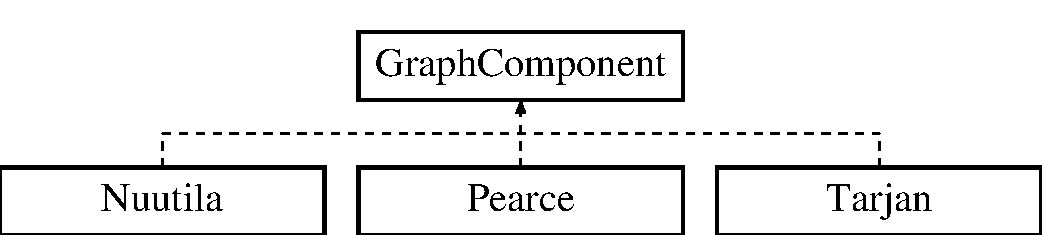
\includegraphics[height=2.000000cm]{class_graph_component}
\end{center}
\end{figure}
\subsection*{Public Types}
\begin{DoxyCompactItemize}
\item 
typedef \hyperlink{struct_utility_structs_1_1_vertex_property}{Utility\+Structs\+::\+Vertex\+Property} \hyperlink{class_graph_component_a7c0fcb3f03bf188b7df520e0cdd364b7}{Vertex\+Property}
\item 
typedef \hyperlink{struct_utility_structs_1_1_edge_property}{Utility\+Structs\+::\+Edge\+Property} \hyperlink{class_graph_component_ae2f6ef4a3ac656d8213df42aa3d4c3b3}{Edge\+Property}
\item 
typedef boost\+::adjacency\+\_\+list$<$ boost\+::vecS, boost\+::listS, boost\+::directedS, \hyperlink{class_graph_component_a7c0fcb3f03bf188b7df520e0cdd364b7}{Vertex\+Property}, \hyperlink{class_graph_component_ae2f6ef4a3ac656d8213df42aa3d4c3b3}{Edge\+Property} $>$ \hyperlink{class_graph_component_a982e0748a6e1b8dc74986f5f8b3dca5c}{the\+Graph}
\item 
typedef boost\+::graph\+\_\+traits$<$ \hyperlink{class_graph_component_a982e0748a6e1b8dc74986f5f8b3dca5c}{the\+Graph} $>$\+::vertex\+\_\+descriptor \hyperlink{class_graph_component_ae67114a6ce5a001dc35e1996e1b45aa0}{Vertex\+\_\+t}
\item 
typedef boost\+::graph\+\_\+traits$<$ \hyperlink{class_graph_component_a982e0748a6e1b8dc74986f5f8b3dca5c}{the\+Graph} $>$\+::edge\+\_\+descriptor \hyperlink{class_graph_component_aa7517b2af08aa717324076a645c73fe6}{Edge}
\item 
typedef property\+\_\+map$<$ \hyperlink{class_graph_component_a982e0748a6e1b8dc74986f5f8b3dca5c}{the\+Graph}, std\+::size\+\_\+t Vertex\+Property\+::$\ast$ $>$\+::type \hyperlink{class_graph_component_ad40772702161324303e24463a63738e9}{v\+\_\+p}
\item 
typedef property\+\_\+map$<$ \hyperlink{class_graph_component_a982e0748a6e1b8dc74986f5f8b3dca5c}{the\+Graph}, std\+::string Edge\+Property\+::$\ast$ $>$\+::type \hyperlink{class_graph_component_a22292bf7520fb476958c508d66f5d318}{e\+\_\+p}
\end{DoxyCompactItemize}
\subsection*{Public Member Functions}
\begin{DoxyCompactItemize}
\item 
\hyperlink{class_graph_component_a35c4a6e5c6f28751b1bd6c451cc07957}{Graph\+Component} ()
\item 
\hyperlink{class_graph_component_a14482fdab4e309677b4a14ab8db13079}{Graph\+Component} (std\+::string filename)
\item 
void \hyperlink{class_graph_component_a6af293dac3774fde0e2822b5725ecacd}{print\+\_\+graph\+\_\+file} (\hyperlink{class_graph_component_a982e0748a6e1b8dc74986f5f8b3dca5c}{the\+Graph} \&graph)
\item 
void \hyperlink{class_graph_component_a680363eab8b992d739f055bd484bc000}{read\+\_\+graph\+\_\+file} (std\+::string filename, \hyperlink{class_graph_component_a982e0748a6e1b8dc74986f5f8b3dca5c}{the\+Graph} \&g)
\end{DoxyCompactItemize}


\subsection{Detailed Description}
This class is used to read graphs from the file and import them to the Boost Graph objects. 

It also contains a graph printing function which can work with small graphs but after some point the screen size is not enough 

\subsection{Member Typedef Documentation}
\mbox{\Hypertarget{class_graph_component_a22292bf7520fb476958c508d66f5d318}\label{class_graph_component_a22292bf7520fb476958c508d66f5d318}} 
\index{Graph\+Component@{Graph\+Component}!e\+\_\+p@{e\+\_\+p}}
\index{e\+\_\+p@{e\+\_\+p}!Graph\+Component@{Graph\+Component}}
\subsubsection{\texorpdfstring{e\+\_\+p}{e\_p}}
{\footnotesize\ttfamily typedef property\+\_\+map$<$\hyperlink{class_graph_component_a982e0748a6e1b8dc74986f5f8b3dca5c}{the\+Graph}, std\+::string Edge\+Property\+::$\ast$$>$\+::type \hyperlink{class_graph_component_a22292bf7520fb476958c508d66f5d318}{Graph\+Component\+::e\+\_\+p}}

\mbox{\Hypertarget{class_graph_component_aa7517b2af08aa717324076a645c73fe6}\label{class_graph_component_aa7517b2af08aa717324076a645c73fe6}} 
\index{Graph\+Component@{Graph\+Component}!Edge@{Edge}}
\index{Edge@{Edge}!Graph\+Component@{Graph\+Component}}
\subsubsection{\texorpdfstring{Edge}{Edge}}
{\footnotesize\ttfamily typedef boost\+::graph\+\_\+traits$<$\hyperlink{class_graph_component_a982e0748a6e1b8dc74986f5f8b3dca5c}{the\+Graph}$>$\+::edge\+\_\+descriptor \hyperlink{class_graph_component_aa7517b2af08aa717324076a645c73fe6}{Graph\+Component\+::\+Edge}}

\mbox{\Hypertarget{class_graph_component_ae2f6ef4a3ac656d8213df42aa3d4c3b3}\label{class_graph_component_ae2f6ef4a3ac656d8213df42aa3d4c3b3}} 
\index{Graph\+Component@{Graph\+Component}!Edge\+Property@{Edge\+Property}}
\index{Edge\+Property@{Edge\+Property}!Graph\+Component@{Graph\+Component}}
\subsubsection{\texorpdfstring{Edge\+Property}{EdgeProperty}}
{\footnotesize\ttfamily typedef \hyperlink{struct_utility_structs_1_1_edge_property}{Utility\+Structs\+::\+Edge\+Property} \hyperlink{class_graph_component_ae2f6ef4a3ac656d8213df42aa3d4c3b3}{Graph\+Component\+::\+Edge\+Property}}

\mbox{\Hypertarget{class_graph_component_a982e0748a6e1b8dc74986f5f8b3dca5c}\label{class_graph_component_a982e0748a6e1b8dc74986f5f8b3dca5c}} 
\index{Graph\+Component@{Graph\+Component}!the\+Graph@{the\+Graph}}
\index{the\+Graph@{the\+Graph}!Graph\+Component@{Graph\+Component}}
\subsubsection{\texorpdfstring{the\+Graph}{theGraph}}
{\footnotesize\ttfamily typedef boost\+::adjacency\+\_\+list$<$boost\+::vecS, boost\+::listS, boost\+::directedS, \hyperlink{class_graph_component_a7c0fcb3f03bf188b7df520e0cdd364b7}{Vertex\+Property}, \hyperlink{class_graph_component_ae2f6ef4a3ac656d8213df42aa3d4c3b3}{Edge\+Property}$>$ \hyperlink{class_graph_component_a982e0748a6e1b8dc74986f5f8b3dca5c}{Graph\+Component\+::the\+Graph}}

\mbox{\Hypertarget{class_graph_component_ad40772702161324303e24463a63738e9}\label{class_graph_component_ad40772702161324303e24463a63738e9}} 
\index{Graph\+Component@{Graph\+Component}!v\+\_\+p@{v\+\_\+p}}
\index{v\+\_\+p@{v\+\_\+p}!Graph\+Component@{Graph\+Component}}
\subsubsection{\texorpdfstring{v\+\_\+p}{v\_p}}
{\footnotesize\ttfamily typedef property\+\_\+map$<$\hyperlink{class_graph_component_a982e0748a6e1b8dc74986f5f8b3dca5c}{the\+Graph}, std\+::size\+\_\+t Vertex\+Property\+::$\ast$$>$\+::type \hyperlink{class_graph_component_ad40772702161324303e24463a63738e9}{Graph\+Component\+::v\+\_\+p}}

\mbox{\Hypertarget{class_graph_component_ae67114a6ce5a001dc35e1996e1b45aa0}\label{class_graph_component_ae67114a6ce5a001dc35e1996e1b45aa0}} 
\index{Graph\+Component@{Graph\+Component}!Vertex\+\_\+t@{Vertex\+\_\+t}}
\index{Vertex\+\_\+t@{Vertex\+\_\+t}!Graph\+Component@{Graph\+Component}}
\subsubsection{\texorpdfstring{Vertex\+\_\+t}{Vertex\_t}}
{\footnotesize\ttfamily typedef boost\+::graph\+\_\+traits$<$\hyperlink{class_graph_component_a982e0748a6e1b8dc74986f5f8b3dca5c}{the\+Graph}$>$\+::vertex\+\_\+descriptor \hyperlink{class_graph_component_ae67114a6ce5a001dc35e1996e1b45aa0}{Graph\+Component\+::\+Vertex\+\_\+t}}

\mbox{\Hypertarget{class_graph_component_a7c0fcb3f03bf188b7df520e0cdd364b7}\label{class_graph_component_a7c0fcb3f03bf188b7df520e0cdd364b7}} 
\index{Graph\+Component@{Graph\+Component}!Vertex\+Property@{Vertex\+Property}}
\index{Vertex\+Property@{Vertex\+Property}!Graph\+Component@{Graph\+Component}}
\subsubsection{\texorpdfstring{Vertex\+Property}{VertexProperty}}
{\footnotesize\ttfamily typedef \hyperlink{struct_utility_structs_1_1_vertex_property}{Utility\+Structs\+::\+Vertex\+Property} \hyperlink{class_graph_component_a7c0fcb3f03bf188b7df520e0cdd364b7}{Graph\+Component\+::\+Vertex\+Property}}



\subsection{Constructor \& Destructor Documentation}
\mbox{\Hypertarget{class_graph_component_a35c4a6e5c6f28751b1bd6c451cc07957}\label{class_graph_component_a35c4a6e5c6f28751b1bd6c451cc07957}} 
\index{Graph\+Component@{Graph\+Component}!Graph\+Component@{Graph\+Component}}
\index{Graph\+Component@{Graph\+Component}!Graph\+Component@{Graph\+Component}}
\subsubsection{\texorpdfstring{Graph\+Component()}{GraphComponent()}\hspace{0.1cm}{\footnotesize\ttfamily [1/2]}}
{\footnotesize\ttfamily Graph\+Component\+::\+Graph\+Component (\begin{DoxyParamCaption}{ }\end{DoxyParamCaption})}

\mbox{\Hypertarget{class_graph_component_a14482fdab4e309677b4a14ab8db13079}\label{class_graph_component_a14482fdab4e309677b4a14ab8db13079}} 
\index{Graph\+Component@{Graph\+Component}!Graph\+Component@{Graph\+Component}}
\index{Graph\+Component@{Graph\+Component}!Graph\+Component@{Graph\+Component}}
\subsubsection{\texorpdfstring{Graph\+Component()}{GraphComponent()}\hspace{0.1cm}{\footnotesize\ttfamily [2/2]}}
{\footnotesize\ttfamily Graph\+Component\+::\+Graph\+Component (\begin{DoxyParamCaption}\item[{std\+::string}]{filename }\end{DoxyParamCaption})\hspace{0.3cm}{\ttfamily [inline]}}



\subsection{Member Function Documentation}
\mbox{\Hypertarget{class_graph_component_a6af293dac3774fde0e2822b5725ecacd}\label{class_graph_component_a6af293dac3774fde0e2822b5725ecacd}} 
\index{Graph\+Component@{Graph\+Component}!print\+\_\+graph\+\_\+file@{print\+\_\+graph\+\_\+file}}
\index{print\+\_\+graph\+\_\+file@{print\+\_\+graph\+\_\+file}!Graph\+Component@{Graph\+Component}}
\subsubsection{\texorpdfstring{print\+\_\+graph\+\_\+file()}{print\_graph\_file()}}
{\footnotesize\ttfamily void Graph\+Component\+::print\+\_\+graph\+\_\+file (\begin{DoxyParamCaption}\item[{\hyperlink{class_graph_component_a982e0748a6e1b8dc74986f5f8b3dca5c}{the\+Graph} \&}]{graph }\end{DoxyParamCaption})}

\mbox{\Hypertarget{class_graph_component_a680363eab8b992d739f055bd484bc000}\label{class_graph_component_a680363eab8b992d739f055bd484bc000}} 
\index{Graph\+Component@{Graph\+Component}!read\+\_\+graph\+\_\+file@{read\+\_\+graph\+\_\+file}}
\index{read\+\_\+graph\+\_\+file@{read\+\_\+graph\+\_\+file}!Graph\+Component@{Graph\+Component}}
\subsubsection{\texorpdfstring{read\+\_\+graph\+\_\+file()}{read\_graph\_file()}}
{\footnotesize\ttfamily void Graph\+Component\+::read\+\_\+graph\+\_\+file (\begin{DoxyParamCaption}\item[{std\+::string}]{filename,  }\item[{\hyperlink{class_graph_component_a982e0748a6e1b8dc74986f5f8b3dca5c}{the\+Graph} \&}]{g }\end{DoxyParamCaption})}



The documentation for this class was generated from the following file\+:\begin{DoxyCompactItemize}
\item 
header/\hyperlink{graphcomponent_8h}{graphcomponent.\+h}\end{DoxyCompactItemize}

\hypertarget{class_nuutila}{}\section{Nuutila Class Reference}
\label{class_nuutila}\index{Nuutila@{Nuutila}}


This class contains the implementations of algorithms from the \hyperlink{class_nuutila}{Nuutila}\textquotesingle{}s Paper.  




{\ttfamily \#include $<$nuutila.\+h$>$}

Inheritance diagram for Nuutila\+:\begin{figure}[H]
\begin{center}
\leavevmode
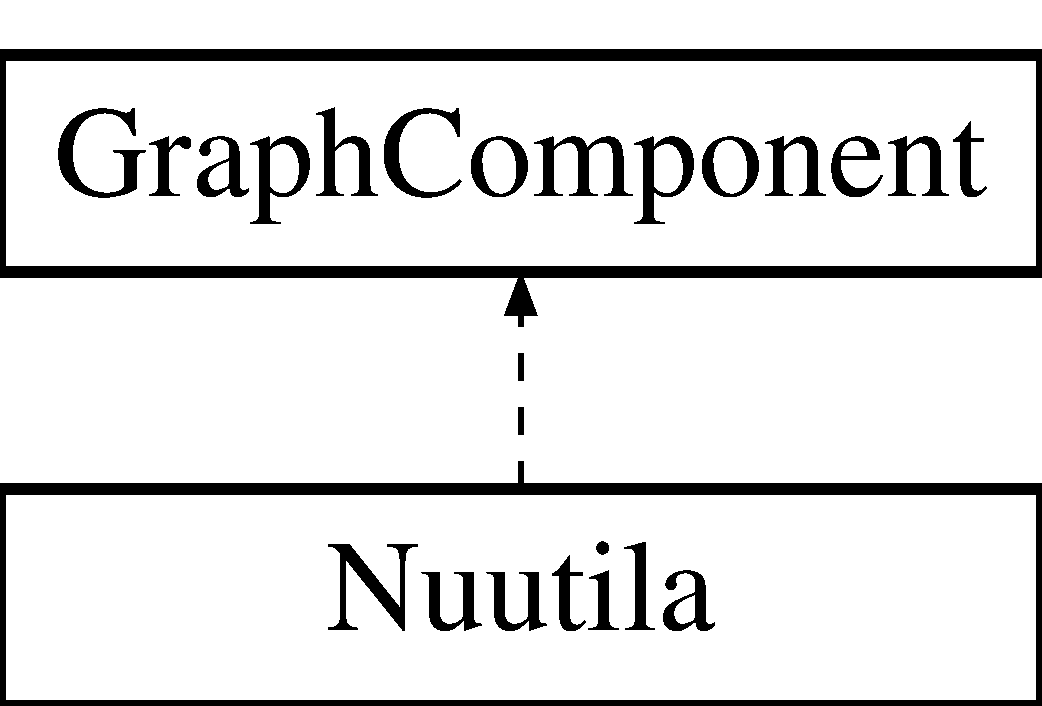
\includegraphics[height=2.000000cm]{class_nuutila}
\end{center}
\end{figure}
\subsection*{Public Member Functions}
\begin{DoxyCompactItemize}
\item 
\hyperlink{class_nuutila_ab1ae0281145f693a922f5122d27cc23b}{Nuutila} ()
\item 
\hyperlink{class_nuutila_a00bb9066a5a1c9fb03e25481f4f47a0c}{Nuutila} (std\+::string filename)
\item 
void \hyperlink{class_nuutila_ae56bd15d2e57366eef0e044bf3a37d9e}{solve} (std\+::vector$<$ std\+::string $>$ methods, int graph\+Num)
\item 
void \hyperlink{class_nuutila_ae11b94c396dff5b8d9b7f69ae0d0831f}{print\+\_\+sccs} (\hyperlink{struct_utility_structs_1_1_storage_items}{Utility\+Structs\+::\+Storage\+Items} \&s)
\item 
void \hyperlink{class_nuutila_a0dc1cb3d0711a856a32a3743a85fb5c8}{print\+\_\+graph} ()
\item 
\hyperlink{struct_utility_structs_1_1_storage_items}{Utility\+Structs\+::\+Storage\+Items} \hyperlink{class_nuutila_a7d52f96cf25409704bfd7bf176fcc7c5}{Apply\+S\+C\+C\+\_\+\+Original} ()
\item 
void \hyperlink{class_nuutila_a2d43bc514d7375f9d63e60c06f90a60f}{Visit} (\hyperlink{class_graph_component_ae67114a6ce5a001dc35e1996e1b45aa0}{Vertex\+\_\+t} \&v, std\+::vector$<$ \hyperlink{class_graph_component_ae67114a6ce5a001dc35e1996e1b45aa0}{Vertex\+\_\+t} $>$ \&Points, std\+::vector$<$ int $>$ \&root, std\+::vector$<$ int $>$ \&visited, std\+::vector$<$ bool $>$ \&is\+Component, int \&Counter, int \&stack\+Count)
\item 
\hyperlink{struct_utility_structs_1_1_storage_items}{Utility\+Structs\+::\+Storage\+Items} \hyperlink{class_nuutila_a6c355594f68dad8c28684114a6df6700}{Apply\+S\+C\+C\+\_\+v1} ()
\item 
\hyperlink{struct_utility_structs_1_1_storage_items}{Utility\+Structs\+::\+Storage\+Items} \hyperlink{class_nuutila_a291d578f760e0f11a5c56c8a5fe02ebd}{Apply\+S\+C\+C\+\_\+v2} ()
\item 
void \hyperlink{class_nuutila_a83b47177cf452e80b3ceaf064ff59840}{Visit\+\_\+v1} (\hyperlink{class_graph_component_ae67114a6ce5a001dc35e1996e1b45aa0}{Vertex\+\_\+t} \&v, std\+::vector$<$ \hyperlink{class_graph_component_ae67114a6ce5a001dc35e1996e1b45aa0}{Vertex\+\_\+t} $>$ \&Points, std\+::vector$<$ int $>$ \&root, std\+::vector$<$ int $>$ \&visited, std\+::vector$<$ bool $>$ \&is\+Component, int \&Counter, int \&stack\+Count)
\item 
void \hyperlink{class_nuutila_afc7a8c27d8de17ac2679f839ff8c2749}{Visit\+\_\+v2} (\hyperlink{class_graph_component_ae67114a6ce5a001dc35e1996e1b45aa0}{Vertex\+\_\+t} \&v, std\+::vector$<$ int $>$ \&Points, std\+::vector$<$ int $>$ \&root, std\+::vector$<$ int $>$ \&visited, std\+::vector$<$ bool $>$ \&is\+Component, int \&Counter, int \&stack\+Count)
\end{DoxyCompactItemize}
\subsection*{Public Attributes}
\begin{DoxyCompactItemize}
\item 
\hyperlink{class_graph_component_a982e0748a6e1b8dc74986f5f8b3dca5c}{the\+Graph} \hyperlink{class_nuutila_a1409929fa0f38709497f8bdb012af71c}{n}
\item 
std\+::vector$<$ \hyperlink{class_graph_component_a982e0748a6e1b8dc74986f5f8b3dca5c}{the\+Graph} $>$ \hyperlink{class_nuutila_a70e8a910cc4050d246db2540bd1e36c5}{experiment}
\end{DoxyCompactItemize}
\subsection*{Additional Inherited Members}


\subsection{Detailed Description}
This class contains the implementations of algorithms from the \hyperlink{class_nuutila}{Nuutila}\textquotesingle{}s Paper. 

\subsection{Constructor \& Destructor Documentation}
\mbox{\Hypertarget{class_nuutila_ab1ae0281145f693a922f5122d27cc23b}\label{class_nuutila_ab1ae0281145f693a922f5122d27cc23b}} 
\index{Nuutila@{Nuutila}!Nuutila@{Nuutila}}
\index{Nuutila@{Nuutila}!Nuutila@{Nuutila}}
\subsubsection{\texorpdfstring{Nuutila()}{Nuutila()}\hspace{0.1cm}{\footnotesize\ttfamily [1/2]}}
{\footnotesize\ttfamily Nuutila\+::\+Nuutila (\begin{DoxyParamCaption}{ }\end{DoxyParamCaption})\hspace{0.3cm}{\ttfamily [inline]}}

\mbox{\Hypertarget{class_nuutila_a00bb9066a5a1c9fb03e25481f4f47a0c}\label{class_nuutila_a00bb9066a5a1c9fb03e25481f4f47a0c}} 
\index{Nuutila@{Nuutila}!Nuutila@{Nuutila}}
\index{Nuutila@{Nuutila}!Nuutila@{Nuutila}}
\subsubsection{\texorpdfstring{Nuutila()}{Nuutila()}\hspace{0.1cm}{\footnotesize\ttfamily [2/2]}}
{\footnotesize\ttfamily Nuutila\+::\+Nuutila (\begin{DoxyParamCaption}\item[{std\+::string}]{filename }\end{DoxyParamCaption})\hspace{0.3cm}{\ttfamily [inline]}}



\subsection{Member Function Documentation}
\mbox{\Hypertarget{class_nuutila_a7d52f96cf25409704bfd7bf176fcc7c5}\label{class_nuutila_a7d52f96cf25409704bfd7bf176fcc7c5}} 
\index{Nuutila@{Nuutila}!Apply\+S\+C\+C\+\_\+\+Original@{Apply\+S\+C\+C\+\_\+\+Original}}
\index{Apply\+S\+C\+C\+\_\+\+Original@{Apply\+S\+C\+C\+\_\+\+Original}!Nuutila@{Nuutila}}
\subsubsection{\texorpdfstring{Apply\+S\+C\+C\+\_\+\+Original()}{ApplySCC\_Original()}}
{\footnotesize\ttfamily \hyperlink{struct_utility_structs_1_1_storage_items}{Utility\+Structs\+::\+Storage\+Items} Nuutila\+::\+Apply\+S\+C\+C\+\_\+\+Original (\begin{DoxyParamCaption}{ }\end{DoxyParamCaption})}

\mbox{\Hypertarget{class_nuutila_a6c355594f68dad8c28684114a6df6700}\label{class_nuutila_a6c355594f68dad8c28684114a6df6700}} 
\index{Nuutila@{Nuutila}!Apply\+S\+C\+C\+\_\+v1@{Apply\+S\+C\+C\+\_\+v1}}
\index{Apply\+S\+C\+C\+\_\+v1@{Apply\+S\+C\+C\+\_\+v1}!Nuutila@{Nuutila}}
\subsubsection{\texorpdfstring{Apply\+S\+C\+C\+\_\+v1()}{ApplySCC\_v1()}}
{\footnotesize\ttfamily \hyperlink{struct_utility_structs_1_1_storage_items}{Utility\+Structs\+::\+Storage\+Items} Nuutila\+::\+Apply\+S\+C\+C\+\_\+v1 (\begin{DoxyParamCaption}{ }\end{DoxyParamCaption})}

\mbox{\Hypertarget{class_nuutila_a291d578f760e0f11a5c56c8a5fe02ebd}\label{class_nuutila_a291d578f760e0f11a5c56c8a5fe02ebd}} 
\index{Nuutila@{Nuutila}!Apply\+S\+C\+C\+\_\+v2@{Apply\+S\+C\+C\+\_\+v2}}
\index{Apply\+S\+C\+C\+\_\+v2@{Apply\+S\+C\+C\+\_\+v2}!Nuutila@{Nuutila}}
\subsubsection{\texorpdfstring{Apply\+S\+C\+C\+\_\+v2()}{ApplySCC\_v2()}}
{\footnotesize\ttfamily \hyperlink{struct_utility_structs_1_1_storage_items}{Utility\+Structs\+::\+Storage\+Items} Nuutila\+::\+Apply\+S\+C\+C\+\_\+v2 (\begin{DoxyParamCaption}{ }\end{DoxyParamCaption})}

\mbox{\Hypertarget{class_nuutila_a0dc1cb3d0711a856a32a3743a85fb5c8}\label{class_nuutila_a0dc1cb3d0711a856a32a3743a85fb5c8}} 
\index{Nuutila@{Nuutila}!print\+\_\+graph@{print\+\_\+graph}}
\index{print\+\_\+graph@{print\+\_\+graph}!Nuutila@{Nuutila}}
\subsubsection{\texorpdfstring{print\+\_\+graph()}{print\_graph()}}
{\footnotesize\ttfamily void Nuutila\+::print\+\_\+graph (\begin{DoxyParamCaption}{ }\end{DoxyParamCaption})}

\mbox{\Hypertarget{class_nuutila_ae11b94c396dff5b8d9b7f69ae0d0831f}\label{class_nuutila_ae11b94c396dff5b8d9b7f69ae0d0831f}} 
\index{Nuutila@{Nuutila}!print\+\_\+sccs@{print\+\_\+sccs}}
\index{print\+\_\+sccs@{print\+\_\+sccs}!Nuutila@{Nuutila}}
\subsubsection{\texorpdfstring{print\+\_\+sccs()}{print\_sccs()}}
{\footnotesize\ttfamily void Nuutila\+::print\+\_\+sccs (\begin{DoxyParamCaption}\item[{\hyperlink{struct_utility_structs_1_1_storage_items}{Utility\+Structs\+::\+Storage\+Items} \&}]{s }\end{DoxyParamCaption})}

\mbox{\Hypertarget{class_nuutila_ae56bd15d2e57366eef0e044bf3a37d9e}\label{class_nuutila_ae56bd15d2e57366eef0e044bf3a37d9e}} 
\index{Nuutila@{Nuutila}!solve@{solve}}
\index{solve@{solve}!Nuutila@{Nuutila}}
\subsubsection{\texorpdfstring{solve()}{solve()}}
{\footnotesize\ttfamily void Nuutila\+::solve (\begin{DoxyParamCaption}\item[{std\+::vector$<$ std\+::string $>$}]{methods,  }\item[{int}]{graph\+Num }\end{DoxyParamCaption})}

\mbox{\Hypertarget{class_nuutila_a2d43bc514d7375f9d63e60c06f90a60f}\label{class_nuutila_a2d43bc514d7375f9d63e60c06f90a60f}} 
\index{Nuutila@{Nuutila}!Visit@{Visit}}
\index{Visit@{Visit}!Nuutila@{Nuutila}}
\subsubsection{\texorpdfstring{Visit()}{Visit()}}
{\footnotesize\ttfamily void Nuutila\+::\+Visit (\begin{DoxyParamCaption}\item[{\hyperlink{class_graph_component_ae67114a6ce5a001dc35e1996e1b45aa0}{Vertex\+\_\+t} \&}]{v,  }\item[{std\+::vector$<$ \hyperlink{class_graph_component_ae67114a6ce5a001dc35e1996e1b45aa0}{Vertex\+\_\+t} $>$ \&}]{Points,  }\item[{std\+::vector$<$ int $>$ \&}]{root,  }\item[{std\+::vector$<$ int $>$ \&}]{visited,  }\item[{std\+::vector$<$ bool $>$ \&}]{is\+Component,  }\item[{int \&}]{Counter,  }\item[{int \&}]{stack\+Count }\end{DoxyParamCaption})}

\mbox{\Hypertarget{class_nuutila_a83b47177cf452e80b3ceaf064ff59840}\label{class_nuutila_a83b47177cf452e80b3ceaf064ff59840}} 
\index{Nuutila@{Nuutila}!Visit\+\_\+v1@{Visit\+\_\+v1}}
\index{Visit\+\_\+v1@{Visit\+\_\+v1}!Nuutila@{Nuutila}}
\subsubsection{\texorpdfstring{Visit\+\_\+v1()}{Visit\_v1()}}
{\footnotesize\ttfamily void Nuutila\+::\+Visit\+\_\+v1 (\begin{DoxyParamCaption}\item[{\hyperlink{class_graph_component_ae67114a6ce5a001dc35e1996e1b45aa0}{Vertex\+\_\+t} \&}]{v,  }\item[{std\+::vector$<$ \hyperlink{class_graph_component_ae67114a6ce5a001dc35e1996e1b45aa0}{Vertex\+\_\+t} $>$ \&}]{Points,  }\item[{std\+::vector$<$ int $>$ \&}]{root,  }\item[{std\+::vector$<$ int $>$ \&}]{visited,  }\item[{std\+::vector$<$ bool $>$ \&}]{is\+Component,  }\item[{int \&}]{Counter,  }\item[{int \&}]{stack\+Count }\end{DoxyParamCaption})}

\mbox{\Hypertarget{class_nuutila_afc7a8c27d8de17ac2679f839ff8c2749}\label{class_nuutila_afc7a8c27d8de17ac2679f839ff8c2749}} 
\index{Nuutila@{Nuutila}!Visit\+\_\+v2@{Visit\+\_\+v2}}
\index{Visit\+\_\+v2@{Visit\+\_\+v2}!Nuutila@{Nuutila}}
\subsubsection{\texorpdfstring{Visit\+\_\+v2()}{Visit\_v2()}}
{\footnotesize\ttfamily void Nuutila\+::\+Visit\+\_\+v2 (\begin{DoxyParamCaption}\item[{\hyperlink{class_graph_component_ae67114a6ce5a001dc35e1996e1b45aa0}{Vertex\+\_\+t} \&}]{v,  }\item[{std\+::vector$<$ int $>$ \&}]{Points,  }\item[{std\+::vector$<$ int $>$ \&}]{root,  }\item[{std\+::vector$<$ int $>$ \&}]{visited,  }\item[{std\+::vector$<$ bool $>$ \&}]{is\+Component,  }\item[{int \&}]{Counter,  }\item[{int \&}]{stack\+Count }\end{DoxyParamCaption})}



\subsection{Member Data Documentation}
\mbox{\Hypertarget{class_nuutila_a70e8a910cc4050d246db2540bd1e36c5}\label{class_nuutila_a70e8a910cc4050d246db2540bd1e36c5}} 
\index{Nuutila@{Nuutila}!experiment@{experiment}}
\index{experiment@{experiment}!Nuutila@{Nuutila}}
\subsubsection{\texorpdfstring{experiment}{experiment}}
{\footnotesize\ttfamily std\+::vector$<$\hyperlink{class_graph_component_a982e0748a6e1b8dc74986f5f8b3dca5c}{the\+Graph}$>$ Nuutila\+::experiment}

\mbox{\Hypertarget{class_nuutila_a1409929fa0f38709497f8bdb012af71c}\label{class_nuutila_a1409929fa0f38709497f8bdb012af71c}} 
\index{Nuutila@{Nuutila}!n@{n}}
\index{n@{n}!Nuutila@{Nuutila}}
\subsubsection{\texorpdfstring{n}{n}}
{\footnotesize\ttfamily \hyperlink{class_graph_component_a982e0748a6e1b8dc74986f5f8b3dca5c}{the\+Graph} Nuutila\+::n}



The documentation for this class was generated from the following file\+:\begin{DoxyCompactItemize}
\item 
header/\hyperlink{nuutila_8h}{nuutila.\+h}\end{DoxyCompactItemize}

\hypertarget{class_pearce}{}\section{Pearce Class Reference}
\label{class_pearce}\index{Pearce@{Pearce}}


{\ttfamily \#include $<$pearce.\+h$>$}

Inheritance diagram for Pearce\+:\begin{figure}[H]
\begin{center}
\leavevmode
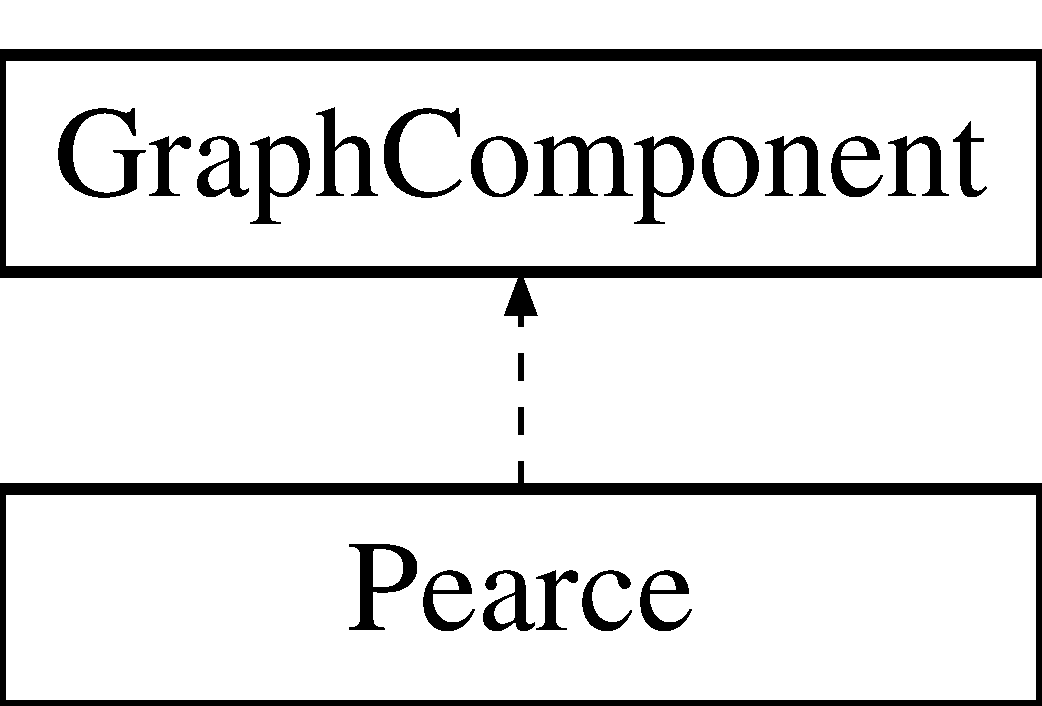
\includegraphics[height=2.000000cm]{class_pearce}
\end{center}
\end{figure}
\subsection*{Public Member Functions}
\begin{DoxyCompactItemize}
\item 
\hyperlink{class_pearce_a4ad24a40c64e8f3481dd0dbbcb8d2bcb_a4ad24a40c64e8f3481dd0dbbcb8d2bcb}{Pearce} ()=default
\item 
\hyperlink{class_pearce_a0851b1b696528448c1a42dbb6b4e6c8f_a0851b1b696528448c1a42dbb6b4e6c8f}{Pearce} (std\+::string filename)
\item 
void \hyperlink{class_pearce_a7c6ea7dde3dc3e127e4fc6ad1892974e_a7c6ea7dde3dc3e127e4fc6ad1892974e}{solve} (std\+::vector$<$ std\+::string $>$ methods, int graph\+Num)
\item 
void \hyperlink{class_pearce_a96ed7e50d992838177699b6133464554_a96ed7e50d992838177699b6133464554}{print\+\_\+graph} ()
\item 
void \hyperlink{class_pearce_aaa906779c670a16948c00a9c031e6986_aaa906779c670a16948c00a9c031e6986}{print\+\_\+result\+\_\+max} (\hyperlink{struct_utility_structs_1_1_storage_items}{Utility\+Structs\+::\+Storage\+Items} \&s)
\item 
void \hyperlink{class_pearce_af2a6f31643617305794c06b5d2c85ebe_af2a6f31643617305794c06b5d2c85ebe}{print\+\_\+result\+\_\+min} (\hyperlink{struct_utility_structs_1_1_storage_items}{Utility\+Structs\+::\+Storage\+Items} \&s)
\item 
void \hyperlink{class_pearce_ad50f62a493ed2b5eb7fcb3c0f8e2e079_ad50f62a493ed2b5eb7fcb3c0f8e2e079}{D\+FS} ()
\item 
void \hyperlink{class_pearce_ac5e668d0d21ee0dad33cea171b9e2022_ac5e668d0d21ee0dad33cea171b9e2022}{visit} (\hyperlink{class_graph_component_ae67114a6ce5a001dc35e1996e1b45aa0_ae67114a6ce5a001dc35e1996e1b45aa0}{Vertex\+\_\+t} \&v, std\+::vector$<$ int $>$ \&visited, int \&index)
\item 
\hyperlink{struct_utility_structs_1_1_storage_items}{Utility\+Structs\+::\+Storage\+Items} \hyperlink{class_pearce_a4a78c1ec037146537f575fa62b1e0265_a4a78c1ec037146537f575fa62b1e0265}{Pea\+\_\+\+Find\+\_\+\+S\+C\+C1} ()
\item 
void \hyperlink{class_pearce_ae4e9364dd0c829564ecfbfe8ccc07b6a_ae4e9364dd0c829564ecfbfe8ccc07b6a}{visit\+\_\+scc1} (\hyperlink{class_graph_component_ae67114a6ce5a001dc35e1996e1b45aa0_ae67114a6ce5a001dc35e1996e1b45aa0}{Vertex\+\_\+t} \&v, std\+::vector$<$ bool $>$ \&visited, std\+::vector$<$ int $>$ \&rindex, std\+::vector$<$ bool $>$ \&in\+Component, std\+::vector$<$ \hyperlink{class_graph_component_ae67114a6ce5a001dc35e1996e1b45aa0_ae67114a6ce5a001dc35e1996e1b45aa0}{Vertex\+\_\+t} $>$ \&Stack, int \&index, int \&c, int \&stack\+Count)
\item 
\hyperlink{struct_utility_structs_1_1_storage_items}{Utility\+Structs\+::\+Storage\+Items} \hyperlink{class_pearce_a4764238b69ee587134a9009619a4cae5_a4764238b69ee587134a9009619a4cae5}{Pea\+\_\+\+Find\+\_\+\+S\+C\+C2} ()
\item 
void \hyperlink{class_pearce_a12c836f8f0dbd85e20c0f3f4f0c5fb47_a12c836f8f0dbd85e20c0f3f4f0c5fb47}{visit\+\_\+scc2} (\hyperlink{class_graph_component_ae67114a6ce5a001dc35e1996e1b45aa0_ae67114a6ce5a001dc35e1996e1b45aa0}{Vertex\+\_\+t} \&v, std\+::vector$<$ int $>$ \&rindex, std\+::vector$<$ \hyperlink{class_graph_component_ae67114a6ce5a001dc35e1996e1b45aa0_ae67114a6ce5a001dc35e1996e1b45aa0}{Vertex\+\_\+t} $>$ \&Stack, int \&index, int \&c, int \&stack\+Count)
\item 
\hyperlink{struct_utility_structs_1_1_storage_items}{Utility\+Structs\+::\+Storage\+Items} \hyperlink{class_pearce_a9d49726ab058f24cc943135458edb4f9_a9d49726ab058f24cc943135458edb4f9}{Pea\+\_\+\+Find\+\_\+\+S\+C\+C3} ()
\item 
void \hyperlink{class_pearce_a70800d4564b36fb64762d3a78f1f67d8_a70800d4564b36fb64762d3a78f1f67d8}{visit\+\_\+scc3} (\hyperlink{class_graph_component_ae67114a6ce5a001dc35e1996e1b45aa0_ae67114a6ce5a001dc35e1996e1b45aa0}{Vertex\+\_\+t} \&v, std\+::vector$<$ bool $>$ \&root, std\+::vector$<$ int $>$ \&rindex, std\+::vector$<$ \hyperlink{class_graph_component_ae67114a6ce5a001dc35e1996e1b45aa0_ae67114a6ce5a001dc35e1996e1b45aa0}{Vertex\+\_\+t} $>$ \&v\+Stack, std\+::vector$<$ int $>$ \&i\+Stack, int \&index, int \&c, int \&stack\+Count\+\_\+i, int \&stack\+Count\+\_\+v)
\item 
void \hyperlink{class_pearce_a323fc3337d5849680065986d6ef7163c_a323fc3337d5849680065986d6ef7163c}{visit\+Loop} (std\+::vector$<$ bool $>$ \&root, std\+::vector$<$ int $>$ \&rindex, std\+::vector$<$ \hyperlink{class_graph_component_ae67114a6ce5a001dc35e1996e1b45aa0_ae67114a6ce5a001dc35e1996e1b45aa0}{Vertex\+\_\+t} $>$ \&v\+Stack, std\+::vector$<$ int $>$ \&i\+Stack, int \&index, int \&c, int \&stack\+Count\+\_\+i, int \&stack\+Count\+\_\+v)
\item 
void \hyperlink{class_pearce_ab9090eeb4466701bc8ba913d8f9f5b50_ab9090eeb4466701bc8ba913d8f9f5b50}{begin\+Visiting} (\hyperlink{class_graph_component_ae67114a6ce5a001dc35e1996e1b45aa0_ae67114a6ce5a001dc35e1996e1b45aa0}{Vertex\+\_\+t} \&v, std\+::vector$<$ bool $>$ \&root, std\+::vector$<$ int $>$ \&rindex, std\+::vector$<$ \hyperlink{class_graph_component_ae67114a6ce5a001dc35e1996e1b45aa0_ae67114a6ce5a001dc35e1996e1b45aa0}{Vertex\+\_\+t} $>$ \&v\+Stack, std\+::vector$<$ int $>$ \&i\+Stack, int \&index, int \&stack\+Count\+\_\+i, int \&stack\+Count\+\_\+v)
\item 
void \hyperlink{class_pearce_a48afb6ccb75ba9df285c9701daf474b0_a48afb6ccb75ba9df285c9701daf474b0}{finish\+Visiting} (\hyperlink{class_graph_component_ae67114a6ce5a001dc35e1996e1b45aa0_ae67114a6ce5a001dc35e1996e1b45aa0}{Vertex\+\_\+t} \&v, std\+::vector$<$ bool $>$ \&root, std\+::vector$<$ int $>$ \&rindex, std\+::vector$<$ \hyperlink{class_graph_component_ae67114a6ce5a001dc35e1996e1b45aa0_ae67114a6ce5a001dc35e1996e1b45aa0}{Vertex\+\_\+t} $>$ \&v\+Stack, std\+::vector$<$ int $>$ \&i\+Stack, int \&index, int \&c, int \&stack\+Count\+\_\+i, int \&stack\+Count\+\_\+v)
\item 
bool \hyperlink{class_pearce_a6d6c641f1815e11536554077ed18c10e_a6d6c641f1815e11536554077ed18c10e}{begin\+Edge} (\hyperlink{class_graph_component_ae67114a6ce5a001dc35e1996e1b45aa0_ae67114a6ce5a001dc35e1996e1b45aa0}{Vertex\+\_\+t} \&v, int \&k, std\+::vector$<$ bool $>$ \&root, std\+::vector$<$ int $>$ \&rindex, std\+::vector$<$ \hyperlink{class_graph_component_ae67114a6ce5a001dc35e1996e1b45aa0_ae67114a6ce5a001dc35e1996e1b45aa0}{Vertex\+\_\+t} $>$ \&v\+Stack, std\+::vector$<$ int $>$ \&i\+Stack, int \&index, int \&c, int \&stack\+Count\+\_\+i, int \&stack\+Count\+\_\+v)
\item 
void \hyperlink{class_pearce_a4ed2b91ac3246895ec5d70fe3530690e_a4ed2b91ac3246895ec5d70fe3530690e}{finish\+Edge} (\hyperlink{class_graph_component_ae67114a6ce5a001dc35e1996e1b45aa0_ae67114a6ce5a001dc35e1996e1b45aa0}{Vertex\+\_\+t} \&v, int \&k, std\+::vector$<$ int $>$ \&rindex, std\+::vector$<$ bool $>$ \&root)
\end{DoxyCompactItemize}
\subsection*{Public Attributes}
\begin{DoxyCompactItemize}
\item 
\hyperlink{class_graph_component_a982e0748a6e1b8dc74986f5f8b3dca5c_a982e0748a6e1b8dc74986f5f8b3dca5c}{the\+Graph} \hyperlink{class_pearce_a2320928312fd97f6bcb1f16684f79a03_a2320928312fd97f6bcb1f16684f79a03}{p}
\item 
std\+::vector$<$ \hyperlink{class_graph_component_a982e0748a6e1b8dc74986f5f8b3dca5c_a982e0748a6e1b8dc74986f5f8b3dca5c}{the\+Graph} $>$ \hyperlink{class_pearce_ad33eb33876fe817143afb84583934313_ad33eb33876fe817143afb84583934313}{experiment}
\end{DoxyCompactItemize}
\subsection*{Additional Inherited Members}


\subsection{Constructor \& Destructor Documentation}
\mbox{\Hypertarget{class_pearce_a4ad24a40c64e8f3481dd0dbbcb8d2bcb_a4ad24a40c64e8f3481dd0dbbcb8d2bcb}\label{class_pearce_a4ad24a40c64e8f3481dd0dbbcb8d2bcb_a4ad24a40c64e8f3481dd0dbbcb8d2bcb}} 
\index{Pearce@{Pearce}!Pearce@{Pearce}}
\index{Pearce@{Pearce}!Pearce@{Pearce}}
\subsubsection{\texorpdfstring{Pearce()}{Pearce()}\hspace{0.1cm}{\footnotesize\ttfamily [1/2]}}
{\footnotesize\ttfamily Pearce\+::\+Pearce (\begin{DoxyParamCaption}{ }\end{DoxyParamCaption})\hspace{0.3cm}{\ttfamily [default]}}

\mbox{\Hypertarget{class_pearce_a0851b1b696528448c1a42dbb6b4e6c8f_a0851b1b696528448c1a42dbb6b4e6c8f}\label{class_pearce_a0851b1b696528448c1a42dbb6b4e6c8f_a0851b1b696528448c1a42dbb6b4e6c8f}} 
\index{Pearce@{Pearce}!Pearce@{Pearce}}
\index{Pearce@{Pearce}!Pearce@{Pearce}}
\subsubsection{\texorpdfstring{Pearce()}{Pearce()}\hspace{0.1cm}{\footnotesize\ttfamily [2/2]}}
{\footnotesize\ttfamily Pearce\+::\+Pearce (\begin{DoxyParamCaption}\item[{std\+::string}]{filename }\end{DoxyParamCaption})\hspace{0.3cm}{\ttfamily [inline]}}



\subsection{Member Function Documentation}
\mbox{\Hypertarget{class_pearce_a6d6c641f1815e11536554077ed18c10e_a6d6c641f1815e11536554077ed18c10e}\label{class_pearce_a6d6c641f1815e11536554077ed18c10e_a6d6c641f1815e11536554077ed18c10e}} 
\index{Pearce@{Pearce}!begin\+Edge@{begin\+Edge}}
\index{begin\+Edge@{begin\+Edge}!Pearce@{Pearce}}
\subsubsection{\texorpdfstring{begin\+Edge()}{beginEdge()}}
{\footnotesize\ttfamily bool Pearce\+::begin\+Edge (\begin{DoxyParamCaption}\item[{\hyperlink{class_graph_component_ae67114a6ce5a001dc35e1996e1b45aa0_ae67114a6ce5a001dc35e1996e1b45aa0}{Vertex\+\_\+t} \&}]{v,  }\item[{int \&}]{k,  }\item[{std\+::vector$<$ bool $>$ \&}]{root,  }\item[{std\+::vector$<$ int $>$ \&}]{rindex,  }\item[{std\+::vector$<$ \hyperlink{class_graph_component_ae67114a6ce5a001dc35e1996e1b45aa0_ae67114a6ce5a001dc35e1996e1b45aa0}{Vertex\+\_\+t} $>$ \&}]{v\+Stack,  }\item[{std\+::vector$<$ int $>$ \&}]{i\+Stack,  }\item[{int \&}]{index,  }\item[{int \&}]{c,  }\item[{int \&}]{stack\+Count\+\_\+i,  }\item[{int \&}]{stack\+Count\+\_\+v }\end{DoxyParamCaption})}

\mbox{\Hypertarget{class_pearce_ab9090eeb4466701bc8ba913d8f9f5b50_ab9090eeb4466701bc8ba913d8f9f5b50}\label{class_pearce_ab9090eeb4466701bc8ba913d8f9f5b50_ab9090eeb4466701bc8ba913d8f9f5b50}} 
\index{Pearce@{Pearce}!begin\+Visiting@{begin\+Visiting}}
\index{begin\+Visiting@{begin\+Visiting}!Pearce@{Pearce}}
\subsubsection{\texorpdfstring{begin\+Visiting()}{beginVisiting()}}
{\footnotesize\ttfamily void Pearce\+::begin\+Visiting (\begin{DoxyParamCaption}\item[{\hyperlink{class_graph_component_ae67114a6ce5a001dc35e1996e1b45aa0_ae67114a6ce5a001dc35e1996e1b45aa0}{Vertex\+\_\+t} \&}]{v,  }\item[{std\+::vector$<$ bool $>$ \&}]{root,  }\item[{std\+::vector$<$ int $>$ \&}]{rindex,  }\item[{std\+::vector$<$ \hyperlink{class_graph_component_ae67114a6ce5a001dc35e1996e1b45aa0_ae67114a6ce5a001dc35e1996e1b45aa0}{Vertex\+\_\+t} $>$ \&}]{v\+Stack,  }\item[{std\+::vector$<$ int $>$ \&}]{i\+Stack,  }\item[{int \&}]{index,  }\item[{int \&}]{stack\+Count\+\_\+i,  }\item[{int \&}]{stack\+Count\+\_\+v }\end{DoxyParamCaption})}

\mbox{\Hypertarget{class_pearce_ad50f62a493ed2b5eb7fcb3c0f8e2e079_ad50f62a493ed2b5eb7fcb3c0f8e2e079}\label{class_pearce_ad50f62a493ed2b5eb7fcb3c0f8e2e079_ad50f62a493ed2b5eb7fcb3c0f8e2e079}} 
\index{Pearce@{Pearce}!D\+FS@{D\+FS}}
\index{D\+FS@{D\+FS}!Pearce@{Pearce}}
\subsubsection{\texorpdfstring{D\+F\+S()}{DFS()}}
{\footnotesize\ttfamily void Pearce\+::\+D\+FS (\begin{DoxyParamCaption}{ }\end{DoxyParamCaption})}

\mbox{\Hypertarget{class_pearce_a4ed2b91ac3246895ec5d70fe3530690e_a4ed2b91ac3246895ec5d70fe3530690e}\label{class_pearce_a4ed2b91ac3246895ec5d70fe3530690e_a4ed2b91ac3246895ec5d70fe3530690e}} 
\index{Pearce@{Pearce}!finish\+Edge@{finish\+Edge}}
\index{finish\+Edge@{finish\+Edge}!Pearce@{Pearce}}
\subsubsection{\texorpdfstring{finish\+Edge()}{finishEdge()}}
{\footnotesize\ttfamily void Pearce\+::finish\+Edge (\begin{DoxyParamCaption}\item[{\hyperlink{class_graph_component_ae67114a6ce5a001dc35e1996e1b45aa0_ae67114a6ce5a001dc35e1996e1b45aa0}{Vertex\+\_\+t} \&}]{v,  }\item[{int \&}]{k,  }\item[{std\+::vector$<$ int $>$ \&}]{rindex,  }\item[{std\+::vector$<$ bool $>$ \&}]{root }\end{DoxyParamCaption})}

\mbox{\Hypertarget{class_pearce_a48afb6ccb75ba9df285c9701daf474b0_a48afb6ccb75ba9df285c9701daf474b0}\label{class_pearce_a48afb6ccb75ba9df285c9701daf474b0_a48afb6ccb75ba9df285c9701daf474b0}} 
\index{Pearce@{Pearce}!finish\+Visiting@{finish\+Visiting}}
\index{finish\+Visiting@{finish\+Visiting}!Pearce@{Pearce}}
\subsubsection{\texorpdfstring{finish\+Visiting()}{finishVisiting()}}
{\footnotesize\ttfamily void Pearce\+::finish\+Visiting (\begin{DoxyParamCaption}\item[{\hyperlink{class_graph_component_ae67114a6ce5a001dc35e1996e1b45aa0_ae67114a6ce5a001dc35e1996e1b45aa0}{Vertex\+\_\+t} \&}]{v,  }\item[{std\+::vector$<$ bool $>$ \&}]{root,  }\item[{std\+::vector$<$ int $>$ \&}]{rindex,  }\item[{std\+::vector$<$ \hyperlink{class_graph_component_ae67114a6ce5a001dc35e1996e1b45aa0_ae67114a6ce5a001dc35e1996e1b45aa0}{Vertex\+\_\+t} $>$ \&}]{v\+Stack,  }\item[{std\+::vector$<$ int $>$ \&}]{i\+Stack,  }\item[{int \&}]{index,  }\item[{int \&}]{c,  }\item[{int \&}]{stack\+Count\+\_\+i,  }\item[{int \&}]{stack\+Count\+\_\+v }\end{DoxyParamCaption})}

\mbox{\Hypertarget{class_pearce_a4a78c1ec037146537f575fa62b1e0265_a4a78c1ec037146537f575fa62b1e0265}\label{class_pearce_a4a78c1ec037146537f575fa62b1e0265_a4a78c1ec037146537f575fa62b1e0265}} 
\index{Pearce@{Pearce}!Pea\+\_\+\+Find\+\_\+\+S\+C\+C1@{Pea\+\_\+\+Find\+\_\+\+S\+C\+C1}}
\index{Pea\+\_\+\+Find\+\_\+\+S\+C\+C1@{Pea\+\_\+\+Find\+\_\+\+S\+C\+C1}!Pearce@{Pearce}}
\subsubsection{\texorpdfstring{Pea\+\_\+\+Find\+\_\+\+S\+C\+C1()}{Pea\_Find\_SCC1()}}
{\footnotesize\ttfamily \hyperlink{struct_utility_structs_1_1_storage_items}{Utility\+Structs\+::\+Storage\+Items} Pearce\+::\+Pea\+\_\+\+Find\+\_\+\+S\+C\+C1 (\begin{DoxyParamCaption}{ }\end{DoxyParamCaption})}

\mbox{\Hypertarget{class_pearce_a4764238b69ee587134a9009619a4cae5_a4764238b69ee587134a9009619a4cae5}\label{class_pearce_a4764238b69ee587134a9009619a4cae5_a4764238b69ee587134a9009619a4cae5}} 
\index{Pearce@{Pearce}!Pea\+\_\+\+Find\+\_\+\+S\+C\+C2@{Pea\+\_\+\+Find\+\_\+\+S\+C\+C2}}
\index{Pea\+\_\+\+Find\+\_\+\+S\+C\+C2@{Pea\+\_\+\+Find\+\_\+\+S\+C\+C2}!Pearce@{Pearce}}
\subsubsection{\texorpdfstring{Pea\+\_\+\+Find\+\_\+\+S\+C\+C2()}{Pea\_Find\_SCC2()}}
{\footnotesize\ttfamily \hyperlink{struct_utility_structs_1_1_storage_items}{Utility\+Structs\+::\+Storage\+Items} Pearce\+::\+Pea\+\_\+\+Find\+\_\+\+S\+C\+C2 (\begin{DoxyParamCaption}{ }\end{DoxyParamCaption})}

\mbox{\Hypertarget{class_pearce_a9d49726ab058f24cc943135458edb4f9_a9d49726ab058f24cc943135458edb4f9}\label{class_pearce_a9d49726ab058f24cc943135458edb4f9_a9d49726ab058f24cc943135458edb4f9}} 
\index{Pearce@{Pearce}!Pea\+\_\+\+Find\+\_\+\+S\+C\+C3@{Pea\+\_\+\+Find\+\_\+\+S\+C\+C3}}
\index{Pea\+\_\+\+Find\+\_\+\+S\+C\+C3@{Pea\+\_\+\+Find\+\_\+\+S\+C\+C3}!Pearce@{Pearce}}
\subsubsection{\texorpdfstring{Pea\+\_\+\+Find\+\_\+\+S\+C\+C3()}{Pea\_Find\_SCC3()}}
{\footnotesize\ttfamily \hyperlink{struct_utility_structs_1_1_storage_items}{Utility\+Structs\+::\+Storage\+Items} Pearce\+::\+Pea\+\_\+\+Find\+\_\+\+S\+C\+C3 (\begin{DoxyParamCaption}{ }\end{DoxyParamCaption})}

\mbox{\Hypertarget{class_pearce_a96ed7e50d992838177699b6133464554_a96ed7e50d992838177699b6133464554}\label{class_pearce_a96ed7e50d992838177699b6133464554_a96ed7e50d992838177699b6133464554}} 
\index{Pearce@{Pearce}!print\+\_\+graph@{print\+\_\+graph}}
\index{print\+\_\+graph@{print\+\_\+graph}!Pearce@{Pearce}}
\subsubsection{\texorpdfstring{print\+\_\+graph()}{print\_graph()}}
{\footnotesize\ttfamily void Pearce\+::print\+\_\+graph (\begin{DoxyParamCaption}{ }\end{DoxyParamCaption})}

\mbox{\Hypertarget{class_pearce_aaa906779c670a16948c00a9c031e6986_aaa906779c670a16948c00a9c031e6986}\label{class_pearce_aaa906779c670a16948c00a9c031e6986_aaa906779c670a16948c00a9c031e6986}} 
\index{Pearce@{Pearce}!print\+\_\+result\+\_\+max@{print\+\_\+result\+\_\+max}}
\index{print\+\_\+result\+\_\+max@{print\+\_\+result\+\_\+max}!Pearce@{Pearce}}
\subsubsection{\texorpdfstring{print\+\_\+result\+\_\+max()}{print\_result\_max()}}
{\footnotesize\ttfamily void Pearce\+::print\+\_\+result\+\_\+max (\begin{DoxyParamCaption}\item[{\hyperlink{struct_utility_structs_1_1_storage_items}{Utility\+Structs\+::\+Storage\+Items} \&}]{s }\end{DoxyParamCaption})}

\mbox{\Hypertarget{class_pearce_af2a6f31643617305794c06b5d2c85ebe_af2a6f31643617305794c06b5d2c85ebe}\label{class_pearce_af2a6f31643617305794c06b5d2c85ebe_af2a6f31643617305794c06b5d2c85ebe}} 
\index{Pearce@{Pearce}!print\+\_\+result\+\_\+min@{print\+\_\+result\+\_\+min}}
\index{print\+\_\+result\+\_\+min@{print\+\_\+result\+\_\+min}!Pearce@{Pearce}}
\subsubsection{\texorpdfstring{print\+\_\+result\+\_\+min()}{print\_result\_min()}}
{\footnotesize\ttfamily void Pearce\+::print\+\_\+result\+\_\+min (\begin{DoxyParamCaption}\item[{\hyperlink{struct_utility_structs_1_1_storage_items}{Utility\+Structs\+::\+Storage\+Items} \&}]{s }\end{DoxyParamCaption})}

\mbox{\Hypertarget{class_pearce_a7c6ea7dde3dc3e127e4fc6ad1892974e_a7c6ea7dde3dc3e127e4fc6ad1892974e}\label{class_pearce_a7c6ea7dde3dc3e127e4fc6ad1892974e_a7c6ea7dde3dc3e127e4fc6ad1892974e}} 
\index{Pearce@{Pearce}!solve@{solve}}
\index{solve@{solve}!Pearce@{Pearce}}
\subsubsection{\texorpdfstring{solve()}{solve()}}
{\footnotesize\ttfamily void Pearce\+::solve (\begin{DoxyParamCaption}\item[{std\+::vector$<$ std\+::string $>$}]{methods,  }\item[{int}]{graph\+Num }\end{DoxyParamCaption})}

\mbox{\Hypertarget{class_pearce_ac5e668d0d21ee0dad33cea171b9e2022_ac5e668d0d21ee0dad33cea171b9e2022}\label{class_pearce_ac5e668d0d21ee0dad33cea171b9e2022_ac5e668d0d21ee0dad33cea171b9e2022}} 
\index{Pearce@{Pearce}!visit@{visit}}
\index{visit@{visit}!Pearce@{Pearce}}
\subsubsection{\texorpdfstring{visit()}{visit()}}
{\footnotesize\ttfamily void Pearce\+::visit (\begin{DoxyParamCaption}\item[{\hyperlink{class_graph_component_ae67114a6ce5a001dc35e1996e1b45aa0_ae67114a6ce5a001dc35e1996e1b45aa0}{Vertex\+\_\+t} \&}]{v,  }\item[{std\+::vector$<$ int $>$ \&}]{visited,  }\item[{int \&}]{index }\end{DoxyParamCaption})}

\mbox{\Hypertarget{class_pearce_ae4e9364dd0c829564ecfbfe8ccc07b6a_ae4e9364dd0c829564ecfbfe8ccc07b6a}\label{class_pearce_ae4e9364dd0c829564ecfbfe8ccc07b6a_ae4e9364dd0c829564ecfbfe8ccc07b6a}} 
\index{Pearce@{Pearce}!visit\+\_\+scc1@{visit\+\_\+scc1}}
\index{visit\+\_\+scc1@{visit\+\_\+scc1}!Pearce@{Pearce}}
\subsubsection{\texorpdfstring{visit\+\_\+scc1()}{visit\_scc1()}}
{\footnotesize\ttfamily void Pearce\+::visit\+\_\+scc1 (\begin{DoxyParamCaption}\item[{\hyperlink{class_graph_component_ae67114a6ce5a001dc35e1996e1b45aa0_ae67114a6ce5a001dc35e1996e1b45aa0}{Vertex\+\_\+t} \&}]{v,  }\item[{std\+::vector$<$ bool $>$ \&}]{visited,  }\item[{std\+::vector$<$ int $>$ \&}]{rindex,  }\item[{std\+::vector$<$ bool $>$ \&}]{in\+Component,  }\item[{std\+::vector$<$ \hyperlink{class_graph_component_ae67114a6ce5a001dc35e1996e1b45aa0_ae67114a6ce5a001dc35e1996e1b45aa0}{Vertex\+\_\+t} $>$ \&}]{Stack,  }\item[{int \&}]{index,  }\item[{int \&}]{c,  }\item[{int \&}]{stack\+Count }\end{DoxyParamCaption})}

\mbox{\Hypertarget{class_pearce_a12c836f8f0dbd85e20c0f3f4f0c5fb47_a12c836f8f0dbd85e20c0f3f4f0c5fb47}\label{class_pearce_a12c836f8f0dbd85e20c0f3f4f0c5fb47_a12c836f8f0dbd85e20c0f3f4f0c5fb47}} 
\index{Pearce@{Pearce}!visit\+\_\+scc2@{visit\+\_\+scc2}}
\index{visit\+\_\+scc2@{visit\+\_\+scc2}!Pearce@{Pearce}}
\subsubsection{\texorpdfstring{visit\+\_\+scc2()}{visit\_scc2()}}
{\footnotesize\ttfamily void Pearce\+::visit\+\_\+scc2 (\begin{DoxyParamCaption}\item[{\hyperlink{class_graph_component_ae67114a6ce5a001dc35e1996e1b45aa0_ae67114a6ce5a001dc35e1996e1b45aa0}{Vertex\+\_\+t} \&}]{v,  }\item[{std\+::vector$<$ int $>$ \&}]{rindex,  }\item[{std\+::vector$<$ \hyperlink{class_graph_component_ae67114a6ce5a001dc35e1996e1b45aa0_ae67114a6ce5a001dc35e1996e1b45aa0}{Vertex\+\_\+t} $>$ \&}]{Stack,  }\item[{int \&}]{index,  }\item[{int \&}]{c,  }\item[{int \&}]{stack\+Count }\end{DoxyParamCaption})}

\mbox{\Hypertarget{class_pearce_a70800d4564b36fb64762d3a78f1f67d8_a70800d4564b36fb64762d3a78f1f67d8}\label{class_pearce_a70800d4564b36fb64762d3a78f1f67d8_a70800d4564b36fb64762d3a78f1f67d8}} 
\index{Pearce@{Pearce}!visit\+\_\+scc3@{visit\+\_\+scc3}}
\index{visit\+\_\+scc3@{visit\+\_\+scc3}!Pearce@{Pearce}}
\subsubsection{\texorpdfstring{visit\+\_\+scc3()}{visit\_scc3()}}
{\footnotesize\ttfamily void Pearce\+::visit\+\_\+scc3 (\begin{DoxyParamCaption}\item[{\hyperlink{class_graph_component_ae67114a6ce5a001dc35e1996e1b45aa0_ae67114a6ce5a001dc35e1996e1b45aa0}{Vertex\+\_\+t} \&}]{v,  }\item[{std\+::vector$<$ bool $>$ \&}]{root,  }\item[{std\+::vector$<$ int $>$ \&}]{rindex,  }\item[{std\+::vector$<$ \hyperlink{class_graph_component_ae67114a6ce5a001dc35e1996e1b45aa0_ae67114a6ce5a001dc35e1996e1b45aa0}{Vertex\+\_\+t} $>$ \&}]{v\+Stack,  }\item[{std\+::vector$<$ int $>$ \&}]{i\+Stack,  }\item[{int \&}]{index,  }\item[{int \&}]{c,  }\item[{int \&}]{stack\+Count\+\_\+i,  }\item[{int \&}]{stack\+Count\+\_\+v }\end{DoxyParamCaption})}

\mbox{\Hypertarget{class_pearce_a323fc3337d5849680065986d6ef7163c_a323fc3337d5849680065986d6ef7163c}\label{class_pearce_a323fc3337d5849680065986d6ef7163c_a323fc3337d5849680065986d6ef7163c}} 
\index{Pearce@{Pearce}!visit\+Loop@{visit\+Loop}}
\index{visit\+Loop@{visit\+Loop}!Pearce@{Pearce}}
\subsubsection{\texorpdfstring{visit\+Loop()}{visitLoop()}}
{\footnotesize\ttfamily void Pearce\+::visit\+Loop (\begin{DoxyParamCaption}\item[{std\+::vector$<$ bool $>$ \&}]{root,  }\item[{std\+::vector$<$ int $>$ \&}]{rindex,  }\item[{std\+::vector$<$ \hyperlink{class_graph_component_ae67114a6ce5a001dc35e1996e1b45aa0_ae67114a6ce5a001dc35e1996e1b45aa0}{Vertex\+\_\+t} $>$ \&}]{v\+Stack,  }\item[{std\+::vector$<$ int $>$ \&}]{i\+Stack,  }\item[{int \&}]{index,  }\item[{int \&}]{c,  }\item[{int \&}]{stack\+Count\+\_\+i,  }\item[{int \&}]{stack\+Count\+\_\+v }\end{DoxyParamCaption})}



\subsection{Member Data Documentation}
\mbox{\Hypertarget{class_pearce_ad33eb33876fe817143afb84583934313_ad33eb33876fe817143afb84583934313}\label{class_pearce_ad33eb33876fe817143afb84583934313_ad33eb33876fe817143afb84583934313}} 
\index{Pearce@{Pearce}!experiment@{experiment}}
\index{experiment@{experiment}!Pearce@{Pearce}}
\subsubsection{\texorpdfstring{experiment}{experiment}}
{\footnotesize\ttfamily std\+::vector$<$\hyperlink{class_graph_component_a982e0748a6e1b8dc74986f5f8b3dca5c_a982e0748a6e1b8dc74986f5f8b3dca5c}{the\+Graph}$>$ Pearce\+::experiment}

\mbox{\Hypertarget{class_pearce_a2320928312fd97f6bcb1f16684f79a03_a2320928312fd97f6bcb1f16684f79a03}\label{class_pearce_a2320928312fd97f6bcb1f16684f79a03_a2320928312fd97f6bcb1f16684f79a03}} 
\index{Pearce@{Pearce}!p@{p}}
\index{p@{p}!Pearce@{Pearce}}
\subsubsection{\texorpdfstring{p}{p}}
{\footnotesize\ttfamily \hyperlink{class_graph_component_a982e0748a6e1b8dc74986f5f8b3dca5c_a982e0748a6e1b8dc74986f5f8b3dca5c}{the\+Graph} Pearce\+::p}



The documentation for this class was generated from the following files\+:\begin{DoxyCompactItemize}
\item 
header/\hyperlink{pearce_8h}{pearce.\+h}\item 
src/\hyperlink{pearce_8cpp}{pearce.\+cpp}\end{DoxyCompactItemize}

\hypertarget{struct_session}{}\section{Session Struct Reference}
\label{struct_session}\index{Session@{Session}}


This struct is used to contain information about the last generated graph directive and the experiment result for users.  




{\ttfamily \#include $<$utilities.\+h$>$}

\subsection*{Public Attributes}
\begin{DoxyCompactItemize}
\item 
std\+::string \hyperlink{struct_session_aecaa42a56f197e0874041533ccb358a6}{graph\+\_\+dir}
\item 
std\+::string \hyperlink{struct_session_a256b14530b834d61ce85bab451694b8c}{csv}
\end{DoxyCompactItemize}


\subsection{Detailed Description}
This struct is used to contain information about the last generated graph directive and the experiment result for users. 

\subsection{Member Data Documentation}
\mbox{\Hypertarget{struct_session_a256b14530b834d61ce85bab451694b8c}\label{struct_session_a256b14530b834d61ce85bab451694b8c}} 
\index{Session@{Session}!csv@{csv}}
\index{csv@{csv}!Session@{Session}}
\subsubsection{\texorpdfstring{csv}{csv}}
{\footnotesize\ttfamily std\+::string Session\+::csv}

\mbox{\Hypertarget{struct_session_aecaa42a56f197e0874041533ccb358a6}\label{struct_session_aecaa42a56f197e0874041533ccb358a6}} 
\index{Session@{Session}!graph\+\_\+dir@{graph\+\_\+dir}}
\index{graph\+\_\+dir@{graph\+\_\+dir}!Session@{Session}}
\subsubsection{\texorpdfstring{graph\+\_\+dir}{graph\_dir}}
{\footnotesize\ttfamily std\+::string Session\+::graph\+\_\+dir}



The documentation for this struct was generated from the following file\+:\begin{DoxyCompactItemize}
\item 
header/\hyperlink{utilities_8h}{utilities.\+h}\end{DoxyCompactItemize}

\hypertarget{struct_utility_structs_1_1_storage_items}{}\section{Utility\+Structs\+:\+:Storage\+Items Struct Reference}
\label{struct_utility_structs_1_1_storage_items}\index{Utility\+Structs\+::\+Storage\+Items@{Utility\+Structs\+::\+Storage\+Items}}


This struct is used to store all of the output information of algorithms for later use.  




{\ttfamily \#include $<$utilities.\+h$>$}

\subsection*{Public Attributes}
\begin{DoxyCompactItemize}
\item 
std\+::size\+\_\+t \hyperlink{struct_utility_structs_1_1_storage_items_a39cf482db54d8e6ac473b438444c8a1e}{total\+\_\+bytes}
\item 
float \hyperlink{struct_utility_structs_1_1_storage_items_a65e7df5611a4e144cc27576bd3041f6c}{duration}
\item 
int \hyperlink{struct_utility_structs_1_1_storage_items_af72522be713f23fcfe3ac66780183fda}{vertex\+Count}
\item 
int \hyperlink{struct_utility_structs_1_1_storage_items_afafcba9bb103108e2c1e1d9254fb75c5}{edge\+Count}
\item 
std\+::vector$<$ int $>$ \hyperlink{struct_utility_structs_1_1_storage_items_afb9d346eaacb1c5e7f60f559c45910f2}{auxilary}
\end{DoxyCompactItemize}


\subsection{Detailed Description}
This struct is used to store all of the output information of algorithms for later use. 

Definition at line 52 of file utilities.\+h.



\subsection{Member Data Documentation}
\mbox{\Hypertarget{struct_utility_structs_1_1_storage_items_afb9d346eaacb1c5e7f60f559c45910f2}\label{struct_utility_structs_1_1_storage_items_afb9d346eaacb1c5e7f60f559c45910f2}} 
\index{Utility\+Structs\+::\+Storage\+Items@{Utility\+Structs\+::\+Storage\+Items}!auxilary@{auxilary}}
\index{auxilary@{auxilary}!Utility\+Structs\+::\+Storage\+Items@{Utility\+Structs\+::\+Storage\+Items}}
\subsubsection{\texorpdfstring{auxilary}{auxilary}}
{\footnotesize\ttfamily std\+::vector$<$int$>$ Utility\+Structs\+::\+Storage\+Items\+::auxilary}



Definition at line 58 of file utilities.\+h.

\mbox{\Hypertarget{struct_utility_structs_1_1_storage_items_a65e7df5611a4e144cc27576bd3041f6c}\label{struct_utility_structs_1_1_storage_items_a65e7df5611a4e144cc27576bd3041f6c}} 
\index{Utility\+Structs\+::\+Storage\+Items@{Utility\+Structs\+::\+Storage\+Items}!duration@{duration}}
\index{duration@{duration}!Utility\+Structs\+::\+Storage\+Items@{Utility\+Structs\+::\+Storage\+Items}}
\subsubsection{\texorpdfstring{duration}{duration}}
{\footnotesize\ttfamily float Utility\+Structs\+::\+Storage\+Items\+::duration}



Definition at line 55 of file utilities.\+h.

\mbox{\Hypertarget{struct_utility_structs_1_1_storage_items_afafcba9bb103108e2c1e1d9254fb75c5}\label{struct_utility_structs_1_1_storage_items_afafcba9bb103108e2c1e1d9254fb75c5}} 
\index{Utility\+Structs\+::\+Storage\+Items@{Utility\+Structs\+::\+Storage\+Items}!edge\+Count@{edge\+Count}}
\index{edge\+Count@{edge\+Count}!Utility\+Structs\+::\+Storage\+Items@{Utility\+Structs\+::\+Storage\+Items}}
\subsubsection{\texorpdfstring{edge\+Count}{edgeCount}}
{\footnotesize\ttfamily int Utility\+Structs\+::\+Storage\+Items\+::edge\+Count}



Definition at line 57 of file utilities.\+h.

\mbox{\Hypertarget{struct_utility_structs_1_1_storage_items_a39cf482db54d8e6ac473b438444c8a1e}\label{struct_utility_structs_1_1_storage_items_a39cf482db54d8e6ac473b438444c8a1e}} 
\index{Utility\+Structs\+::\+Storage\+Items@{Utility\+Structs\+::\+Storage\+Items}!total\+\_\+bytes@{total\+\_\+bytes}}
\index{total\+\_\+bytes@{total\+\_\+bytes}!Utility\+Structs\+::\+Storage\+Items@{Utility\+Structs\+::\+Storage\+Items}}
\subsubsection{\texorpdfstring{total\+\_\+bytes}{total\_bytes}}
{\footnotesize\ttfamily std\+::size\+\_\+t Utility\+Structs\+::\+Storage\+Items\+::total\+\_\+bytes}



Definition at line 54 of file utilities.\+h.

\mbox{\Hypertarget{struct_utility_structs_1_1_storage_items_af72522be713f23fcfe3ac66780183fda}\label{struct_utility_structs_1_1_storage_items_af72522be713f23fcfe3ac66780183fda}} 
\index{Utility\+Structs\+::\+Storage\+Items@{Utility\+Structs\+::\+Storage\+Items}!vertex\+Count@{vertex\+Count}}
\index{vertex\+Count@{vertex\+Count}!Utility\+Structs\+::\+Storage\+Items@{Utility\+Structs\+::\+Storage\+Items}}
\subsubsection{\texorpdfstring{vertex\+Count}{vertexCount}}
{\footnotesize\ttfamily int Utility\+Structs\+::\+Storage\+Items\+::vertex\+Count}



Definition at line 56 of file utilities.\+h.



The documentation for this struct was generated from the following file\+:\begin{DoxyCompactItemize}
\item 
header/\hyperlink{utilities_8h}{utilities.\+h}\end{DoxyCompactItemize}

\hypertarget{class_tarjan}{}\section{Tarjan Class Reference}
\label{class_tarjan}\index{Tarjan@{Tarjan}}


This class contains the implementation of algorithms from the \hyperlink{class_tarjan}{Tarjan}\textquotesingle{}s paper.  




{\ttfamily \#include $<$tarjan.\+h$>$}

Inheritance diagram for Tarjan\+:\begin{figure}[H]
\begin{center}
\leavevmode
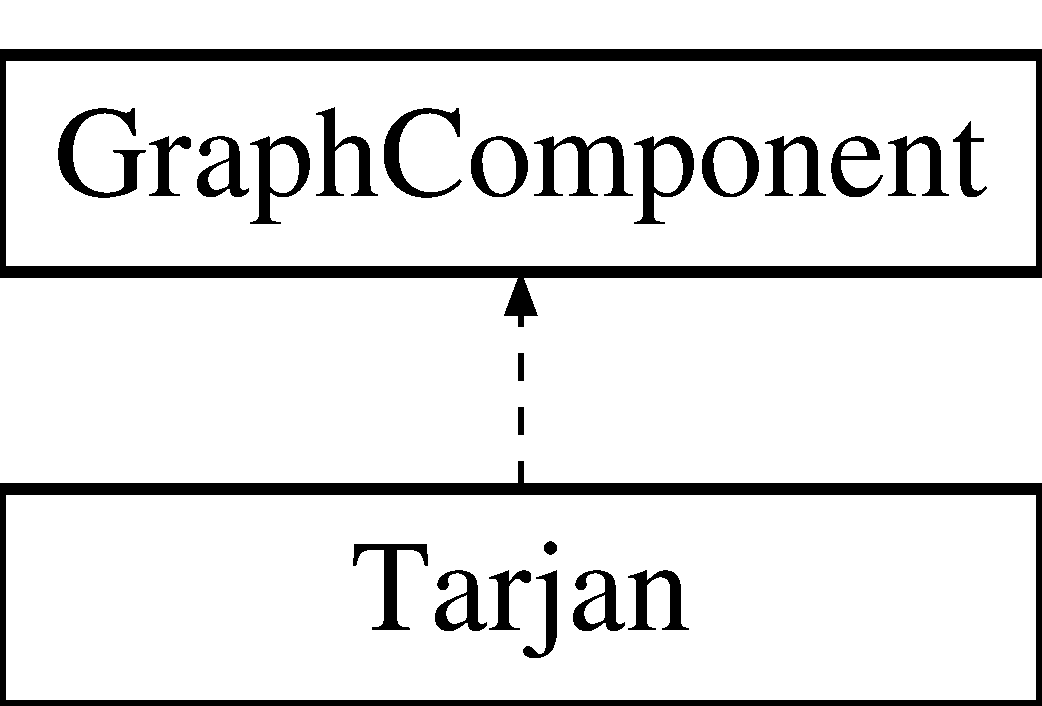
\includegraphics[height=2.000000cm]{class_tarjan}
\end{center}
\end{figure}
\subsection*{Public Member Functions}
\begin{DoxyCompactItemize}
\item 
\hyperlink{class_tarjan_a24a7fa59ed2fcff4a520e012e30acb91}{Tarjan} ()
\item 
\hyperlink{class_tarjan_a7e9845c51e1e905df76b267370c6dc00}{Tarjan} (std\+::string filename)
\item 
void \hyperlink{class_tarjan_af94d48b6e78c292bd1aa465d37d89769}{solve} (int graph\+Num)
\item 
void \hyperlink{class_tarjan_a0ef20e22407703c87c880898c8ad5745}{print\+\_\+graph} ()
\item 
void \hyperlink{class_tarjan_a674767d7e49ada6a738ab69187e4836d}{Apply\+D\+FS} ()
\item 
void \hyperlink{class_tarjan_a277c58dc6f712a6ae1ef2e59c9ad58e1}{Depth\+First\+Search} (\hyperlink{class_graph_component_ae67114a6ce5a001dc35e1996e1b45aa0}{Vertex\+\_\+t} \&v, int \&Counter, std\+::vector$<$ int $>$ \&visited)
\item 
bool \hyperlink{class_tarjan_a74f69dfaa1d4cf3bac06aef7a704c0b8}{is\+Reachable} (\hyperlink{class_graph_component_ae67114a6ce5a001dc35e1996e1b45aa0}{Vertex\+\_\+t} \&source, \hyperlink{class_graph_component_ae67114a6ce5a001dc35e1996e1b45aa0}{Vertex\+\_\+t} \&target)
\item 
\hyperlink{struct_utility_structs_1_1_storage_items}{Utility\+Structs\+::\+Storage\+Items} \hyperlink{class_tarjan_a4be3dec188e347b54a90cd5f37abc268}{apply\+Biconnectivity} ()
\item 
void \hyperlink{class_tarjan_a52573be5a4930ad84f3807bc49f42026}{biconnect} (\hyperlink{class_graph_component_ae67114a6ce5a001dc35e1996e1b45aa0}{Vertex\+\_\+t} \&v, std\+::vector$<$ \hyperlink{utilities_8h_af4a84c740ebb77e6a13a00aa289b0018}{Edge\+\_\+t} $>$ \&edges, int \&Counter, std\+::vector$<$ std\+::vector$<$ \hyperlink{utilities_8h_af4a84c740ebb77e6a13a00aa289b0018}{Edge\+\_\+t} $>$ $>$ \&components, std\+::vector$<$ int $>$ \&visited, std\+::vector$<$ int $>$ \&low\+Pt, int \&stack\+Count)
\item 
\hyperlink{struct_utility_structs_1_1_storage_items}{Utility\+Structs\+::\+Storage\+Items} \hyperlink{class_tarjan_a58ad9fcfd599a608fa1671e4607db378}{Apply\+S\+CC} (bool debug\+Mode)
\item 
void \hyperlink{class_tarjan_ac76fd1419a2de2dbf34c6ff1d4cc55e2}{Strong\+Connect} (\hyperlink{class_graph_component_ae67114a6ce5a001dc35e1996e1b45aa0}{Vertex\+\_\+t} \&v, std\+::vector$<$ \hyperlink{class_graph_component_ae67114a6ce5a001dc35e1996e1b45aa0}{Vertex\+\_\+t} $>$ \&Points, int \&Counter, std\+::vector$<$ int $>$ \&visited, std\+::vector$<$ int $>$ \&low\+Pt, std\+::vector$<$ int $>$ \&low\+Vine, int \&stack\+Count, bool debug\+Mode)
\end{DoxyCompactItemize}
\subsection*{Public Attributes}
\begin{DoxyCompactItemize}
\item 
\hyperlink{class_graph_component_a982e0748a6e1b8dc74986f5f8b3dca5c}{the\+Graph} \hyperlink{class_tarjan_a54b0703f885a3514ea0bf4cdbc7fdaad}{t}
\item 
std\+::vector$<$ \hyperlink{class_graph_component_a982e0748a6e1b8dc74986f5f8b3dca5c}{the\+Graph} $>$ \hyperlink{class_tarjan_aaa327f105a07f07648dcc6f62a565986}{experiment}
\end{DoxyCompactItemize}
\subsection*{Additional Inherited Members}


\subsection{Detailed Description}
This class contains the implementation of algorithms from the \hyperlink{class_tarjan}{Tarjan}\textquotesingle{}s paper. 

\subsection{Constructor \& Destructor Documentation}
\mbox{\Hypertarget{class_tarjan_a24a7fa59ed2fcff4a520e012e30acb91}\label{class_tarjan_a24a7fa59ed2fcff4a520e012e30acb91}} 
\index{Tarjan@{Tarjan}!Tarjan@{Tarjan}}
\index{Tarjan@{Tarjan}!Tarjan@{Tarjan}}
\subsubsection{\texorpdfstring{Tarjan()}{Tarjan()}\hspace{0.1cm}{\footnotesize\ttfamily [1/2]}}
{\footnotesize\ttfamily Tarjan\+::\+Tarjan (\begin{DoxyParamCaption}{ }\end{DoxyParamCaption})\hspace{0.3cm}{\ttfamily [inline]}}

\mbox{\Hypertarget{class_tarjan_a7e9845c51e1e905df76b267370c6dc00}\label{class_tarjan_a7e9845c51e1e905df76b267370c6dc00}} 
\index{Tarjan@{Tarjan}!Tarjan@{Tarjan}}
\index{Tarjan@{Tarjan}!Tarjan@{Tarjan}}
\subsubsection{\texorpdfstring{Tarjan()}{Tarjan()}\hspace{0.1cm}{\footnotesize\ttfamily [2/2]}}
{\footnotesize\ttfamily Tarjan\+::\+Tarjan (\begin{DoxyParamCaption}\item[{std\+::string}]{filename }\end{DoxyParamCaption})\hspace{0.3cm}{\ttfamily [inline]}}



\subsection{Member Function Documentation}
\mbox{\Hypertarget{class_tarjan_a4be3dec188e347b54a90cd5f37abc268}\label{class_tarjan_a4be3dec188e347b54a90cd5f37abc268}} 
\index{Tarjan@{Tarjan}!apply\+Biconnectivity@{apply\+Biconnectivity}}
\index{apply\+Biconnectivity@{apply\+Biconnectivity}!Tarjan@{Tarjan}}
\subsubsection{\texorpdfstring{apply\+Biconnectivity()}{applyBiconnectivity()}}
{\footnotesize\ttfamily \hyperlink{struct_utility_structs_1_1_storage_items}{Utility\+Structs\+::\+Storage\+Items} Tarjan\+::apply\+Biconnectivity (\begin{DoxyParamCaption}{ }\end{DoxyParamCaption})}

\mbox{\Hypertarget{class_tarjan_a674767d7e49ada6a738ab69187e4836d}\label{class_tarjan_a674767d7e49ada6a738ab69187e4836d}} 
\index{Tarjan@{Tarjan}!Apply\+D\+FS@{Apply\+D\+FS}}
\index{Apply\+D\+FS@{Apply\+D\+FS}!Tarjan@{Tarjan}}
\subsubsection{\texorpdfstring{Apply\+D\+F\+S()}{ApplyDFS()}}
{\footnotesize\ttfamily void Tarjan\+::\+Apply\+D\+FS (\begin{DoxyParamCaption}{ }\end{DoxyParamCaption})}

\mbox{\Hypertarget{class_tarjan_a58ad9fcfd599a608fa1671e4607db378}\label{class_tarjan_a58ad9fcfd599a608fa1671e4607db378}} 
\index{Tarjan@{Tarjan}!Apply\+S\+CC@{Apply\+S\+CC}}
\index{Apply\+S\+CC@{Apply\+S\+CC}!Tarjan@{Tarjan}}
\subsubsection{\texorpdfstring{Apply\+S\+C\+C()}{ApplySCC()}}
{\footnotesize\ttfamily \hyperlink{struct_utility_structs_1_1_storage_items}{Utility\+Structs\+::\+Storage\+Items} Tarjan\+::\+Apply\+S\+CC (\begin{DoxyParamCaption}\item[{bool}]{debug\+Mode }\end{DoxyParamCaption})}

\mbox{\Hypertarget{class_tarjan_a52573be5a4930ad84f3807bc49f42026}\label{class_tarjan_a52573be5a4930ad84f3807bc49f42026}} 
\index{Tarjan@{Tarjan}!biconnect@{biconnect}}
\index{biconnect@{biconnect}!Tarjan@{Tarjan}}
\subsubsection{\texorpdfstring{biconnect()}{biconnect()}}
{\footnotesize\ttfamily void Tarjan\+::biconnect (\begin{DoxyParamCaption}\item[{\hyperlink{class_graph_component_ae67114a6ce5a001dc35e1996e1b45aa0}{Vertex\+\_\+t} \&}]{v,  }\item[{std\+::vector$<$ \hyperlink{utilities_8h_af4a84c740ebb77e6a13a00aa289b0018}{Edge\+\_\+t} $>$ \&}]{edges,  }\item[{int \&}]{Counter,  }\item[{std\+::vector$<$ std\+::vector$<$ \hyperlink{utilities_8h_af4a84c740ebb77e6a13a00aa289b0018}{Edge\+\_\+t} $>$ $>$ \&}]{components,  }\item[{std\+::vector$<$ int $>$ \&}]{visited,  }\item[{std\+::vector$<$ int $>$ \&}]{low\+Pt,  }\item[{int \&}]{stack\+Count }\end{DoxyParamCaption})}

\mbox{\Hypertarget{class_tarjan_a277c58dc6f712a6ae1ef2e59c9ad58e1}\label{class_tarjan_a277c58dc6f712a6ae1ef2e59c9ad58e1}} 
\index{Tarjan@{Tarjan}!Depth\+First\+Search@{Depth\+First\+Search}}
\index{Depth\+First\+Search@{Depth\+First\+Search}!Tarjan@{Tarjan}}
\subsubsection{\texorpdfstring{Depth\+First\+Search()}{DepthFirstSearch()}}
{\footnotesize\ttfamily void Tarjan\+::\+Depth\+First\+Search (\begin{DoxyParamCaption}\item[{\hyperlink{class_graph_component_ae67114a6ce5a001dc35e1996e1b45aa0}{Vertex\+\_\+t} \&}]{v,  }\item[{int \&}]{Counter,  }\item[{std\+::vector$<$ int $>$ \&}]{visited }\end{DoxyParamCaption})}

\mbox{\Hypertarget{class_tarjan_a74f69dfaa1d4cf3bac06aef7a704c0b8}\label{class_tarjan_a74f69dfaa1d4cf3bac06aef7a704c0b8}} 
\index{Tarjan@{Tarjan}!is\+Reachable@{is\+Reachable}}
\index{is\+Reachable@{is\+Reachable}!Tarjan@{Tarjan}}
\subsubsection{\texorpdfstring{is\+Reachable()}{isReachable()}}
{\footnotesize\ttfamily bool Tarjan\+::is\+Reachable (\begin{DoxyParamCaption}\item[{\hyperlink{class_graph_component_ae67114a6ce5a001dc35e1996e1b45aa0}{Vertex\+\_\+t} \&}]{source,  }\item[{\hyperlink{class_graph_component_ae67114a6ce5a001dc35e1996e1b45aa0}{Vertex\+\_\+t} \&}]{target }\end{DoxyParamCaption})}

\mbox{\Hypertarget{class_tarjan_a0ef20e22407703c87c880898c8ad5745}\label{class_tarjan_a0ef20e22407703c87c880898c8ad5745}} 
\index{Tarjan@{Tarjan}!print\+\_\+graph@{print\+\_\+graph}}
\index{print\+\_\+graph@{print\+\_\+graph}!Tarjan@{Tarjan}}
\subsubsection{\texorpdfstring{print\+\_\+graph()}{print\_graph()}}
{\footnotesize\ttfamily void Tarjan\+::print\+\_\+graph (\begin{DoxyParamCaption}{ }\end{DoxyParamCaption})}

\mbox{\Hypertarget{class_tarjan_af94d48b6e78c292bd1aa465d37d89769}\label{class_tarjan_af94d48b6e78c292bd1aa465d37d89769}} 
\index{Tarjan@{Tarjan}!solve@{solve}}
\index{solve@{solve}!Tarjan@{Tarjan}}
\subsubsection{\texorpdfstring{solve()}{solve()}}
{\footnotesize\ttfamily void Tarjan\+::solve (\begin{DoxyParamCaption}\item[{int}]{graph\+Num }\end{DoxyParamCaption})}

\mbox{\Hypertarget{class_tarjan_ac76fd1419a2de2dbf34c6ff1d4cc55e2}\label{class_tarjan_ac76fd1419a2de2dbf34c6ff1d4cc55e2}} 
\index{Tarjan@{Tarjan}!Strong\+Connect@{Strong\+Connect}}
\index{Strong\+Connect@{Strong\+Connect}!Tarjan@{Tarjan}}
\subsubsection{\texorpdfstring{Strong\+Connect()}{StrongConnect()}}
{\footnotesize\ttfamily void Tarjan\+::\+Strong\+Connect (\begin{DoxyParamCaption}\item[{\hyperlink{class_graph_component_ae67114a6ce5a001dc35e1996e1b45aa0}{Vertex\+\_\+t} \&}]{v,  }\item[{std\+::vector$<$ \hyperlink{class_graph_component_ae67114a6ce5a001dc35e1996e1b45aa0}{Vertex\+\_\+t} $>$ \&}]{Points,  }\item[{int \&}]{Counter,  }\item[{std\+::vector$<$ int $>$ \&}]{visited,  }\item[{std\+::vector$<$ int $>$ \&}]{low\+Pt,  }\item[{std\+::vector$<$ int $>$ \&}]{low\+Vine,  }\item[{int \&}]{stack\+Count,  }\item[{bool}]{debug\+Mode }\end{DoxyParamCaption})}



\subsection{Member Data Documentation}
\mbox{\Hypertarget{class_tarjan_aaa327f105a07f07648dcc6f62a565986}\label{class_tarjan_aaa327f105a07f07648dcc6f62a565986}} 
\index{Tarjan@{Tarjan}!experiment@{experiment}}
\index{experiment@{experiment}!Tarjan@{Tarjan}}
\subsubsection{\texorpdfstring{experiment}{experiment}}
{\footnotesize\ttfamily std\+::vector$<$\hyperlink{class_graph_component_a982e0748a6e1b8dc74986f5f8b3dca5c}{the\+Graph}$>$ Tarjan\+::experiment}

\mbox{\Hypertarget{class_tarjan_a54b0703f885a3514ea0bf4cdbc7fdaad}\label{class_tarjan_a54b0703f885a3514ea0bf4cdbc7fdaad}} 
\index{Tarjan@{Tarjan}!t@{t}}
\index{t@{t}!Tarjan@{Tarjan}}
\subsubsection{\texorpdfstring{t}{t}}
{\footnotesize\ttfamily \hyperlink{class_graph_component_a982e0748a6e1b8dc74986f5f8b3dca5c}{the\+Graph} Tarjan\+::t}



The documentation for this class was generated from the following file\+:\begin{DoxyCompactItemize}
\item 
header/\hyperlink{tarjan_8h}{tarjan.\+h}\end{DoxyCompactItemize}

\hypertarget{class_utility_structs_1_1_timer}{}\section{Utility\+Structs\+:\+:Timer Class Reference}
\label{class_utility_structs_1_1_timer}\index{Utility\+Structs\+::\+Timer@{Utility\+Structs\+::\+Timer}}


This class is used to measure the execution time of a executed function with the same scope.  




{\ttfamily \#include $<$utilities.\+h$>$}

\subsection*{Public Member Functions}
\begin{DoxyCompactItemize}
\item 
\hyperlink{class_utility_structs_1_1_timer_a8513b72cae3808920cc5f76c28b34d63}{Timer} ()
\item 
float \hyperlink{class_utility_structs_1_1_timer_a12f62b57c263d563efd6089cff52355f}{stop} ()
\item 
\hyperlink{class_utility_structs_1_1_timer_a377c1febadb76e78d9a36bd81b3ab676}{$\sim$\+Timer} ()
\end{DoxyCompactItemize}
\subsection*{Public Attributes}
\begin{DoxyCompactItemize}
\item 
std\+::chrono\+::time\+\_\+point$<$ std\+::chrono\+::steady\+\_\+clock $>$ \hyperlink{class_utility_structs_1_1_timer_a60bc754cb86990dad0003e8d49048c07}{start}
\item 
std\+::chrono\+::duration$<$ float $>$ \hyperlink{class_utility_structs_1_1_timer_aa78ff6477de7008371025bd459a262e4}{duration}
\item 
std\+::chrono\+::time\+\_\+point$<$ std\+::chrono\+::steady\+\_\+clock $>$ \hyperlink{class_utility_structs_1_1_timer_a9b87226726489b3885d6faf4373c34b5}{finish}
\end{DoxyCompactItemize}


\subsection{Detailed Description}
This class is used to measure the execution time of a executed function with the same scope. 

Definition at line 64 of file utilities.\+h.



\subsection{Constructor \& Destructor Documentation}
\mbox{\Hypertarget{class_utility_structs_1_1_timer_a8513b72cae3808920cc5f76c28b34d63}\label{class_utility_structs_1_1_timer_a8513b72cae3808920cc5f76c28b34d63}} 
\index{Utility\+Structs\+::\+Timer@{Utility\+Structs\+::\+Timer}!Timer@{Timer}}
\index{Timer@{Timer}!Utility\+Structs\+::\+Timer@{Utility\+Structs\+::\+Timer}}
\subsubsection{\texorpdfstring{Timer()}{Timer()}}
{\footnotesize\ttfamily Utility\+Structs\+::\+Timer\+::\+Timer (\begin{DoxyParamCaption}{ }\end{DoxyParamCaption})\hspace{0.3cm}{\ttfamily [inline]}}



Definition at line 71 of file utilities.\+h.


\begin{DoxyCode}
72     \{
73         \hyperlink{class_utility_structs_1_1_timer_a60bc754cb86990dad0003e8d49048c07}{start} = std::chrono::high\_resolution\_clock::now();
74     \}
\end{DoxyCode}
\mbox{\Hypertarget{class_utility_structs_1_1_timer_a377c1febadb76e78d9a36bd81b3ab676}\label{class_utility_structs_1_1_timer_a377c1febadb76e78d9a36bd81b3ab676}} 
\index{Utility\+Structs\+::\+Timer@{Utility\+Structs\+::\+Timer}!````~Timer@{$\sim$\+Timer}}
\index{````~Timer@{$\sim$\+Timer}!Utility\+Structs\+::\+Timer@{Utility\+Structs\+::\+Timer}}
\subsubsection{\texorpdfstring{$\sim$\+Timer()}{~Timer()}}
{\footnotesize\ttfamily Utility\+Structs\+::\+Timer\+::$\sim$\+Timer (\begin{DoxyParamCaption}{ }\end{DoxyParamCaption})\hspace{0.3cm}{\ttfamily [inline]}}



Definition at line 83 of file utilities.\+h.


\begin{DoxyCode}
84     \{
85         \hyperlink{class_utility_structs_1_1_timer_a9b87226726489b3885d6faf4373c34b5}{finish} = std::chrono::high\_resolution\_clock::now();
86         \hyperlink{class_utility_structs_1_1_timer_aa78ff6477de7008371025bd459a262e4}{duration} = \hyperlink{class_utility_structs_1_1_timer_a9b87226726489b3885d6faf4373c34b5}{finish} - \hyperlink{class_utility_structs_1_1_timer_a60bc754cb86990dad0003e8d49048c07}{start};
87         \textcolor{keywordtype}{float} ms = \hyperlink{class_utility_structs_1_1_timer_aa78ff6477de7008371025bd459a262e4}{duration}.count() * 1000.000f;
88     \}
\end{DoxyCode}


\subsection{Member Function Documentation}
\mbox{\Hypertarget{class_utility_structs_1_1_timer_a12f62b57c263d563efd6089cff52355f}\label{class_utility_structs_1_1_timer_a12f62b57c263d563efd6089cff52355f}} 
\index{Utility\+Structs\+::\+Timer@{Utility\+Structs\+::\+Timer}!stop@{stop}}
\index{stop@{stop}!Utility\+Structs\+::\+Timer@{Utility\+Structs\+::\+Timer}}
\subsubsection{\texorpdfstring{stop()}{stop()}}
{\footnotesize\ttfamily float Utility\+Structs\+::\+Timer\+::stop (\begin{DoxyParamCaption}{ }\end{DoxyParamCaption})\hspace{0.3cm}{\ttfamily [inline]}}



Definition at line 75 of file utilities.\+h.


\begin{DoxyCode}
76     \{
77         \hyperlink{class_utility_structs_1_1_timer_a9b87226726489b3885d6faf4373c34b5}{finish} = std::chrono::high\_resolution\_clock::now();
78         \hyperlink{class_utility_structs_1_1_timer_aa78ff6477de7008371025bd459a262e4}{duration} = \hyperlink{class_utility_structs_1_1_timer_a9b87226726489b3885d6faf4373c34b5}{finish} - \hyperlink{class_utility_structs_1_1_timer_a60bc754cb86990dad0003e8d49048c07}{start};
79         \textcolor{keywordtype}{float} ms = \hyperlink{class_utility_structs_1_1_timer_aa78ff6477de7008371025bd459a262e4}{duration}.count() * 1000.0f;
80 
81         \textcolor{keywordflow}{return} ms;
82     \}
\end{DoxyCode}


\subsection{Member Data Documentation}
\mbox{\Hypertarget{class_utility_structs_1_1_timer_aa78ff6477de7008371025bd459a262e4}\label{class_utility_structs_1_1_timer_aa78ff6477de7008371025bd459a262e4}} 
\index{Utility\+Structs\+::\+Timer@{Utility\+Structs\+::\+Timer}!duration@{duration}}
\index{duration@{duration}!Utility\+Structs\+::\+Timer@{Utility\+Structs\+::\+Timer}}
\subsubsection{\texorpdfstring{duration}{duration}}
{\footnotesize\ttfamily std\+::chrono\+::duration$<$float$>$ Utility\+Structs\+::\+Timer\+::duration}



Definition at line 68 of file utilities.\+h.

\mbox{\Hypertarget{class_utility_structs_1_1_timer_a9b87226726489b3885d6faf4373c34b5}\label{class_utility_structs_1_1_timer_a9b87226726489b3885d6faf4373c34b5}} 
\index{Utility\+Structs\+::\+Timer@{Utility\+Structs\+::\+Timer}!finish@{finish}}
\index{finish@{finish}!Utility\+Structs\+::\+Timer@{Utility\+Structs\+::\+Timer}}
\subsubsection{\texorpdfstring{finish}{finish}}
{\footnotesize\ttfamily std\+::chrono\+::time\+\_\+point$<$std\+::chrono\+::steady\+\_\+clock$>$ Utility\+Structs\+::\+Timer\+::finish}



Definition at line 69 of file utilities.\+h.

\mbox{\Hypertarget{class_utility_structs_1_1_timer_a60bc754cb86990dad0003e8d49048c07}\label{class_utility_structs_1_1_timer_a60bc754cb86990dad0003e8d49048c07}} 
\index{Utility\+Structs\+::\+Timer@{Utility\+Structs\+::\+Timer}!start@{start}}
\index{start@{start}!Utility\+Structs\+::\+Timer@{Utility\+Structs\+::\+Timer}}
\subsubsection{\texorpdfstring{start}{start}}
{\footnotesize\ttfamily std\+::chrono\+::time\+\_\+point$<$std\+::chrono\+::steady\+\_\+clock$>$ Utility\+Structs\+::\+Timer\+::start}



Definition at line 67 of file utilities.\+h.



The documentation for this class was generated from the following file\+:\begin{DoxyCompactItemize}
\item 
header/\hyperlink{utilities_8h}{utilities.\+h}\end{DoxyCompactItemize}

\hypertarget{struct_utility_structs_1_1_vertex_property}{}\section{Utility\+Structs\+:\+:Vertex\+Property Struct Reference}
\label{struct_utility_structs_1_1_vertex_property}\index{Utility\+Structs\+::\+Vertex\+Property@{Utility\+Structs\+::\+Vertex\+Property}}


This struct contains the vertex index info that are used by all of the algorithms.  




{\ttfamily \#include $<$utilities.\+h$>$}

\subsection*{Public Attributes}
\begin{DoxyCompactItemize}
\item 
std\+::size\+\_\+t \hyperlink{struct_utility_structs_1_1_vertex_property_a636cb729438e999aa3d9a17ac39d8641}{index}
\end{DoxyCompactItemize}


\subsection{Detailed Description}
This struct contains the vertex index info that are used by all of the algorithms. 

Definition at line 44 of file utilities.\+h.



\subsection{Member Data Documentation}
\mbox{\Hypertarget{struct_utility_structs_1_1_vertex_property_a636cb729438e999aa3d9a17ac39d8641}\label{struct_utility_structs_1_1_vertex_property_a636cb729438e999aa3d9a17ac39d8641}} 
\index{Utility\+Structs\+::\+Vertex\+Property@{Utility\+Structs\+::\+Vertex\+Property}!index@{index}}
\index{index@{index}!Utility\+Structs\+::\+Vertex\+Property@{Utility\+Structs\+::\+Vertex\+Property}}
\subsubsection{\texorpdfstring{index}{index}}
{\footnotesize\ttfamily std\+::size\+\_\+t Utility\+Structs\+::\+Vertex\+Property\+::index}



Definition at line 46 of file utilities.\+h.



The documentation for this struct was generated from the following file\+:\begin{DoxyCompactItemize}
\item 
header/\hyperlink{utilities_8h}{utilities.\+h}\end{DoxyCompactItemize}

\hypertarget{class_visualize}{}\section{Visualize Class Reference}
\label{class_visualize}\index{Visualize@{Visualize}}


This class is used to visualize the information that are gathered from the algorithms.  




{\ttfamily \#include $<$visualize.\+h$>$}

\subsection*{Public Member Functions}
\begin{DoxyCompactItemize}
\item 
\hyperlink{class_visualize_a8d4163ad53518ec0c8a3eaec2bf2fe7b}{Visualize} ()
\item 
std\+::string \hyperlink{class_visualize_a9d34d81d684587b8b2b8bf70031f1670}{centered} (int \hyperlink{class_visualize_af5ac723ad5f8fe8c4a8378bf1299cda7}{width}, const std\+::string \&str)
\item 
void \hyperlink{class_visualize_a29f27ff8c5e59163eea2be42ff372405}{print\+Program\+Entry} (\hyperlink{struct_session}{Session} \&s)
\item 
void \hyperlink{class_visualize_a3e1aa31f14abdf3cf53662cddc536c6a}{print\+Table\+Banner} ()
\item 
void \hyperlink{class_visualize_a2d38641cb335d7bbf7e11567b07e2d85}{print\+Table\+Seperator} ()
\item 
void \hyperlink{class_visualize_ac0be9ece2d80a7d1e34724fb87424216}{print\+Program\+Bottom} ()
\item 
void \hyperlink{class_visualize_abce6cd538dc0715b21851e0bf0377d85}{print\+Line} (std\+::string message)
\item 
void \hyperlink{class_visualize_a52a0dfaf625bd3ac294a00e3161094cf}{print\+Experiment\+Row} (int id, int vertex, int edge, std\+::vector$<$ \hyperlink{struct_utility_structs_1_1_storage_items}{Utility\+Structs\+::\+Storage\+Items} $>$ row\+Info)
\item 
void \hyperlink{class_visualize_a6e27b451c2662681cb3119e9ff1c22da}{write\+Program\+Entry} (std\+::string filename)
\item 
void \hyperlink{class_visualize_a14c9e9721eeaca0afde25da0138b43b8}{write\+Table\+Banner} (std\+::string filename)
\item 
void \hyperlink{class_visualize_ac5530b8e917c748163e621cf5677eeb5}{write\+Table\+Seperator} (std\+::string filename)
\item 
void \hyperlink{class_visualize_a9ccde29aab876a829335775898373e96}{write\+Line} (std\+::string message, std\+::string filename)
\item 
void \hyperlink{class_visualize_a8aefacec622221533485db6701d1119e}{write\+Experiment\+Row} (int id, int vertex, int edge, std\+::vector$<$ \hyperlink{struct_utility_structs_1_1_storage_items}{Utility\+Structs\+::\+Storage\+Items} $>$ row\+Info, std\+::string filename)
\item 
void \hyperlink{class_visualize_a8677a063c82af1b37b94c7d3a3ca3746}{write\+Experiment\+Row\+\_\+\+C\+SV} (int id, int vertex, int edge, std\+::vector$<$ \hyperlink{struct_utility_structs_1_1_storage_items}{Utility\+Structs\+::\+Storage\+Items} $>$ row\+Info, std\+::string filename)
\end{DoxyCompactItemize}
\subsection*{Public Attributes}
\begin{DoxyCompactItemize}
\item 
int \hyperlink{class_visualize_af5ac723ad5f8fe8c4a8378bf1299cda7}{width}
\end{DoxyCompactItemize}


\subsection{Detailed Description}
This class is used to visualize the information that are gathered from the algorithms. 

\subsection{Constructor \& Destructor Documentation}
\mbox{\Hypertarget{class_visualize_a8d4163ad53518ec0c8a3eaec2bf2fe7b}\label{class_visualize_a8d4163ad53518ec0c8a3eaec2bf2fe7b}} 
\index{Visualize@{Visualize}!Visualize@{Visualize}}
\index{Visualize@{Visualize}!Visualize@{Visualize}}
\subsubsection{\texorpdfstring{Visualize()}{Visualize()}}
{\footnotesize\ttfamily Visualize\+::\+Visualize (\begin{DoxyParamCaption}{ }\end{DoxyParamCaption})\hspace{0.3cm}{\ttfamily [inline]}}



\subsection{Member Function Documentation}
\mbox{\Hypertarget{class_visualize_a9d34d81d684587b8b2b8bf70031f1670}\label{class_visualize_a9d34d81d684587b8b2b8bf70031f1670}} 
\index{Visualize@{Visualize}!centered@{centered}}
\index{centered@{centered}!Visualize@{Visualize}}
\subsubsection{\texorpdfstring{centered()}{centered()}}
{\footnotesize\ttfamily std\+::string Visualize\+::centered (\begin{DoxyParamCaption}\item[{int}]{width,  }\item[{const std\+::string \&}]{str }\end{DoxyParamCaption})}

\mbox{\Hypertarget{class_visualize_a52a0dfaf625bd3ac294a00e3161094cf}\label{class_visualize_a52a0dfaf625bd3ac294a00e3161094cf}} 
\index{Visualize@{Visualize}!print\+Experiment\+Row@{print\+Experiment\+Row}}
\index{print\+Experiment\+Row@{print\+Experiment\+Row}!Visualize@{Visualize}}
\subsubsection{\texorpdfstring{print\+Experiment\+Row()}{printExperimentRow()}}
{\footnotesize\ttfamily void Visualize\+::print\+Experiment\+Row (\begin{DoxyParamCaption}\item[{int}]{id,  }\item[{int}]{vertex,  }\item[{int}]{edge,  }\item[{std\+::vector$<$ \hyperlink{struct_utility_structs_1_1_storage_items}{Utility\+Structs\+::\+Storage\+Items} $>$}]{row\+Info }\end{DoxyParamCaption})}

\mbox{\Hypertarget{class_visualize_abce6cd538dc0715b21851e0bf0377d85}\label{class_visualize_abce6cd538dc0715b21851e0bf0377d85}} 
\index{Visualize@{Visualize}!print\+Line@{print\+Line}}
\index{print\+Line@{print\+Line}!Visualize@{Visualize}}
\subsubsection{\texorpdfstring{print\+Line()}{printLine()}}
{\footnotesize\ttfamily void Visualize\+::print\+Line (\begin{DoxyParamCaption}\item[{std\+::string}]{message }\end{DoxyParamCaption})}

\mbox{\Hypertarget{class_visualize_ac0be9ece2d80a7d1e34724fb87424216}\label{class_visualize_ac0be9ece2d80a7d1e34724fb87424216}} 
\index{Visualize@{Visualize}!print\+Program\+Bottom@{print\+Program\+Bottom}}
\index{print\+Program\+Bottom@{print\+Program\+Bottom}!Visualize@{Visualize}}
\subsubsection{\texorpdfstring{print\+Program\+Bottom()}{printProgramBottom()}}
{\footnotesize\ttfamily void Visualize\+::print\+Program\+Bottom (\begin{DoxyParamCaption}{ }\end{DoxyParamCaption})}

\mbox{\Hypertarget{class_visualize_a29f27ff8c5e59163eea2be42ff372405}\label{class_visualize_a29f27ff8c5e59163eea2be42ff372405}} 
\index{Visualize@{Visualize}!print\+Program\+Entry@{print\+Program\+Entry}}
\index{print\+Program\+Entry@{print\+Program\+Entry}!Visualize@{Visualize}}
\subsubsection{\texorpdfstring{print\+Program\+Entry()}{printProgramEntry()}}
{\footnotesize\ttfamily void Visualize\+::print\+Program\+Entry (\begin{DoxyParamCaption}\item[{\hyperlink{struct_session}{Session} \&}]{s }\end{DoxyParamCaption})}

\mbox{\Hypertarget{class_visualize_a3e1aa31f14abdf3cf53662cddc536c6a}\label{class_visualize_a3e1aa31f14abdf3cf53662cddc536c6a}} 
\index{Visualize@{Visualize}!print\+Table\+Banner@{print\+Table\+Banner}}
\index{print\+Table\+Banner@{print\+Table\+Banner}!Visualize@{Visualize}}
\subsubsection{\texorpdfstring{print\+Table\+Banner()}{printTableBanner()}}
{\footnotesize\ttfamily void Visualize\+::print\+Table\+Banner (\begin{DoxyParamCaption}{ }\end{DoxyParamCaption})}

\mbox{\Hypertarget{class_visualize_a2d38641cb335d7bbf7e11567b07e2d85}\label{class_visualize_a2d38641cb335d7bbf7e11567b07e2d85}} 
\index{Visualize@{Visualize}!print\+Table\+Seperator@{print\+Table\+Seperator}}
\index{print\+Table\+Seperator@{print\+Table\+Seperator}!Visualize@{Visualize}}
\subsubsection{\texorpdfstring{print\+Table\+Seperator()}{printTableSeperator()}}
{\footnotesize\ttfamily void Visualize\+::print\+Table\+Seperator (\begin{DoxyParamCaption}{ }\end{DoxyParamCaption})}

\mbox{\Hypertarget{class_visualize_a8aefacec622221533485db6701d1119e}\label{class_visualize_a8aefacec622221533485db6701d1119e}} 
\index{Visualize@{Visualize}!write\+Experiment\+Row@{write\+Experiment\+Row}}
\index{write\+Experiment\+Row@{write\+Experiment\+Row}!Visualize@{Visualize}}
\subsubsection{\texorpdfstring{write\+Experiment\+Row()}{writeExperimentRow()}}
{\footnotesize\ttfamily void Visualize\+::write\+Experiment\+Row (\begin{DoxyParamCaption}\item[{int}]{id,  }\item[{int}]{vertex,  }\item[{int}]{edge,  }\item[{std\+::vector$<$ \hyperlink{struct_utility_structs_1_1_storage_items}{Utility\+Structs\+::\+Storage\+Items} $>$}]{row\+Info,  }\item[{std\+::string}]{filename }\end{DoxyParamCaption})}

\mbox{\Hypertarget{class_visualize_a8677a063c82af1b37b94c7d3a3ca3746}\label{class_visualize_a8677a063c82af1b37b94c7d3a3ca3746}} 
\index{Visualize@{Visualize}!write\+Experiment\+Row\+\_\+\+C\+SV@{write\+Experiment\+Row\+\_\+\+C\+SV}}
\index{write\+Experiment\+Row\+\_\+\+C\+SV@{write\+Experiment\+Row\+\_\+\+C\+SV}!Visualize@{Visualize}}
\subsubsection{\texorpdfstring{write\+Experiment\+Row\+\_\+\+C\+S\+V()}{writeExperimentRow\_CSV()}}
{\footnotesize\ttfamily void Visualize\+::write\+Experiment\+Row\+\_\+\+C\+SV (\begin{DoxyParamCaption}\item[{int}]{id,  }\item[{int}]{vertex,  }\item[{int}]{edge,  }\item[{std\+::vector$<$ \hyperlink{struct_utility_structs_1_1_storage_items}{Utility\+Structs\+::\+Storage\+Items} $>$}]{row\+Info,  }\item[{std\+::string}]{filename }\end{DoxyParamCaption})}

\mbox{\Hypertarget{class_visualize_a9ccde29aab876a829335775898373e96}\label{class_visualize_a9ccde29aab876a829335775898373e96}} 
\index{Visualize@{Visualize}!write\+Line@{write\+Line}}
\index{write\+Line@{write\+Line}!Visualize@{Visualize}}
\subsubsection{\texorpdfstring{write\+Line()}{writeLine()}}
{\footnotesize\ttfamily void Visualize\+::write\+Line (\begin{DoxyParamCaption}\item[{std\+::string}]{message,  }\item[{std\+::string}]{filename }\end{DoxyParamCaption})}

\mbox{\Hypertarget{class_visualize_a6e27b451c2662681cb3119e9ff1c22da}\label{class_visualize_a6e27b451c2662681cb3119e9ff1c22da}} 
\index{Visualize@{Visualize}!write\+Program\+Entry@{write\+Program\+Entry}}
\index{write\+Program\+Entry@{write\+Program\+Entry}!Visualize@{Visualize}}
\subsubsection{\texorpdfstring{write\+Program\+Entry()}{writeProgramEntry()}}
{\footnotesize\ttfamily void Visualize\+::write\+Program\+Entry (\begin{DoxyParamCaption}\item[{std\+::string}]{filename }\end{DoxyParamCaption})}

\mbox{\Hypertarget{class_visualize_a14c9e9721eeaca0afde25da0138b43b8}\label{class_visualize_a14c9e9721eeaca0afde25da0138b43b8}} 
\index{Visualize@{Visualize}!write\+Table\+Banner@{write\+Table\+Banner}}
\index{write\+Table\+Banner@{write\+Table\+Banner}!Visualize@{Visualize}}
\subsubsection{\texorpdfstring{write\+Table\+Banner()}{writeTableBanner()}}
{\footnotesize\ttfamily void Visualize\+::write\+Table\+Banner (\begin{DoxyParamCaption}\item[{std\+::string}]{filename }\end{DoxyParamCaption})}

\mbox{\Hypertarget{class_visualize_ac5530b8e917c748163e621cf5677eeb5}\label{class_visualize_ac5530b8e917c748163e621cf5677eeb5}} 
\index{Visualize@{Visualize}!write\+Table\+Seperator@{write\+Table\+Seperator}}
\index{write\+Table\+Seperator@{write\+Table\+Seperator}!Visualize@{Visualize}}
\subsubsection{\texorpdfstring{write\+Table\+Seperator()}{writeTableSeperator()}}
{\footnotesize\ttfamily void Visualize\+::write\+Table\+Seperator (\begin{DoxyParamCaption}\item[{std\+::string}]{filename }\end{DoxyParamCaption})}



\subsection{Member Data Documentation}
\mbox{\Hypertarget{class_visualize_af5ac723ad5f8fe8c4a8378bf1299cda7}\label{class_visualize_af5ac723ad5f8fe8c4a8378bf1299cda7}} 
\index{Visualize@{Visualize}!width@{width}}
\index{width@{width}!Visualize@{Visualize}}
\subsubsection{\texorpdfstring{width}{width}}
{\footnotesize\ttfamily int Visualize\+::width}



The documentation for this class was generated from the following file\+:\begin{DoxyCompactItemize}
\item 
header/\hyperlink{visualize_8h}{visualize.\+h}\end{DoxyCompactItemize}

\chapter{File Documentation}
\hypertarget{analyzer_8h}{}\section{header/analyzer.h File Reference}
\label{analyzer_8h}\index{header/analyzer.\+h@{header/analyzer.\+h}}
{\ttfamily \#include \char`\"{}./graphcomponent.\+h\char`\"{}}\newline
{\ttfamily \#include \char`\"{}./visualize.\+h\char`\"{}}\newline
{\ttfamily \#include $<$iostream$>$}\newline
{\ttfamily \#include $<$vector$>$}\newline
{\ttfamily \#include $<$string$>$}\newline
{\ttfamily \#include $<$fstream$>$}\newline
{\ttfamily \#include $<$sstream$>$}\newline
{\ttfamily \#include $<$iterator$>$}\newline
{\ttfamily \#include $<$chrono$>$}\newline
{\ttfamily \#include $<$thread$>$}\newline
{\ttfamily \#include $<$time.\+h$>$}\newline
{\ttfamily \#include $<$boost/config.\+hpp$>$}\newline
{\ttfamily \#include $<$boost/filesystem.\+hpp$>$}\newline
{\ttfamily \#include $<$boost/graph/adjacency\+\_\+list.\+hpp$>$}\newline
{\ttfamily \#include $<$boost/graph/graphviz.\+hpp$>$}\newline
{\ttfamily \#include $<$boost/graph/graph\+\_\+utility.\+hpp$>$}\newline
{\ttfamily \#include $<$boost/graph/adjacency\+\_\+list\+\_\+io.\+hpp$>$}\newline
{\ttfamily \#include $<$boost/graph/property\+\_\+iter\+\_\+range.\+hpp$>$}\newline
{\ttfamily \#include $<$boost/graph/copy.\+hpp$>$}\newline
{\ttfamily \#include $<$boost/property\+\_\+map/property\+\_\+map.\+hpp$>$}\newline
\subsection*{Classes}
\begin{DoxyCompactItemize}
\item 
class \hyperlink{class_analyzer}{Analyzer}
\begin{DoxyCompactList}\small\item\em This class is mainly responsible for the experiment functionality. It also provides the wrapped experiment methods. \end{DoxyCompactList}\end{DoxyCompactItemize}

\hypertarget{application_8h}{}\section{header/application.h File Reference}
\label{application_8h}\index{header/application.\+h@{header/application.\+h}}
{\ttfamily \#include \char`\"{}./visualize.\+h\char`\"{}}\newline
{\ttfamily \#include \char`\"{}./analyzer.\+h\char`\"{}}\newline
{\ttfamily \#include \char`\"{}./utilities.\+h\char`\"{}}\newline
\subsection*{Classes}
\begin{DoxyCompactItemize}
\item 
class \hyperlink{class_application}{Application}
\end{DoxyCompactItemize}

\hypertarget{graphcomponent_8h}{}\section{header/graphcomponent.h File Reference}
\label{graphcomponent_8h}\index{header/graphcomponent.\+h@{header/graphcomponent.\+h}}
{\ttfamily \#include \char`\"{}utilities.\+h\char`\"{}}\newline
{\ttfamily \#include $<$iostream$>$}\newline
{\ttfamily \#include $<$vector$>$}\newline
{\ttfamily \#include $<$string$>$}\newline
{\ttfamily \#include $<$fstream$>$}\newline
{\ttfamily \#include $<$sstream$>$}\newline
{\ttfamily \#include $<$iterator$>$}\newline
{\ttfamily \#include $<$boost/config.\+hpp$>$}\newline
{\ttfamily \#include $<$boost/graph/adjacency\+\_\+list.\+hpp$>$}\newline
{\ttfamily \#include $<$boost/graph/graphviz.\+hpp$>$}\newline
{\ttfamily \#include $<$boost/graph/graph\+\_\+utility.\+hpp$>$}\newline
{\ttfamily \#include $<$boost/graph/adjacency\+\_\+list\+\_\+io.\+hpp$>$}\newline
{\ttfamily \#include $<$boost/graph/property\+\_\+iter\+\_\+range.\+hpp$>$}\newline
{\ttfamily \#include $<$boost/graph/copy.\+hpp$>$}\newline
{\ttfamily \#include $<$boost/property\+\_\+map/property\+\_\+map.\+hpp$>$}\newline
\subsection*{Classes}
\begin{DoxyCompactItemize}
\item 
class \hyperlink{class_graph_component}{Graph\+Component}
\begin{DoxyCompactList}\small\item\em This class is used to read graphs from the file and import them to the Boost Graph objects. \end{DoxyCompactList}\end{DoxyCompactItemize}

\hypertarget{nuutila_8h}{}\section{header/nuutila.h File Reference}
\label{nuutila_8h}\index{header/nuutila.\+h@{header/nuutila.\+h}}
{\ttfamily \#include \char`\"{}./graphcomponent.\+h\char`\"{}}\newline
{\ttfamily \#include \char`\"{}./analyzer.\+h\char`\"{}}\newline
{\ttfamily \#include $<$iostream$>$}\newline
{\ttfamily \#include $<$vector$>$}\newline
{\ttfamily \#include $<$string$>$}\newline
{\ttfamily \#include $<$fstream$>$}\newline
{\ttfamily \#include $<$sstream$>$}\newline
{\ttfamily \#include $<$iterator$>$}\newline
{\ttfamily \#include $<$boost/config.\+hpp$>$}\newline
{\ttfamily \#include $<$boost/graph/adjacency\+\_\+list.\+hpp$>$}\newline
{\ttfamily \#include $<$boost/graph/graphviz.\+hpp$>$}\newline
{\ttfamily \#include $<$boost/graph/graph\+\_\+utility.\+hpp$>$}\newline
{\ttfamily \#include $<$boost/graph/adjacency\+\_\+list\+\_\+io.\+hpp$>$}\newline
{\ttfamily \#include $<$boost/graph/property\+\_\+iter\+\_\+range.\+hpp$>$}\newline
{\ttfamily \#include $<$boost/graph/copy.\+hpp$>$}\newline
{\ttfamily \#include $<$boost/property\+\_\+map/property\+\_\+map.\+hpp$>$}\newline
\subsection*{Classes}
\begin{DoxyCompactItemize}
\item 
class \hyperlink{class_nuutila}{Nuutila}
\begin{DoxyCompactList}\small\item\em This class contains the implementations of algorithms from the \hyperlink{class_nuutila}{Nuutila}\textquotesingle{}s Paper. \end{DoxyCompactList}\end{DoxyCompactItemize}

\hypertarget{pearce_8h}{}\section{header/pearce.h File Reference}
\label{pearce_8h}\index{header/pearce.\+h@{header/pearce.\+h}}
{\ttfamily \#include \char`\"{}./graphcomponent.\+h\char`\"{}}\newline
{\ttfamily \#include \char`\"{}./analyzer.\+h\char`\"{}}\newline
{\ttfamily \#include $<$iostream$>$}\newline
{\ttfamily \#include $<$vector$>$}\newline
{\ttfamily \#include $<$string$>$}\newline
{\ttfamily \#include $<$fstream$>$}\newline
{\ttfamily \#include $<$sstream$>$}\newline
{\ttfamily \#include $<$iterator$>$}\newline
{\ttfamily \#include $<$boost/config.\+hpp$>$}\newline
{\ttfamily \#include $<$boost/graph/adjacency\+\_\+list.\+hpp$>$}\newline
{\ttfamily \#include $<$boost/graph/graphviz.\+hpp$>$}\newline
{\ttfamily \#include $<$boost/graph/graph\+\_\+utility.\+hpp$>$}\newline
{\ttfamily \#include $<$boost/graph/adjacency\+\_\+list\+\_\+io.\+hpp$>$}\newline
{\ttfamily \#include $<$boost/graph/property\+\_\+iter\+\_\+range.\+hpp$>$}\newline
{\ttfamily \#include $<$boost/graph/copy.\+hpp$>$}\newline
{\ttfamily \#include $<$boost/property\+\_\+map/property\+\_\+map.\+hpp$>$}\newline
\subsection*{Classes}
\begin{DoxyCompactItemize}
\item 
class \hyperlink{class_pearce}{Pearce}
\begin{DoxyCompactList}\small\item\em This class contains the implementation of algorithms from the \hyperlink{class_pearce}{Pearce}\textquotesingle{}s paper. \end{DoxyCompactList}\end{DoxyCompactItemize}

\hypertarget{tarjan_8h}{}\section{header/tarjan.h File Reference}
\label{tarjan_8h}\index{header/tarjan.\+h@{header/tarjan.\+h}}
{\ttfamily \#include \char`\"{}./graphcomponent.\+h\char`\"{}}\newline
{\ttfamily \#include \char`\"{}./analyzer.\+h\char`\"{}}\newline
{\ttfamily \#include $<$iostream$>$}\newline
{\ttfamily \#include $<$vector$>$}\newline
{\ttfamily \#include $<$string$>$}\newline
{\ttfamily \#include $<$fstream$>$}\newline
{\ttfamily \#include $<$sstream$>$}\newline
{\ttfamily \#include $<$iterator$>$}\newline
{\ttfamily \#include $<$boost/config.\+hpp$>$}\newline
{\ttfamily \#include $<$boost/graph/adjacency\+\_\+list.\+hpp$>$}\newline
{\ttfamily \#include $<$boost/graph/graphviz.\+hpp$>$}\newline
{\ttfamily \#include $<$boost/graph/graph\+\_\+utility.\+hpp$>$}\newline
{\ttfamily \#include $<$boost/graph/adjacency\+\_\+list\+\_\+io.\+hpp$>$}\newline
{\ttfamily \#include $<$boost/graph/property\+\_\+iter\+\_\+range.\+hpp$>$}\newline
{\ttfamily \#include $<$boost/graph/copy.\+hpp$>$}\newline
{\ttfamily \#include $<$boost/property\+\_\+map/property\+\_\+map.\+hpp$>$}\newline
\subsection*{Classes}
\begin{DoxyCompactItemize}
\item 
class \hyperlink{class_tarjan}{Tarjan}
\end{DoxyCompactItemize}

\hypertarget{utilities_8h}{}\section{header/utilities.h File Reference}
\label{utilities_8h}\index{header/utilities.\+h@{header/utilities.\+h}}
{\ttfamily \#include $<$boost/config.\+hpp$>$}\newline
{\ttfamily \#include $<$boost/graph/adjacency\+\_\+list.\+hpp$>$}\newline
{\ttfamily \#include $<$boost/graph/graphviz.\+hpp$>$}\newline
{\ttfamily \#include $<$boost/graph/graph\+\_\+utility.\+hpp$>$}\newline
{\ttfamily \#include $<$boost/graph/adjacency\+\_\+list\+\_\+io.\+hpp$>$}\newline
{\ttfamily \#include $<$boost/graph/property\+\_\+iter\+\_\+range.\+hpp$>$}\newline
{\ttfamily \#include $<$boost/graph/copy.\+hpp$>$}\newline
{\ttfamily \#include $<$boost/property\+\_\+map/property\+\_\+map.\+hpp$>$}\newline
{\ttfamily \#include $<$time.\+h$>$}\newline
\subsection*{Classes}
\begin{DoxyCompactItemize}
\item 
struct \hyperlink{struct_session}{Session}
\begin{DoxyCompactList}\small\item\em This struct is used to contain information about the last generated graph directive and the experiment result for users. \end{DoxyCompactList}\item 
struct \hyperlink{struct_utility_structs_1_1_edge_property}{Utility\+Structs\+::\+Edge\+Property}
\begin{DoxyCompactList}\small\item\em This struct contains the edge type info for \hyperlink{class_tarjan}{Tarjan}\textquotesingle{}s S\+CC Algorithm. \end{DoxyCompactList}\item 
struct \hyperlink{struct_utility_structs_1_1_vertex_property}{Utility\+Structs\+::\+Vertex\+Property}
\begin{DoxyCompactList}\small\item\em This struct contains the vertex index info that are used by all of the algorithms. \end{DoxyCompactList}\item 
struct \hyperlink{struct_utility_structs_1_1_storage_items}{Utility\+Structs\+::\+Storage\+Items}
\begin{DoxyCompactList}\small\item\em This struct is used to store all of the output information of algorithms for later use. \end{DoxyCompactList}\item 
class \hyperlink{class_utility_structs_1_1_timer}{Utility\+Structs\+::\+Timer}
\begin{DoxyCompactList}\small\item\em This class is used to measure the execution time of a executed function with the same scope. \end{DoxyCompactList}\end{DoxyCompactItemize}
\subsection*{Namespaces}
\begin{DoxyCompactItemize}
\item 
 \hyperlink{namespace_utility_structs}{Utility\+Structs}
\end{DoxyCompactItemize}
\subsection*{Macros}
\begin{DoxyCompactItemize}
\item 
\#define \hyperlink{utilities_8h_a5ee336838879920d67d1f9c59217dbe0}{P\+R\+O\+G\+R\+A\+M\+\_\+\+W\+I\+D\+TH}~180
\end{DoxyCompactItemize}
\subsection*{Typedefs}
\begin{DoxyCompactItemize}
\item 
typedef \hyperlink{struct_utility_structs_1_1_vertex_property}{Utility\+Structs\+::\+Vertex\+Property} \hyperlink{utilities_8h_a4fda301c7fcca0db1cda24ed568e72a2}{Vertex\+Property}
\item 
typedef \hyperlink{struct_utility_structs_1_1_edge_property}{Utility\+Structs\+::\+Edge\+Property} \hyperlink{utilities_8h_ad3033bfd11bff70cf37c0715a9dd2bd5}{Edge\+Property}
\item 
typedef boost\+::adjacency\+\_\+list$<$ boost\+::vecS, boost\+::listS, boost\+::directedS, \hyperlink{utilities_8h_a4fda301c7fcca0db1cda24ed568e72a2}{Vertex\+Property}, \hyperlink{utilities_8h_ad3033bfd11bff70cf37c0715a9dd2bd5}{Edge\+Property} $>$ \hyperlink{utilities_8h_a0454e560170658194abd1bd3ef03bf70}{the\+Graph}
\item 
typedef boost\+::graph\+\_\+traits$<$ \hyperlink{utilities_8h_a0454e560170658194abd1bd3ef03bf70}{the\+Graph} $>$\+::vertex\+\_\+descriptor \hyperlink{utilities_8h_a344cd987714d06997f0becda3c96d6e2}{Vertex\+\_\+t}
\item 
typedef boost\+::graph\+\_\+traits$<$ \hyperlink{utilities_8h_a0454e560170658194abd1bd3ef03bf70}{the\+Graph} $>$\+::edge\+\_\+descriptor \hyperlink{utilities_8h_af4a84c740ebb77e6a13a00aa289b0018}{Edge\+\_\+t}
\item 
typedef boost\+::graph\+\_\+traits$<$ \hyperlink{utilities_8h_a0454e560170658194abd1bd3ef03bf70}{the\+Graph} $>$\+::edge\+\_\+descriptor \hyperlink{utilities_8h_abc70257bbb251602ecdc30866b83f7de}{Edge}
\item 
typedef property\+\_\+map$<$ \hyperlink{utilities_8h_a0454e560170658194abd1bd3ef03bf70}{the\+Graph}, std\+::size\+\_\+t Vertex\+Property\+::$\ast$ $>$\+::type \hyperlink{utilities_8h_a3f4959b3d837fa6351a9414c79280286}{v\+\_\+p}
\item 
typedef property\+\_\+map$<$ \hyperlink{utilities_8h_a0454e560170658194abd1bd3ef03bf70}{the\+Graph}, std\+::string Edge\+Property\+::$\ast$ $>$\+::type \hyperlink{utilities_8h_afdd46ecdd7dd04aa38394e7af744a510}{e\+\_\+p}
\end{DoxyCompactItemize}


\subsection{Macro Definition Documentation}
\mbox{\Hypertarget{utilities_8h_a5ee336838879920d67d1f9c59217dbe0}\label{utilities_8h_a5ee336838879920d67d1f9c59217dbe0}} 
\index{utilities.\+h@{utilities.\+h}!P\+R\+O\+G\+R\+A\+M\+\_\+\+W\+I\+D\+TH@{P\+R\+O\+G\+R\+A\+M\+\_\+\+W\+I\+D\+TH}}
\index{P\+R\+O\+G\+R\+A\+M\+\_\+\+W\+I\+D\+TH@{P\+R\+O\+G\+R\+A\+M\+\_\+\+W\+I\+D\+TH}!utilities.\+h@{utilities.\+h}}
\subsubsection{\texorpdfstring{P\+R\+O\+G\+R\+A\+M\+\_\+\+W\+I\+D\+TH}{PROGRAM\_WIDTH}}
{\footnotesize\ttfamily \#define P\+R\+O\+G\+R\+A\+M\+\_\+\+W\+I\+D\+TH~180}



\subsection{Typedef Documentation}
\mbox{\Hypertarget{utilities_8h_afdd46ecdd7dd04aa38394e7af744a510}\label{utilities_8h_afdd46ecdd7dd04aa38394e7af744a510}} 
\index{utilities.\+h@{utilities.\+h}!e\+\_\+p@{e\+\_\+p}}
\index{e\+\_\+p@{e\+\_\+p}!utilities.\+h@{utilities.\+h}}
\subsubsection{\texorpdfstring{e\+\_\+p}{e\_p}}
{\footnotesize\ttfamily typedef property\+\_\+map$<$\hyperlink{utilities_8h_a0454e560170658194abd1bd3ef03bf70}{the\+Graph}, std\+::string Edge\+Property\+::$\ast$$>$\+::type \hyperlink{utilities_8h_afdd46ecdd7dd04aa38394e7af744a510}{e\+\_\+p}}

\mbox{\Hypertarget{utilities_8h_abc70257bbb251602ecdc30866b83f7de}\label{utilities_8h_abc70257bbb251602ecdc30866b83f7de}} 
\index{utilities.\+h@{utilities.\+h}!Edge@{Edge}}
\index{Edge@{Edge}!utilities.\+h@{utilities.\+h}}
\subsubsection{\texorpdfstring{Edge}{Edge}}
{\footnotesize\ttfamily typedef boost\+::graph\+\_\+traits$<$\hyperlink{utilities_8h_a0454e560170658194abd1bd3ef03bf70}{the\+Graph}$>$\+::edge\+\_\+descriptor \hyperlink{utilities_8h_abc70257bbb251602ecdc30866b83f7de}{Edge}}

\mbox{\Hypertarget{utilities_8h_af4a84c740ebb77e6a13a00aa289b0018}\label{utilities_8h_af4a84c740ebb77e6a13a00aa289b0018}} 
\index{utilities.\+h@{utilities.\+h}!Edge\+\_\+t@{Edge\+\_\+t}}
\index{Edge\+\_\+t@{Edge\+\_\+t}!utilities.\+h@{utilities.\+h}}
\subsubsection{\texorpdfstring{Edge\+\_\+t}{Edge\_t}}
{\footnotesize\ttfamily typedef boost\+::graph\+\_\+traits$<$\hyperlink{utilities_8h_a0454e560170658194abd1bd3ef03bf70}{the\+Graph}$>$\+::edge\+\_\+descriptor \hyperlink{utilities_8h_af4a84c740ebb77e6a13a00aa289b0018}{Edge\+\_\+t}}

\mbox{\Hypertarget{utilities_8h_ad3033bfd11bff70cf37c0715a9dd2bd5}\label{utilities_8h_ad3033bfd11bff70cf37c0715a9dd2bd5}} 
\index{utilities.\+h@{utilities.\+h}!Edge\+Property@{Edge\+Property}}
\index{Edge\+Property@{Edge\+Property}!utilities.\+h@{utilities.\+h}}
\subsubsection{\texorpdfstring{Edge\+Property}{EdgeProperty}}
{\footnotesize\ttfamily typedef \hyperlink{struct_utility_structs_1_1_edge_property}{Utility\+Structs\+::\+Edge\+Property} \hyperlink{utilities_8h_ad3033bfd11bff70cf37c0715a9dd2bd5}{Edge\+Property}}

\mbox{\Hypertarget{utilities_8h_a0454e560170658194abd1bd3ef03bf70}\label{utilities_8h_a0454e560170658194abd1bd3ef03bf70}} 
\index{utilities.\+h@{utilities.\+h}!the\+Graph@{the\+Graph}}
\index{the\+Graph@{the\+Graph}!utilities.\+h@{utilities.\+h}}
\subsubsection{\texorpdfstring{the\+Graph}{theGraph}}
{\footnotesize\ttfamily typedef boost\+::adjacency\+\_\+list$<$boost\+::vecS, boost\+::listS, boost\+::directedS, \hyperlink{utilities_8h_a4fda301c7fcca0db1cda24ed568e72a2}{Vertex\+Property}, \hyperlink{utilities_8h_ad3033bfd11bff70cf37c0715a9dd2bd5}{Edge\+Property}$>$ \hyperlink{utilities_8h_a0454e560170658194abd1bd3ef03bf70}{the\+Graph}}

\mbox{\Hypertarget{utilities_8h_a3f4959b3d837fa6351a9414c79280286}\label{utilities_8h_a3f4959b3d837fa6351a9414c79280286}} 
\index{utilities.\+h@{utilities.\+h}!v\+\_\+p@{v\+\_\+p}}
\index{v\+\_\+p@{v\+\_\+p}!utilities.\+h@{utilities.\+h}}
\subsubsection{\texorpdfstring{v\+\_\+p}{v\_p}}
{\footnotesize\ttfamily typedef property\+\_\+map$<$\hyperlink{utilities_8h_a0454e560170658194abd1bd3ef03bf70}{the\+Graph}, std\+::size\+\_\+t Vertex\+Property\+::$\ast$$>$\+::type \hyperlink{utilities_8h_a3f4959b3d837fa6351a9414c79280286}{v\+\_\+p}}

\mbox{\Hypertarget{utilities_8h_a344cd987714d06997f0becda3c96d6e2}\label{utilities_8h_a344cd987714d06997f0becda3c96d6e2}} 
\index{utilities.\+h@{utilities.\+h}!Vertex\+\_\+t@{Vertex\+\_\+t}}
\index{Vertex\+\_\+t@{Vertex\+\_\+t}!utilities.\+h@{utilities.\+h}}
\subsubsection{\texorpdfstring{Vertex\+\_\+t}{Vertex\_t}}
{\footnotesize\ttfamily typedef boost\+::graph\+\_\+traits$<$\hyperlink{utilities_8h_a0454e560170658194abd1bd3ef03bf70}{the\+Graph}$>$\+::vertex\+\_\+descriptor \hyperlink{utilities_8h_a344cd987714d06997f0becda3c96d6e2}{Vertex\+\_\+t}}

\mbox{\Hypertarget{utilities_8h_a4fda301c7fcca0db1cda24ed568e72a2}\label{utilities_8h_a4fda301c7fcca0db1cda24ed568e72a2}} 
\index{utilities.\+h@{utilities.\+h}!Vertex\+Property@{Vertex\+Property}}
\index{Vertex\+Property@{Vertex\+Property}!utilities.\+h@{utilities.\+h}}
\subsubsection{\texorpdfstring{Vertex\+Property}{VertexProperty}}
{\footnotesize\ttfamily typedef \hyperlink{struct_utility_structs_1_1_vertex_property}{Utility\+Structs\+::\+Vertex\+Property} \hyperlink{utilities_8h_a4fda301c7fcca0db1cda24ed568e72a2}{Vertex\+Property}}


\hypertarget{visualize_8h}{}\section{header/visualize.h File Reference}
\label{visualize_8h}\index{header/visualize.\+h@{header/visualize.\+h}}
{\ttfamily \#include $<$cstdio$>$}\newline
{\ttfamily \#include $<$iostream$>$}\newline
{\ttfamily \#include $<$iomanip$>$}\newline
{\ttfamily \#include $<$cstdlib$>$}\newline
{\ttfamily \#include \char`\"{}./utilities.\+h\char`\"{}}\newline
\subsection*{Classes}
\begin{DoxyCompactItemize}
\item 
class \hyperlink{class_visualize}{Visualize}
\end{DoxyCompactItemize}

\hypertarget{_r_e_a_d_m_e_8md}{}\section{R\+E\+A\+D\+M\+E.\+md File Reference}
\label{_r_e_a_d_m_e_8md}\index{R\+E\+A\+D\+M\+E.\+md@{R\+E\+A\+D\+M\+E.\+md}}

\hypertarget{analyzer_8cpp}{}\section{src/cpp/analyzer.cpp File Reference}
\label{analyzer_8cpp}\index{src/cpp/analyzer.\+cpp@{src/cpp/analyzer.\+cpp}}


This function gives the current date and time for the experiments and the logs.  


{\ttfamily \#include \char`\"{}./../../header/analyzer.\+h\char`\"{}}\newline
{\ttfamily \#include \char`\"{}./../../header/tarjan.\+h\char`\"{}}\newline
{\ttfamily \#include \char`\"{}./../../header/nuutila.\+h\char`\"{}}\newline
{\ttfamily \#include \char`\"{}./../../header/pearce.\+h\char`\"{}}\newline
{\ttfamily \#include $<$iostream$>$}\newline
{\ttfamily \#include $<$vector$>$}\newline
{\ttfamily \#include $<$string$>$}\newline
{\ttfamily \#include $<$fstream$>$}\newline
{\ttfamily \#include $<$sstream$>$}\newline
{\ttfamily \#include $<$iterator$>$}\newline
{\ttfamily \#include $<$boost/config.\+hpp$>$}\newline
{\ttfamily \#include $<$boost/graph/strong\+\_\+components.\+hpp$>$}\newline
{\ttfamily \#include $<$boost/graph/adjacency\+\_\+list.\+hpp$>$}\newline
{\ttfamily \#include $<$boost/graph/graphviz.\+hpp$>$}\newline
{\ttfamily \#include $<$boost/graph/graph\+\_\+utility.\+hpp$>$}\newline
{\ttfamily \#include $<$boost/graph/adjacency\+\_\+list\+\_\+io.\+hpp$>$}\newline
{\ttfamily \#include $<$boost/graph/property\+\_\+iter\+\_\+range.\+hpp$>$}\newline
{\ttfamily \#include $<$boost/graph/copy.\+hpp$>$}\newline
{\ttfamily \#include $<$boost/property\+\_\+map/property\+\_\+map.\+hpp$>$}\newline
\subsection*{Macros}
\begin{DoxyCompactItemize}
\item 
\#define \hyperlink{analyzer_8cpp_a93e68103acb41f68721e5be965fb11b3}{U\+S\+I\+N\+G\+\_\+\+B\+O\+O\+ST}
\end{DoxyCompactItemize}


\subsection{Detailed Description}
This function gives the current date and time for the experiments and the logs. 

\begin{DoxyReturn}{Returns}
std\+::string 
\end{DoxyReturn}


\subsection{Macro Definition Documentation}
\mbox{\Hypertarget{analyzer_8cpp_a93e68103acb41f68721e5be965fb11b3}\label{analyzer_8cpp_a93e68103acb41f68721e5be965fb11b3}} 
\index{analyzer.\+cpp@{analyzer.\+cpp}!U\+S\+I\+N\+G\+\_\+\+B\+O\+O\+ST@{U\+S\+I\+N\+G\+\_\+\+B\+O\+O\+ST}}
\index{U\+S\+I\+N\+G\+\_\+\+B\+O\+O\+ST@{U\+S\+I\+N\+G\+\_\+\+B\+O\+O\+ST}!analyzer.\+cpp@{analyzer.\+cpp}}
\subsubsection{\texorpdfstring{U\+S\+I\+N\+G\+\_\+\+B\+O\+O\+ST}{USING\_BOOST}}
{\footnotesize\ttfamily \#define U\+S\+I\+N\+G\+\_\+\+B\+O\+O\+ST}



Definition at line 28 of file analyzer.\+cpp.


\hypertarget{application_8cpp}{}\section{src/application.cpp File Reference}
\label{application_8cpp}\index{src/application.\+cpp@{src/application.\+cpp}}
{\ttfamily \#include \char`\"{}./../header/application.\+h\char`\"{}}\newline
{\ttfamily \#include \char`\"{}./../header/visualize.\+h\char`\"{}}\newline
{\ttfamily \#include \char`\"{}./../header/analyzer.\+h\char`\"{}}\newline
{\ttfamily \#include \char`\"{}./../header/utilities.\+h\char`\"{}}\newline
{\ttfamily \#include $<$iostream$>$}\newline
{\ttfamily \#include $<$vector$>$}\newline
{\ttfamily \#include $<$string$>$}\newline
{\ttfamily \#include $<$fstream$>$}\newline
{\ttfamily \#include $<$sstream$>$}\newline
{\ttfamily \#include $<$iterator$>$}\newline
{\ttfamily \#include $<$dirent.\+h$>$}\newline
{\ttfamily \#include $<$cstring$>$}\newline
{\ttfamily \#include $<$memory$>$}\newline
{\ttfamily \#include $<$boost/config.\+hpp$>$}\newline
{\ttfamily \#include $<$boost/graph/adjacency\+\_\+list.\+hpp$>$}\newline
{\ttfamily \#include $<$boost/graph/graphviz.\+hpp$>$}\newline
{\ttfamily \#include $<$boost/graph/graph\+\_\+utility.\+hpp$>$}\newline
{\ttfamily \#include $<$boost/graph/adjacency\+\_\+list\+\_\+io.\+hpp$>$}\newline
{\ttfamily \#include $<$boost/graph/property\+\_\+iter\+\_\+range.\+hpp$>$}\newline
{\ttfamily \#include $<$boost/graph/copy.\+hpp$>$}\newline
{\ttfamily \#include $<$boost/property\+\_\+map/property\+\_\+map.\+hpp$>$}\newline
{\ttfamily \#include $<$boost/filesystem.\+hpp$>$}\newline

\hypertarget{graphcomponent_8cpp}{}\section{src/graphcomponent.cpp File Reference}
\label{graphcomponent_8cpp}\index{src/graphcomponent.\+cpp@{src/graphcomponent.\+cpp}}
{\ttfamily \#include \char`\"{}./../header/graphcomponent.\+h\char`\"{}}\newline
{\ttfamily \#include $<$iostream$>$}\newline
{\ttfamily \#include $<$vector$>$}\newline
{\ttfamily \#include $<$string$>$}\newline
{\ttfamily \#include $<$fstream$>$}\newline
{\ttfamily \#include $<$sstream$>$}\newline
{\ttfamily \#include $<$iterator$>$}\newline
{\ttfamily \#include $<$boost/config.\+hpp$>$}\newline
{\ttfamily \#include $<$boost/graph/adjacency\+\_\+list.\+hpp$>$}\newline
{\ttfamily \#include $<$boost/graph/graphviz.\+hpp$>$}\newline
{\ttfamily \#include $<$boost/graph/graph\+\_\+utility.\+hpp$>$}\newline
{\ttfamily \#include $<$boost/graph/adjacency\+\_\+list\+\_\+io.\+hpp$>$}\newline
{\ttfamily \#include $<$boost/graph/property\+\_\+iter\+\_\+range.\+hpp$>$}\newline
{\ttfamily \#include $<$boost/graph/copy.\+hpp$>$}\newline
{\ttfamily \#include $<$boost/property\+\_\+map/property\+\_\+map.\+hpp$>$}\newline

\hypertarget{main_8cpp}{}\section{src/main.cpp File Reference}
\label{main_8cpp}\index{src/main.\+cpp@{src/main.\+cpp}}
{\ttfamily \#include \char`\"{}./../header/application.\+h\char`\"{}}\newline
{\ttfamily \#include \char`\"{}./../header/utilities.\+h\char`\"{}}\newline
\subsection*{Functions}
\begin{DoxyCompactItemize}
\item 
int \hyperlink{main_8cpp_a97b0fa62b7b0972875f5f589322c4c24_a97b0fa62b7b0972875f5f589322c4c24}{main} (int, char $\ast$argv\mbox{[}$\,$\mbox{]})
\begin{DoxyCompactList}\small\item\em This is the main function of the application. Its only functionality is to execute the actual application. \end{DoxyCompactList}\end{DoxyCompactItemize}


\subsection{Function Documentation}
\mbox{\Hypertarget{main_8cpp_a97b0fa62b7b0972875f5f589322c4c24_a97b0fa62b7b0972875f5f589322c4c24}\label{main_8cpp_a97b0fa62b7b0972875f5f589322c4c24_a97b0fa62b7b0972875f5f589322c4c24}} 
\index{main.\+cpp@{main.\+cpp}!main@{main}}
\index{main@{main}!main.\+cpp@{main.\+cpp}}
\subsubsection{\texorpdfstring{main()}{main()}}
{\footnotesize\ttfamily int main (\begin{DoxyParamCaption}\item[{int}]{,  }\item[{char $\ast$}]{argv\mbox{[}$\,$\mbox{]} }\end{DoxyParamCaption})}



This is the main function of the application. Its only functionality is to execute the actual application. 


\begin{DoxyParams}{Parameters}
{\em argv} & \\
\hline
\end{DoxyParams}
\begin{DoxyReturn}{Returns}
int 
\end{DoxyReturn}

\hypertarget{nuutila_8cpp}{}\section{src/nuutila.cpp File Reference}
\label{nuutila_8cpp}\index{src/nuutila.\+cpp@{src/nuutila.\+cpp}}
{\ttfamily \#include \char`\"{}./../header/nuutila.\+h\char`\"{}}\newline
{\ttfamily \#include \char`\"{}./../header/visualize.\+h\char`\"{}}\newline
{\ttfamily \#include $<$iostream$>$}\newline
{\ttfamily \#include $<$vector$>$}\newline
{\ttfamily \#include $<$string$>$}\newline
{\ttfamily \#include $<$fstream$>$}\newline
{\ttfamily \#include $<$sstream$>$}\newline
{\ttfamily \#include $<$iterator$>$}\newline
{\ttfamily \#include $<$boost/config.\+hpp$>$}\newline
{\ttfamily \#include $<$boost/graph/strong\+\_\+components.\+hpp$>$}\newline
{\ttfamily \#include $<$boost/graph/adjacency\+\_\+list.\+hpp$>$}\newline
{\ttfamily \#include $<$boost/graph/graphviz.\+hpp$>$}\newline
{\ttfamily \#include $<$boost/graph/graph\+\_\+utility.\+hpp$>$}\newline
{\ttfamily \#include $<$boost/graph/adjacency\+\_\+list\+\_\+io.\+hpp$>$}\newline
{\ttfamily \#include $<$boost/graph/property\+\_\+iter\+\_\+range.\+hpp$>$}\newline
{\ttfamily \#include $<$boost/graph/copy.\+hpp$>$}\newline
{\ttfamily \#include $<$boost/property\+\_\+map/property\+\_\+map.\+hpp$>$}\newline

\hypertarget{pearce_8cpp}{}\section{src/pearce.cpp File Reference}
\label{pearce_8cpp}\index{src/pearce.\+cpp@{src/pearce.\+cpp}}
{\ttfamily \#include \char`\"{}./../header/pearce.\+h\char`\"{}}\newline
{\ttfamily \#include \char`\"{}./../header/analyzer.\+h\char`\"{}}\newline
{\ttfamily \#include \char`\"{}./../header/visualize.\+h\char`\"{}}\newline
{\ttfamily \#include $<$iostream$>$}\newline
{\ttfamily \#include $<$vector$>$}\newline
{\ttfamily \#include $<$string$>$}\newline
{\ttfamily \#include $<$fstream$>$}\newline
{\ttfamily \#include $<$sstream$>$}\newline
{\ttfamily \#include $<$iterator$>$}\newline
{\ttfamily \#include $<$boost/config.\+hpp$>$}\newline
{\ttfamily \#include $<$boost/graph/adjacency\+\_\+list.\+hpp$>$}\newline
{\ttfamily \#include $<$boost/graph/graphviz.\+hpp$>$}\newline
{\ttfamily \#include $<$boost/graph/graph\+\_\+utility.\+hpp$>$}\newline
{\ttfamily \#include $<$boost/graph/adjacency\+\_\+list\+\_\+io.\+hpp$>$}\newline
{\ttfamily \#include $<$boost/graph/property\+\_\+iter\+\_\+range.\+hpp$>$}\newline
{\ttfamily \#include $<$boost/graph/copy.\+hpp$>$}\newline
{\ttfamily \#include $<$boost/property\+\_\+map/property\+\_\+map.\+hpp$>$}\newline

\hypertarget{tarjan_8cpp}{}\section{src/cpp/tarjan.cpp File Reference}
\label{tarjan_8cpp}\index{src/cpp/tarjan.\+cpp@{src/cpp/tarjan.\+cpp}}
{\ttfamily \#include \char`\"{}./../../header/tarjan.\+h\char`\"{}}\newline
{\ttfamily \#include $<$iostream$>$}\newline
{\ttfamily \#include $<$vector$>$}\newline
{\ttfamily \#include $<$string$>$}\newline
{\ttfamily \#include $<$fstream$>$}\newline
{\ttfamily \#include $<$sstream$>$}\newline
{\ttfamily \#include $<$iterator$>$}\newline
{\ttfamily \#include $<$boost/config.\+hpp$>$}\newline
{\ttfamily \#include $<$boost/graph/adjacency\+\_\+list.\+hpp$>$}\newline
{\ttfamily \#include $<$boost/graph/graphviz.\+hpp$>$}\newline
{\ttfamily \#include $<$boost/graph/graph\+\_\+utility.\+hpp$>$}\newline
{\ttfamily \#include $<$boost/graph/adjacency\+\_\+list\+\_\+io.\+hpp$>$}\newline
{\ttfamily \#include $<$boost/graph/property\+\_\+iter\+\_\+range.\+hpp$>$}\newline
{\ttfamily \#include $<$boost/graph/copy.\+hpp$>$}\newline
{\ttfamily \#include $<$boost/property\+\_\+map/property\+\_\+map.\+hpp$>$}\newline

\hypertarget{visualize_8cpp}{}\section{src/visualize.cpp File Reference}
\label{visualize_8cpp}\index{src/visualize.\+cpp@{src/visualize.\+cpp}}
{\ttfamily \#include \char`\"{}./../header/visualize.\+h\char`\"{}}\newline
{\ttfamily \#include $<$cstdio$>$}\newline
{\ttfamily \#include $<$iostream$>$}\newline
{\ttfamily \#include $<$iomanip$>$}\newline
{\ttfamily \#include $<$cstdlib$>$}\newline
{\ttfamily \#include $<$sstream$>$}\newline
{\ttfamily \#include $<$fstream$>$}\newline

%--- End generated contents ---

% Index
\backmatter
\newpage
\phantomsection
\clearemptydoublepage
\addcontentsline{toc}{chapter}{Index}
\printindex

\end{document}
